\documentclass[11pt,openany]{book}

\usepackage[top=3cm,bottom=3cm,left=3cm,right=2cm,twoside,a4paper]{geometry}
%\usepackage[top=2cm,bottom=2cm,left=2cm,right=1.5cm,twoside,a5paper]{geometry}
\usepackage[hidelinks,linktocpage=true]{hyperref}
\usepackage{amsmath,graphicx,wasysym,color,upquote,textgreek,caption,enumitem,url}
\setlist[enumerate]{leftmargin=1pc}
\usepackage[style=authoryear,natbib=true,backend=bibtex,giveninits=true]{biblatex}
\addbibresource{/home/pvermees/Dropbox/biblio.bib}

\usepackage{fancyvrb}
\newenvironment{console}
               {\VerbatimEnvironment\begin{Verbatim}[frame=single,framerule=0.2mm]}
               {\end{Verbatim}}

\DefineVerbatimEnvironment{script}
                          {Verbatim}
                          {frame=single,numbers=left,framerule=0.2mm}

\newif\ifpdf
\pdftrue

\newif\ifuclnotes
\uclnotesfalse

\newif\iftraining
\trainingtrue

\makeatletter
\def\bbordermatrix#1{\begingroup \m@th
  \@tempdima 4.75\p@
  \setbox\z@\vbox{%
    \def\cr{\crcr\noalign{\kern2\p@\global\let\cr\endline}}%
    \ialign{$##$\hfil\kern2\p@\kern\@tempdima&\thinspace\hfil$##$\hfil
      &&\quad\hfil$##$\hfil\crcr
      \omit\strut\hfil\crcr\noalign{\kern-\baselineskip}%
      #1\crcr\omit\strut\cr}}%
  \setbox\tw@\vbox{\unvcopy\z@\global\setbox\@ne\lastbox}%
  \setbox\tw@\hbox{\unhbox\@ne\unskip\global\setbox\@ne\lastbox}%
  \setbox\tw@\hbox{$\kern\wd\@ne\kern-\@tempdima\left[\kern-\wd\@ne
    \global\setbox\@ne\vbox{\box\@ne\kern2\p@}%
    \vcenter{\kern-\ht\@ne\unvbox\z@\kern-\baselineskip}\,\right]$}%
  \null\;\vbox{\kern\ht\@ne\box\tw@}\endgroup}
\makeatother

\raggedbottom

\begin{document}

\begin{titlepage}
  
  \parbox[t]{0.93\textwidth}{
    \parbox[t]{0.91\textwidth}{
      \raggedleft
      \fontsize{50pt}{80pt}
      \vspace{0.7cm}
      \Huge
      Geochronological\\
      data processing with\\
      \texttt{R} and \texttt{IsoplotR} \\
    }
  }

\vfill
  
  \parbox[t]{0.93\textwidth}{
    \raggedleft
    \large
        {\Large Pieter Vermeesch}\\[4pt]
        Department of Earth Sciences\\
        University College London\\[4pt]
        \texttt{p.vermeesch@ucl.ac.uk}\\
	
        \hfill\rule{0.2\linewidth}{1pt}
}
	
\end{titlepage}

\tableofcontents

\part{Basic geochronology}

\input{manualintro.tex}

\chapter[Basic Notions]{Basic notions of radiometric geochronology}
\label{ch:basic-notions}

\section{Isotopes and radioactivity}
\label{sec:isotopes}

Thanks to discoveries by Niels Bohr, Ernest Rutherford, Arnold
Sommerfeld, Joseph Thomson and James Chadwick, we know that rocks and
minerals are made of atoms, atoms are made of a nucleus and an
electron cloud, and the nucleus is made of \emph{nucleons} of which
there are two kinds: protons and neutrons. The total number of
nucleons in the atomic nucleus is called the \emph{mass number}
(A). The number of protons (which equals the number of electrons in a
neutral atom) is called the \emph{atomic number} (Z). The chemical
properties of a nuclide solely depend on the atomic number, which
therefore forms the basis of the Periodic Table of Elements. The
number of neutrons in the atomic nucleus may take on a range of values
for any given element, corresponding to different \emph{isotopes} of
said element. For example, $^{16}_{~8}$O is an isotope of oxygen with
16 nucleons of which 8 are protons (and N = A-Z = 16-8 = 8 are
neutrons). Adding one extra neutron to the nucleus produces a second
oxygen isotope, $^{17}_{~8}$O, with identical chemical properties as
$^{16}_{~8}$O, but slightly different physical properties
(e.g. boiling temperature).  Adding another neutron produces
$^{18}_{~8}$O which, with 8 protons and 10 neutrons, is more than 10\%
heavier than $^{16}_{~8}$O. Due to this mass difference, the
$^{18}_{~8}$O/$^{16}_{~8}$O ratio undergoes \emph{mass fractionation}
by several natural processes, forming the basis of
$^{18}_{~8}$O/$^{16}_{~8}$O palaeothermometry (see the second half of
this course). When we try to add yet another neutron to the atomic
nucleus of oxygen, the nucleus becomes unstable and undergoes
radioactive decay.  Therefore, no $^{19}_{~8}$O exists in nature.

\section{Radioactivity}
\label{sec:radioactivity}

As mentioned before, the Periodic Table of Elements (aka
`Men\-de\-le\-ev's Table') arranges the elements according to the
atomic number and the configuration of the electron cloud. The equally
important \emph{Chart of Nuclides} uses both the number of protons and
neutrons as row and column indices. At low masses, the stable nuclides
are found close to the 1 $\div$ 1 line (N $\approx$ Z), with the
radionuclides found at higher and lower ratios. At higher atomic
numbers, the stable nuclides are found at higher mass numbers,
reflecting the fact that more neutrons are required to keep the
protons together. For example, $^{208}_{~82}$Pb, which is the heaviest
stable nuclide, has 44 more neutrons than protons. The unstable
nuclides (or \emph{radionuclides}), such as $^{209}_{~82}$Pb or
$^{19}_{~8}$O may survive for time periods of femtoseconds to billions
of years depending on the degree of instability, which generally
scales with the `distance' from the curve of stable
nuclides. Radionuclides eventually disintegrate to a stable form by
means of a number of different mechanisms:

\begin{enumerate}
\item{$\alpha$-decay}\\ The atomic nucleus (e.g., $^{238}_{~92}$U,
  $^{235}_{~92}$U, $^{232}_{~90}$Th, $^{147}_{~62}$Sm) loses an
  $\alpha$ particle, i.e. the equivalent of a $^4_2$He nucleus. When
  these nuclei acquire electrons, they turn into Helium atoms, forming
  the basis of the U-Th-He chronometer, which is further discussed in
  Section \ref{sec:U-Th-He}. The recoil energy of the decay is divided
  between the $\alpha$ particle and the parent nucleus, which
  eventually relaxes into its ground state by emitting
  $\gamma$-radiation, i.e. photons with a wavelength of 10$^{-12}$m or
  less.  In addition to the aforementioned U-Th-He method,
  $\alpha$-decay is central to the $^{147}$Sm-$^{143}$Nd (Section
  \ref{sec:Rb-Sr}), $^{235}$U-$^{207}$Pb, $^{238}$U-$^{206}$Pb and
  $^{232}$Th-$^{208}$Pb methods (Section \ref{sec:U-Pb}).

\item{$\beta$-decay}\\ Comprises negatron ($\beta^-$) and positron
  ($\beta^+$) emission, in which either an electron or a positron is
  emitted from the nucleus, causing a transition of (N,Z)
  $\rightarrow$ (N-1,Z+1) for $\beta^-$ decay and (N,Z) $\rightarrow$
  (N+1,Z-1) for $\beta^+$ decay. For example, the oxygen isotope
  $^{19}_{~8}$O discussed in Section \ref{sec:isotopes} decays to
  $^{19}_{~9}$F by $\beta^-$ emission.  In contrast with $\alpha$
  particles, which are characterized by discrete energy levels,
  $\beta$ particles are characterised by a continuous energy
  spectrum. The difference between the maximum kinetic energy and the
  actual kinetic energy of any given emitted electron or positron is
  carried by a neutrino (for $\beta^+$ decay) or an anti-neutrino (for
  $\beta^-$ decay). Just like $\alpha$ decay, $\beta$ decay is also
  accompanied by $\gamma$-radiation, arising from two sources: (a)
  relaxation into the ground state of the excited parent nucleus and
  (b) spontaneous annihilation of the unstable positron in $\beta^+$
  decay. $\beta^-$ decay is important for the $^{40}$K-$^{40}$Ca,
  $^{87}$Rb-$^{87}$Sr (Section \ref{sec:Rb-Sr}) and $^{14}$C-$^{14}$N
  (Section \ref{sec:14C}) clocks. It also occurs as part of the
  $^{235}$U-$^{207}$Pb, $^{238}$U-$^{206}$Pb and $^{232}$Th-$^{208}$Pb
  decay series (Sections \ref{sec:U-Pb} and
  \ref{ch:intro2Useries}). $\beta^+$ decay is found in the
  $^{40}$K-$^{40}$Ar system (Section \ref{sec:K-Ar}).

\item{electron capture}\\ This is a special form of decay in which an
  `extra-nuclear' electron (generally from the K-shell) is captured by
  the nucleus. This causes a transformation of (N,Z) $\rightarrow$
  (N+1,Z-1), similar to positron emission, with which it often
  co-exists. The vacant electron position in the K-shell is filled with
  an electron from a higher shell, releasing X-rays ($\sim$
  10$^{-10}$m wavelength), which is the diagnostic signal of electron
  capture. This mechanism occurs in the
  \textsuperscript{40}K-\textsuperscript{40}Ar decay scheme (Section
  \ref{sec:K-Ar}).

\item{nuclear fission}\\ Extremely large nuclei may disintegrate into
  two daughter nuclei of unequal size, releasing large amounts of
  energy ($\sim$ 200 MeV). The two daughter nuclei move in opposite
  directions from the parent location, damaging the crystal lattice of
  the host mineral in their wake. The two daughter nuclides are
  generally radioactive themselves, giving rise to $\beta$-radiation
  before coming to rest as stable isotopes.  $^{238}_{~92}$U is the
  only naturally occurring nuclide that undergoes this type of
  radioactive decay in measurable quantities, and even then it only
  occurs once for every $\sim$2$\times$10$^6$ $\alpha$-decay events.
  Nevertheless, the fission mechanism forms the basis of an important
  geochronological method, in which the damage zones or `fission
  tracks' are counted (Section \ref{sec:fission-tracks}). Nuclear
  fission can also be artificially induced, by neutron irradiation of
  $^{235}$U, e.g.:

\begin{equation}
{}^{235}_{~92}\mathrm{U} + \mathrm{n} \rightarrow
{}^{236}_{~92}\mathrm{U} \rightarrow {}^{90}_{36}\mathrm{Kr} +
{}^{143}_{~56}\mathrm{Ba} + 3\mathrm{n} + \mbox{energy}
\label{eq:235Ufission}
\end{equation}

Note that every neutron on the left hand side of this formula
generates three neutrons on the right hand side. The latter may react
with further $^{235}$U nuclei and generate a chain reaction. This
forms the basis of nuclear reactors, the atom bomb and the `external
detector' method (Section \ref{sec:fission-tracks}).

\end{enumerate}

\ifpdf
\ifuclnotes
\begin{figure}[!ht]
  \centering
  \def\svgwidth{.7\textwidth}
  \input{chart-of-nuclides.pdf_tex}
  \caption{A schematic `\emph{Chart of Nuclides}' \citep[modified
      from][]{allegre2008}.}
  \label{fig:chart-of-nuclides}
\end{figure}
\else % end of uclnotes
\noindent\begin{minipage}[t]{.6\textwidth}
\strut\vspace*{-\baselineskip}\newline
\def\svgwidth{\textwidth}
\input{chart-of-nuclides.pdf_tex}
\end{minipage}
\begin{minipage}[t]{.4\textwidth}
  \captionof{figure}{A schematic `\emph{Chart of Nuclides}' \citep[modified
      from][]{allegre2008}.}
  \label{fig:chart-of-nuclides}
\end{minipage}
\fi % end of pdf
\else
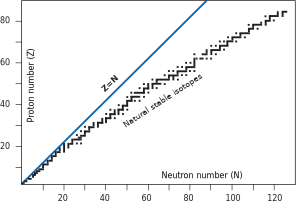
\includegraphics[width=10cm]{../figures/chart-of-nuclides.png}
\captionof{figure}{A schematic `\emph{Chart of Nuclides}' \citep[modified
    from][]{allegre2008}.}
\fi

\section{The age equation}

A characteristic property of radioactive decay is its absolute
independence of external physical and chemical effects. In other
words, it is not affected by changes in pressure, temperature, or the
molecular bonds connecting a radioactive nuclide to neighbouring
atoms. This means that the rate at which a radioactive parent decays
to a radiogenic daughter per unit time, i.e. $dP/dt$ only depends on
$P$, the number of parent atoms present. The \emph{decay constant}
$\lambda$ expresses the likelihood that a radioactive disintegration
takes place in any given time (i.e., $\lambda$ has units of atoms per
atoms per year). This can be expressed mathematically with the
following differential equation:

\begin{equation}
\frac{dP}{dt} = -\lambda P
\label{eq:dPdt}
\end{equation}

Integrating this equation over time yields:

\begin{equation}
P = P_\circ e^{-\lambda t}
\label{eq:P}
\end{equation}

where $P_\circ$ is the number of parent atoms present at time
$t=0$.  Since this number is generally unknown (one exception is
$^{14}$C, see Section \ref{sec:14C}), Equation \ref{eq:P} generally
cannot be used in this form. We can, however, measure the
\emph{present} number of parent and daughter nuclides in the
sample. Rewriting Equation \ref{eq:P}:

\begin{equation}
P_\circ = P e^{\lambda t}
\label{eq:P0}
\end{equation}

and bearing in mind that $P_\circ = P + D$, we obtain:

\begin{equation}
D = P (e^{\lambda t}- 1)
\label{eq:D}
\end{equation}

This equation forms the foundation of most geochronological
methods. It can be rewritten explicitly as a function of time:

\begin{equation}
t = \frac{1}{\lambda} \ln\left(\frac{D}{P} + 1\right)
\label{eq:t}
\end{equation}

The degree of instability of a radioactive nuclide can be expressed by
$\lambda$ or by the \emph{half life} $t_{1/2}$, which is the time
required for half of the parent nuclides to decay. This follows
directly from Equation \ref{eq:P}:

\begin{equation}
\frac{P_\circ}{2} = P_\circ e^{-\lambda t_{1/2}} 
\Rightarrow t_{1/2} = \frac{\ln(2)}{\lambda}
\label{eq:T12}
\end{equation}

As a rule of thumb, the detection limit of a radiometric
geo\-chro\-no\-me\-ter is reached after about 10 half lives. Thus,
$^{14}$C goes back $\sim$50,000 years, $^{10}$Be 10 million and
$^{40}$K 10 billion years.

\section{Decay series}
\label{sec:decay-series}

Sometimes the radiogenic daughter ($D_1$) of a radioactive parent is
radioactive as well, decaying to a daughter of its own ($D_2$), which
may be radioactive again etc., until a stable daughter ($D_*$) is
reached. Considering the simplest case of one intermediate daughter:

\begin{equation}
P \xrightarrow[]{\lambda_P} D_1 \xrightarrow[]{\lambda_1} D_*
\label{eq:series}
\end{equation}

The increase (or decrease) of the number of atoms per unit time for
each of the nuclides is given by:

\begin{align}
\mbox{for~} P &: dP/dt = -\lambda_P P \label{eq:P1}\\
\mbox{for~} D_1 &: dD_1/dt = \lambda_P P - \lambda_1 D_1 \label{eq:D1}\\
\mbox{for~} D_* &: dD_*/dt = \lambda_1 D_1 \label{eq:D*}
\end{align}

The number of parent atoms $P$ can be written as a function of $t$:

\begin{equation}
P = P_\circ e^{-\lambda_P t}
\label{eq:P2}
\end{equation}

Plugging Equation \ref{eq:P2} into \ref{eq:D1} yields

\begin{equation}
dD_1/dt = \lambda_P P_\circ e^{-\lambda_P t} - \lambda_1 D_1
\label{eq:dD1dt}
\end{equation}

Solving this differential equation yields the evolution of $D_1$ with
time. Assuming that $D_1=0$ at $t=0$:

\begin{equation}
D_1 = \frac{\lambda_P}{\lambda_1 - \lambda_P} P_\circ \left[
  e^{-\lambda_P t} - e^{-\lambda_1 t}\right]
\label{eq:ND1}
\end{equation}

If $\lambda_P \ll \lambda_1$ (by a factor of 10 or greater), and $t
\gg 1/\lambda_1$ then $e^{-\lambda_1 t}$ becomes vanishingly small
relative to $e^{-\lambda_P t}$ so that Equation \ref{eq:ND1} can be
simplified:

\begin{equation}
D_1 = \frac{\lambda_P}{\lambda_1 - \lambda_P} P_\circ e^{-\lambda_P t}
\label{eq:ND1b}
\end{equation}

\noindent or, alternatively:

\begin{equation}
D_1 = \frac{\lambda_P}{\lambda_1 - \lambda_P} P
\label{eq:ND1c}
\end{equation}

This means that the ratio of $D_1$ and $P$ remains constant
through time. If $\lambda_P \ll \lambda_1$, then $\lambda_1 -
\lambda_P \approx \lambda_1$, from which it follows that:

\begin{equation}
D_1 = \frac{\lambda_P}{\lambda_1} P
\label{eq:ND1d}
\end{equation}

Rearranging:

\begin{equation}
D_1 \lambda_1 = P \lambda_P
\label{eq:ND1L1}
\end{equation}

or, equivalently:

\begin{equation}
\frac{P}{D_1} = \frac{t_{1/2}(P)}{t_{1/2}(D_1)}
\label{eq:NPND1}
\end{equation}

This is the \emph{secular equilibrium} in which the number of atoms of
both radioactive members is proportional to their respective half
lives. In the geochronological isotope systems $^{235}$U/$^{207}$Pb,
$^{238}$U/$^{206}$Pb and $^{232}$Th/$^{207}$Pb, the lead isotopes are
the end points of a long decay series comprised of several $\alpha$
and $\beta^-$ disintegrations, in which the decay constants of the
parent nuclide is orders of magnitude shorter than the other nuclides
in the chain. For a decay series like that, Equation \ref{eq:ND1L1}
can be generalised to:

\begin{equation}
D_n \lambda_n = \cdots  = D_2 \lambda_2 = D_1 \lambda_1 = P \lambda_P
\label{eq:NDnLn}
\end{equation}

This means that the entire series is in equilibrium, so that all
members occur in mutually constant proportions. The number of atoms of
the stable end member $D_*$ is given by:

\begin{equation}
D_* = P_\circ - P - D_1 - D_2 - \cdots - D_n
\label{eq:ND*}
\end{equation}

Using Equation \ref{eq:NDnLn}, this becomes:

\begin{equation}
D_* = P_\circ - P - \frac{P \lambda_P}{\lambda_1} - 
\frac{P \lambda_P}{\lambda_2} - \cdots - \frac{P \lambda_P}{\lambda_n}
\label{eq:ND*2}
\end{equation}

or

\begin{equation}
D_* = P_\circ - P \left( 1 + \frac{\lambda_P}{\lambda_1} - 
\frac{\lambda_P}{\lambda_2} - \cdots - \frac{\lambda_P}{\lambda_n}\right)
\label{eq:ND*3}
\end{equation}

Since each of the ratios $\lambda_P/\lambda_1$, $\lambda_P/\lambda_2$,
etc.  are vanishingly small, we can simplify Equation \ref{eq:ND*3}
as:

\begin{equation}
D_* = P_\circ - P = P \left( e^{\lambda_P t} -1 \right)
\label{eq:ND*4}
\end{equation}

This means that the accumulation of the final Pb isotope of the
aforementioned three decay series is only a function of the decay of
the parent isotope.  All intermediate decay steps are therefore
inconsequential. In rare cases, however, the isotopic equilibrium is
disturbed by a dissolution or recrystallisation event, say. The
intermediate parent/daughter pairs can then be used to date phenomena
occurring over much shorter time scales than those probed by the U-Pb
method (Section \ref{ch:intro2Useries}).

\begin{figure}[!ht]
  \captionsetup{width=11cm}
  \centering
  \ifpdf
  \ifuclnotes
  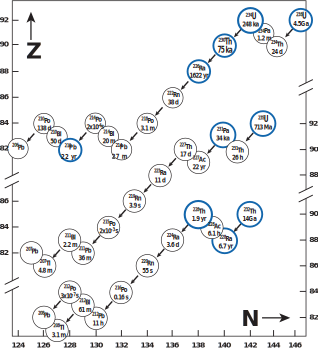
\includegraphics[width=\textwidth]{../figures/U-Th-series.pdf}
  \else
  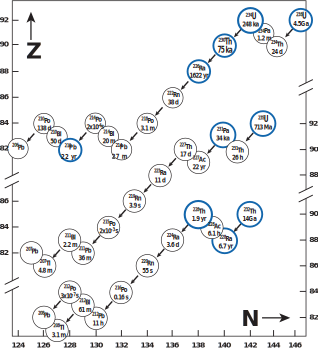
\includegraphics[width=12cm]{../figures/U-Th-series.pdf}
  \fi
  \else
  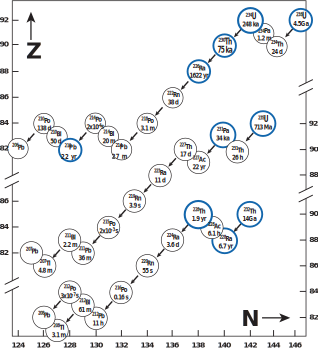
\includegraphics[width=11cm]{../figures/U-Th-series.png}
  \fi
  \caption{The decay series of $^{232}$Th, $^{235}$U and $^{238}$U,
    which form the basis of the U-Th-Pb, U-Th-He and U-Th-series methods
    \citep[modified from][]{allegre2008}.}
  \label{fig:U-Th-series}
\end{figure}


\chapter{Analytical techniques}
\label{ch:analyticaltechniques}

Isotope geochemistry is based on the accurate and precise
determination of elemental and isotopic compositions of rocks and
minerals.  Although some of the earliest geochronological methods
(notably the $^{14}$C method, see Section \ref{sec:14C}) were based on
the detection of radioactivity by means of Geiger-M\"{u}ller counters
and liquid scintillation detectors, nearly all modern isotope
geochemistry is done by mass spectrometry.

\section{Mass spectrometry}
\label{sec:mass-specs}

A mass spectrometer is a device that separates electrically charged
atoms or molecules based on their mass, enabling precise measurement
of the isotopic composition. A mass spectrometer consists of the
following parts:

\begin{enumerate}
\item ion source: this can be either a filament (similar to that found
  in an incandescent light bulb), a plasma torch, a primary ion beam,
  or a spray chamber, among other possibilities.
\item mass analyser: this can be an electromagnet (possibly combined
  with an electrostatic field), or a rapidly fluctuating electric
  field.
\item ion detector: this is, essentially, a volt meter.
\end{enumerate}

In the remainder of this section, we will assume the source to be a
filament and the mass analyser to be an electromagnet. \\

After pumping the mass spectrometer down to (ultra-)high vacuum
conditions (10$^{-6}$ to 10$^{-9}$ mbar), the sample enters the ion
source as a gas, where it is bombarded with electrons.  The resulting
ions (with charge $e$) are accelerated in an electric field (with
potential difference $V$) and collimated to a narrow beam. This beam
is sent through a magnetic field (with strength $H$) which deflects it
into a circular trajectory with a radius proportional to the ion mass
($m$).  This results in a physical separation of the incoming ion beam
into various outgoing beams. The beams of interest are steered into
the ion detector which, in its simplest design (the so-called `Faraday
Cup') consists of a long and narrow cup. The ion beam is neutralised
in the cup by electrons flowing from ground through a resistor. The
potential difference across this resistor is measured and registered
on a computer for further processing.\\

The electric field transfers a certain amount of kinetic energy to the
ions:

\begin{equation}
E = e V = \frac{m v^2}{2}
\label{eq:E}
\end{equation}

With $e$ is the electrical charge (in multiples of 1.60219 $\times
10^{-19}$C, which is the elementary charge of an electron.  Because
each type of ion has a different mass ($m$, in multiples of 1.660538
$\times 10^{-27}$kg, the atomic mass unit), their terminal velocity
($v$) differs as well:

\begin{equation}
v = \sqrt{\frac{2 e V}{m}}
\label{eq:v}
\end{equation}

The mass analyser deflects the ions according to the following equation:

\begin{equation}
H e v = \frac{m v^2}{r}
\label{eq:Hev}
\end{equation}

Substituting Equation \ref{eq:v} into \ref{eq:Hev} yields:

\begin{equation}
H \sqrt{\frac{2 e V}{m}} = \frac{2 V}{r}
\label{eq:H2eVm}
\end{equation}

from which it follows that:

\begin{equation}
\begin{array}{rl}
~ & r = \frac{1}{H}\sqrt{\frac{2 m V}{e}} \\
and~ & H = \frac{1}{r}\sqrt{\frac{2 m V}{e}}\\
\end{array}
\label{eq:rH}
\end{equation}

Equation \ref{eq:rH} allows us to calculate the radius of the ion
trajectory for any given mass-to-charge ratio $m/e$. Note that light
isotopes are more strongly deflected than equally charged heavy ones.
Equation \ref{eq:rH} can also be used to calculate the magnetic field
strength required to deflect an ion beam with a given $m/e$ ratio into
the collector.  This is more practical because most mass spectrometers
have a fixed radius so that the different ions must be collected by
varying $H$. Some modern mass spectrometers are equipped with multiple
ion collectors the enabling simultaneous analysis of several ionic
masses.

\begin{figure}[!ht]
  \centering
  \ifpdf
  \def\svgwidth{\textwidth}
  \input{mass-spec.pdf_tex}
  \else
  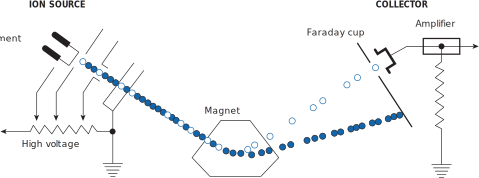
\includegraphics[width=10cm]{../figures/mass-spec.png}
  \fi
  \caption{Schematic diagram of a sector-field noble gas or TIMS mass
    spectrometer \citep[modified from][]{allegre2008}.}
  \label{fig:mass-spec}
\end{figure}

Several types of mass spectrometers are used for geoscience
applications:

\begin{enumerate}
\item{\emph{Thermal Ionisation Mass Spectrometry (TIMS)}.}\\ The
  sample is dissolved and subjected to careful chemical separation
  procedures (liquid chromatography) in order to separate the parent
  and daughter elements to a high level of purity. The resulting
  solutions are spiked and deposited on a tungsten or tantalum
  filament, which is brought to a glow by an electric current and thus
  produces ions. These are separated by a large electromagnet and
  analysed in one or more Faraday cups. TIMS is very time consuming
  but produces extremely precise results (\permil-level precision on
  the ages).
 
\item{\emph{Inductively Coupled Plasma Mass Spectrometry
    (ICP-MS)}.}\\ The sample is vapourised in one of two ways: either
  by introducing a liquid into a spray chamber, or by firing an
  ultraviolet laser at a solid sample and transporting the resulting
  aerosol into the ion source with a carrier gas (typically
  helium). The ion source itself consists of an argon flow which is
  heated to a temperature of approximately 10,000K by sending a
  radiofrequency current through a coil. This breaks up all the
  molecular bonds and produces a plasma (i.e. a `soup' of ions and
  electrons) which enters the high vacuum chamber through a tiny
  opening.  The mass analyser can either be a sector magnet or a
  quadrupole (which consists of four metal rods generating a rapidly
  fluctuating electrical field). ICP-MS offers a higher throughput
  than TIMS, especially in laser ablation mode, where hundreds of ages
  can be measured per day. However, this increased throughput comes at
  the expense of precision, which is on the percent level (better in
  solution mode).

\item{\emph{Secondary ion mass spectrometry (SIMS)}}\\ Prior to the
  development of laser ablation (LA-) ICP-MS, the only other method to
  produce spot measurements in solid samples was by firing a beam of
  negative (e.g. oxygen) or positive (e.g. caesium) ions at the target
  under high vacuum.  This releases (`sputters') positive (or
  negative, in the case of a Cs beam) \emph{secondary} ions from the
  sample surface, which are accelerated by an electrostatic field and
  sent to a sector field mass spectrometer. Although SIMS has been
  replaced by LA-ICP-MS in some applications, it remains an important
  instrument in the geochronological toolbox because (a) it offers
  higher spatial resolution than laser ablation (5-10$\mu m$
  vs. 25-50$\mu m$) and (b) can measure light ions (e.g, hydrogen)
  more reliably than LA-ICP-MS.

\item{\emph{Noble gas mass spectrometry}}\\ The noble gases (He, Ne,
  Ar, Kr, Xe) require a different class of mass spectrometer than the
  rest of the periodic table because, as their name suggests: 1) they
  are gases 2) that do not ionise easily. Noble gasses are liberated
  from solid state materials by heating or laser ablation under
  ultra-high vacuum conditions. To remove any unwanted gas species
  (such as CO, CO\textsubscript{2}, hydrocarbons, etc.) that may
  interfere with the noble gas measurements, the released gas is
  exposed to reactive metals, liquid N\textsubscript{2} `cold traps'
  and other `gettering' devices in a `noble gas extraction line' for a
  duration of 5--30 minutes. The extraction line removes all the
  reactive gas species until only the inert noble gases remain. It is
  only after this lengthy delay that the purified noble gases are
  ionised by electron bombardment, and analysed on the actual mass
  spectrometer.
  
\item{\emph{Accelerator Mass Spectrometer (AMS)}}\\ The AMS combines
  two mass spectrometers with a (`tandem' type) particle accelerator.
  Ions are produced by a SIMS source and steered through a first mass
  analyser, which selects all ions of a desired mass (e.g., mass 14:
  $^{14}$C$^-$, ${}^{12}$CH$_2^-$, $\cdots$). The resulting beam is
  accelerated in the first part of the tandem accelerator by a
  potential difference of several million eV, and sent through a thin
  chamber filled with a `stripper' gas. Collisions of stripper gas
  atoms with the incoming ions destroys any molecular bonds and forms
  3+ ions in the process. The beam now consists of purely atomic ions,
  which are accelerated in the second part of the accelerator and
  steered into a second mass analyser. The AMS has revolutionised the
  $^{14}$C method by enabling the analysis of extremely small
  (mg-sized) samples (see Section \ref{sec:14C}), and has enabled a
  whole new field of geochronology based on the analysis of
  terrestrial cosmogenic radionuclides\ifuclnotes (Chapter
  \ref{sec:cosmo})\fi. The main limitation of AMS is its high
  cost. Currently only two AMS facilities are operating in the UK (in
  Oxford and Glasgow).
\end{enumerate}

\begin{figure}[!ht]
  \centering
  \ifpdf
  \def\svgwidth{\textwidth}
  \input{AMS.pdf_tex}
  \else
  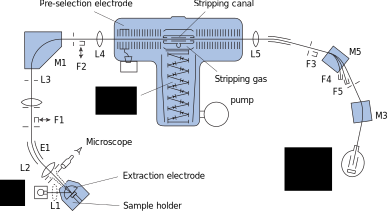
\includegraphics[width=10cm]{../figures/AMS.png}
  \fi
  \caption{Schematic diagram of an Accelerator Mass Spectrometer (AMS)
    \citep[modified from][]{allegre2008}.}
  \label{fig:AMS}
\end{figure}

\section{Isotope dilution}
\label{sec:isotope-dilution}

Besides determining isotopic compositions, the mass spectrometer can
also be used to measure elemental concentrations, using a method
called \emph{isotope dilution}. This is done by mixing the sample
solution (whose isotopic composition has already been determined) with
a known quantity of a solution with a different (but known) isotopic
composition and known elemental concentration. The latter solution is
called the \emph{spike}.  The isotopic composition of the mixture is
analysed by mass spectrometry.  The measured isotopic ratio $R_m$ for
an element with two isotopes ($^aX$ and $^{b}X$) is given by:

\begin{equation}
R_m = \frac{N {}^aX_N + S {}^aX_S}{N {}^bX_N + S {}^bX_S}
\label{eq:Rm}
\end{equation}

with

\begin{equation*}
\begin{array}{rl}
N = & \mbox{the number of atoms of X in the sample}\\
S = & \mbox{the number of atoms of X in the spike}\\
^aX_N, {}^bX_N = & \mbox{the atomic abundance of isotope~} a \mbox{~(or b) in the~}\\
{}^aX_S, {}^bX_S ~~~ & \mbox{sample (or spike)} (^aX_N + {}^bX_N = {}^aX_S + {}^bX_S = 1)
\end{array}
\end{equation*}

$N$ is the only unknown in Equation \ref{eq:Rm}, which can therefore be
rewritten as:

\begin{equation}
N = S \frac{^aX_S - R_m {}^bX_S}{R_m {}^bX_N - {}^aX_N}
\label{eq:N}
\end{equation}

$N$ can also be expressed as a function of the isotopic ratios in the
sample $R_N (={}^aX_N/{}^bX_N)$ and in the spike $R_S
(={}^aX_S/{}^bX_S)$. The atomic abundance of $^aX$ and $^bX$ in the
sample are given by:

\begin{equation}
^aX_N = \frac{R_N}{R_N + 1} \mbox{~and~} {}^bX_N = \frac{1}{R_N + 1}
\label{eq:aXNbXN}
\end{equation}

and in the spike:

\begin{equation}
^aX_S = \frac{R_S}{R_S + 1} \mbox{~and~} {}^bX_S = \frac{1}{R_S + 1}
\label{eq:aXSbXS}
\end{equation}

Substituting Equations \ref{eq:aXSbXS} and \ref{eq:aXNbXN} into
\ref{eq:N} yields:

\begin{equation}
N = S \frac{(R_N+1)(R_S-R_m)}{(R_S+1)(R_m-R_N)}
\label{eq:N2}
\end{equation}

Equations \ref{eq:N} and \ref{eq:N2} give the atomic concentration of
$X$ (in atoms/g).  Dividing $N$ by Avogadro's number $N_A$ and
multiplying with the atomic weights (g/mol) yields the corresponding
weight percentages. Isotope dilution is a very powerful method
because:

\begin{enumerate}
\item It does not require quantative separation of the elements of
  interest.
\item Chemical purification removes unwanted interferences from other
  species.
\item The method is very sensitive, so extremely low concentrations
  can be measured (ppb or less).
\end{enumerate}

\section{Sample-standard bracketing}
\label{sec:bracketing}

Isotope dilution is the `gold standard' for isotope geochemistry,
recommended when the most accurate and precise results are
desired. Unfortunately, isotope dilution is also very time consuming
and cannot be readily applied to micro-analytical techniques such as
LA-ICP-MS and SIMS. In those cases, and alternative method is used,
which is less precise (\%- rather than \permil- level precision) but
quicker.  The idea is to normalise the signal ratios recorded by the
mass spectrometer to a standard of known age.  As before, let P be a
radioactive parent which decays to a radiogenic daughter D. Suppose
that we can measure both nuclides on the same mass spectrometer,
yielding two electronic signal intensities $S_P$ and $S_D$. These
signals may be recorded in units of V, A, or Hz. We cannot directly
use the signal ratios as a proxy for the isotopic ratio:

$$\frac{D}{P} \neq \frac{S_D}{S_P}$$

because the parent and daughter are two different elements with
different chemical properties and ionisation efficiencies. We can,
however, assume that the isotopic ratio is proportional to the signal
ratio:

\begin{equation}
\frac{D}{P} = C \frac{S_D}{S_P}
\label{eq:eqC}
\end{equation}

Thus, if we double $D$ (and thus $D/P$), we would also expect to
double $S_D$ (and thus $S_D/S_P$). To determine the constant of
proportionality $C$, we analyse a standard of known age ($t_s$) and,
hence ($D/P$)-ratio (due to Equation \ref{eq:D}):

\begin{equation}
C = \left(e^{\lambda_Pt_s} - 1\right) \frac{S^s_P}{S^s_D}
\label{eq:const}
\end{equation}

where $\lambda_P$ is the decay constant of the parent and
$S^s_P/S^s_D$ is the (inverse) signal ratio of the standard.


\chapter{Simple parent-daughter pairs}
\label{ch:intro2PD}

\section{$^{14}$C dating}
\label{sec:14C}

There are two stable isotopes of carbon: $^{12}$C and $^{13}$C, and
one naturally occurring radionuclide: $^{14}$C. The half life of
$^{14}$C is only 5,730 years, which is orders of magnitude shorter
than the age of the Earth. Therefore, no primordial radiocarbon
remains and all $^{14}$C is \emph{cosmogenic}\ifuclnotes (see Section
\ref{sec:cosmo} for related methods)\fi.  The main production
mechanism is through secondary cosmic ray neutron reactions with
$^{14}$N in the stratosphere: $^{14}_7$N (n,p) $^{14}_6$C. Any newly
formed $^{14}$C rapidly mixes with the rest of the atmosphere creating
a spatially uniform carbon composition, which is incorporated into
plants and the animals that eat them. Prior to the industrial
revolution, a gram of fresh organic carbon underwent 13.56 ($\beta^-$)
decays per minute. When a plant dies, it ceases to exchange carbon
with the atmosphere and the $^{14}$C concentration decays with time
according to Equation \ref{eq:dPdt}:

\begin{equation}
\frac{d^{14}C}{dt} = -\lambda_{14} \times {}^{14}C
\label{eq:d14Cdt}
\end{equation}

where $\lambda_{14}$ = 0.120968 kyr$^{-1}$. Thus, the radiocarbon
concentration is directly proportional to the radioactivity, which can
be measured by $\beta$-counting. This can then be used to calculate
the radiocarbon age by rearranging Equation \ref{eq:P}:

\begin{equation}
t = -\frac{1}{\lambda_{14}}
\ln\left[\frac{d{}^{14}C/dt}{(d{}^{14}C/dt)_\circ}\right]
\label{eq:t14C}
\end{equation}

where $(d^{14}C/dt)_\circ$ is the original level of $\beta$ activity.
This method was developed by Willard Libby in 1949, for which he was
awarded the Nobel Prize in 1960. As mentioned before,
$(d^{14}C/dt)_\circ$ was 13.56 prior to the industrial revolution,
when thousands of tonnes of `old' carbon were injected into the
atmosphere, resulting in a gradual lowering of the radiocarbon
concentration until 1950, when nuclear testing produced an opposite
effect, leading to a doubling of the atmospheric $^{14}$C activity in
1963. Since the banning of atmospheric nuclear testing, radiocarbon
concentrations have steadily dropped until today, where they have
almost fallen back to their pre-industrial levels. But even prior to
these anthropogenic effects, $^{14}$C concentrations underwent
relatively large fluctuations as a result of secular variations of the
Earth's magnetic field and, to a lesser extent, Solar activity. These
variations in $(d^{14}C/dt)_\circ$ can be corrected by comparison with
a precisely calibrated production rate curve, which was constructed by
measuring the $^{14}$C activity of tree rings
(\emph{dendrochronology}).\\

Since the 1980's, $\beta$-counting has been largely replaced by
accelerator mass spectrometry (AMS, see Section \ref{sec:mass-specs}),
in which the $^{14}$C concentration is measured directly relative to a
stable isotope such as $^{13}$C. Although this has not significantly
pushed back the age range of the radiocarbon method, it has
nevertheless revolutionised the technique by reducing the sample size
requirements by orders of magnitude. It is now possible to analyse
individual seeds or tiny fragments of precious objects such as the
Turin Shroud, which was dated at AD1260-1390.

\section{The Rb-Sr method}
\label{sec:Rb-Sr}

Trace amounts of Rb and Sr are found in most minerals as substitutions
for major elements with similar chemical properties. Rb is an alkali
metal that forms single valent positive ions with an ionic radius of
1.48 \AA, which is similar to K$^+$ (1.33 \AA).  Rb is therefore
frequently found in K-bearing minerals such as micas, K-feldspar and
certain clay minerals. Strongly evolved alkalic rocks such as
syenites, trachites and rhyolites often contain high Rb
concentrations.  Rb contains two isotopes of constant abundance:
$^{85}$Rb (72.1854\%) and $^{87}$Rb (27.8346\%). Sr is an alkaline
earth metal that forms bivalent positive ions with a radius of 1.13
\AA, similar to Ca$^{2+}$ (ionic radius 0.99 \AA). It therefore
substitutes Ca$^{2+}$ in many minerals such as plagioclase, apatite,
gypsum and calcite in sites with 8 neighbours, but not in pyroxene
where Ca$^{2+}$ has a coordination number of 6. Native Sr$^{2+}$ can
also substitute K$^+$ in feldspars (where radiogenic Sr is expected to
be found), but this substitution is limited and requires the
simultaneous replacement of Si$^{4+}$ by Al$^{3+}$ in order to
preserve electric neutrality.  Sr therefore predominantly occurs in
Ca-rich undifferentiated rocks such as basalts. Sr contains four
isotopes ($^{84}$Sr, $^{86}$Sr, $^{87}$Sr and $^{88}$Sr) with variable
abundance due to the variable amount of radiogenic $^{87}$Sr. However,
the non-radiogenic $^{84}$Sr/$^{86}$Sr and $^{86}$Sr/$^{88}$Sr-ratios
are constant with values of 0.056584 and 0.1194, respectively. The
Rb-Sr chronometer is based on the radioactive decay of $^{87}$Rb to
$^{87}$Sr:

\begin{equation}
{}^{87}Rb \rightarrow {}^{87}Sr + \beta^- + \nu +
0.275 MeV
\label{eq:87Rb}
\end{equation}

Where $\nu$ indicates an antineutrino. The number of radiogenic
${}^{87}$Sr atoms produced by this reaction after a time t is given
by:

\begin{equation}
{}^{87}Sr^* = {}^{87}Rb (e^{\lambda_{87} t} - 1)
\label{eq:87Sr*}
\end{equation}

where $^{87}Rb$ is the actual number of $^{87}$Rb atoms per unit
weight and $\lambda_{87}$ is the decay constant 1.42 $\times$
10$^{-11}$ yr$^{-1}$ (t$_{1/2}$ = 4.88$\times$10$^{10}$yr).  In
addition to this radiogenic $^{87}$Sr, most samples will also contain
some `ordinary' Sr. The total number of $^{87}$Sr atoms measured is
therefore given by:

\begin{equation}
^{87}Sr = {}^{87}Sr^* + {}^{87}Sr_\circ
\label{eq:87Sr}
\end{equation}

with $^{87}Sr_\circ$ the initial $^{87}$Sr present at the time of
isotopic closure.  Combining Equations \ref{eq:87Sr} and
\ref{eq:87Rb}, we obtain:

\begin{equation}
^{87}Sr = {}^{87}Sr_\circ + {}^{87}Rb (e^{\lambda_{87} t} - 1)
\label{eq:87Sr2}
\end{equation}

Dividing this by the non-radiogenic $^{86}$Sr yields

\begin{equation}
\frac{^{87}Sr}{^{86}Sr} =
\left(\frac{^{87}Sr}{^{86}Sr}\right)_\circ +
\frac{^{87}Rb}{^{86}Sr} (e^{\lambda_{87} t} - 1)
\label{eq:87Sr86Sr}
\end{equation}

The method can be applied to single minerals or to whole rocks.  Given
the very long half life, the optimal time scale ranges from the
formation of the solar system to the late Palaeozoic (300-400 Ma).  To
measure a Rb/Sr age, the weight percentage of Rb is measured by means
of X-ray fluorescence, ICP-OES or similar techniques, and the
$^{87}$Sr/$^{86}$Sr ratio is determined by mass spectrometry (isotope
dilution). The $^{87}$Rb/$^{86}$Sr-ratio is then calculated as:

\begin{equation}
\frac{^{87}Rb}{^{86}Sr} =
\frac{Rb}{Sr} \frac{Ab(^{87}Rb)
  M(Sr)}{Ab(^{86}Sr) M(Rb)}
\label{eq:87Rb86Sr}
\end{equation}

Where $Ab(\cdot)$ signifies `abundance' and $M(\cdot)$ `molar mass'.

\section{Isochrons}
\label{sec:isochrons}

Equation \ref{eq:87Rb86Sr} can be used in one of two ways. A first
method is to use an assumed value for $(^{87}$Sr$/^{86}$Sr)$_\circ$,
based on the geological context of the sample. This method is only
reliable for samples with a high Rb/Sr ratio (e.g., biotite) because
in that case, a wrong value for $({}^{87}$Sr$/{}^{86}$Sr$)_\circ$ has
only a minor effect on the age. A second and much better method is to
analyse several minerals of the same sample and plot them on a
$(^{87}$Rb$/^{86}$Sr) vs.  (${}^{87}$Sr$/{}^{86}$Sr) diagram (Figure
\ref{fig:isochron}).  Due to Equation \ref{eq:87Sr86Sr}, this should
form a linear array (the so-called \emph{isochron}) with slope
$(e^{\lambda_{87} t} - 1)$ and intercept
$({}^{87}Sr/{}^{86}Sr)_\circ$.  Both parameters can be determined
by linear regression, allowing us to quantify the `goodness of fit' of
the data and obviating the need to assume any initial Sr-ratios.

\ifpdf
\ifuclnotes
\begin{figure}[!ht]
  \centering
  \def\svgwidth{.7\textwidth}
  \input{isochron.pdf_tex}
  \caption{Schematic evolution of the $^{87}$Sr$/{}^{86}$Sr-system as
    a function of time for multiple aliquots of a hypothetical sample
    with initial ratio $({}^{87}$Sr$/{}^{86}$Sr$)_\circ$=0.700. The
    slope of the isochron is a function of the age as per Equation
    \ref{eq:87Sr86Sr} \citep[modified from][]{allegre2008}.}
  \label{fig:isochron}
\end{figure}
\else % end of uclnotes
\begin{figure}[!ht]
\noindent\begin{minipage}[t]{.6\textwidth}
\strut\vspace*{-\baselineskip}\newline
\def\svgwidth{\textwidth}
\input{isochron.pdf_tex}
\end{minipage}
\begin{minipage}[t]{.4\textwidth}
  \captionof{figure}{Schematic evolution of the $^{87}$Sr$/{}^{86}$Sr-system as
    a function of time for multiple aliquots of a hypothetical sample
    with initial ratio $({}^{87}$Sr$/{}^{86}$Sr$)_\circ$=0.700. The
    slope of the isochron is a function of the age as per Equation
    \ref{eq:87Sr86Sr} \citep[modified from][]{allegre2008}.}
  \label{fig:isochron}
\end{minipage}
\end{figure}
\fi % end of pdf
\else
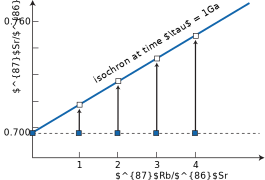
\includegraphics[width=10cm]{../figures/isochron.png}
  \captionof{figure}{Schematic evolution of the $^{87}$Sr$/{}^{86}$Sr-system as
    a function of time for multiple aliquots of a hypothetical sample
    with initial ratio $({}^{87}$Sr$/{}^{86}$Sr$)_\circ$=0.700. The
    slope of the isochron is a function of the age as per Equation
    \ref{eq:87Sr86Sr} \citep[modified from][]{allegre2008}.}
  \label{fig:isochron}
\fi

\section{The Sm-Nd method}
\label{sec:Sm-Nd}

The elements Neodymium (Z=60) and Samarium (Z=62) are so-called `rare
earth elements'.  All elements of this family have similar chemical
properties. They nearly all form 3+ ions of roughly equal albeit
slightly decreasing size with atomic number.  The ionic radius of Nd
and Sm is 1.08 and 1.04 \AA, respectively.  As the name suggests, rare
earth elements rarely form the major constituents of minerals.  One
notable exception is monazite, which is a rare earth phosphate. In
most cases, the rare earth elements are found in trace amounts of up
to 0.1\% in apatite [Ca$_5$(PO$_4$)$_3$(OH,Cl,F)] and zircon
[ZrSiO$_4$]. Both Sm and Nd are slightly enriched in feldspar, biotite
and apatite and thus tend to be found in higher concentrations in
differentiated (alkalic) magmatic rocks.\\

Because their chemical properties are so similar, geological processes
are rarely capable of fractionating the Sm and Nd
concentrations. Therefore, the Sm/Nd ratio in most rocks generally
falls in a narrow range of 0.1 to 0.5 (the Sm/Nd ratio of the solar
system being 0.31). One exception is garnet, in which Sm/Nd ratios $>$
1 have been found. Partial melting of mafic minerals such as pyroxene
and olivine produces lower Sm/Nd ratios in the fluid phase than the
solid residue.  The Sm/Nd ratio of magmatic rocks therefore decreases
with increasing differentiation.\\

Natural Sm contains seven naturally occurring isotopes, three of which
are radioactive ($^{147}$Sm, $^{148}$Sm and $^{149}$Sm). Only
$^{147}$Sm has a sufficiently short half life to be useful for
geochronology.  Nd also contains seven isotopes, of which only one is
radioactive ($^{144}$Nd) but with a very long half life. $^{143}$Nd is
the radiogenic daughter of $^{147}$Sm and is formed by
$\alpha$-decay. This forms the basis of the Sm-Nd chronometer.
Analogous to the Rb-Sr method (Equation \ref{eq:87Sr*}), we can write:

\begin{equation}
^{143}Nd^* = {}^{147}Sm (e^{\lambda_{147} t} - 1)
\label{eq:144Nd*}
\end{equation}

Hence:

\begin{equation}
t = \frac{1}{\lambda_{147}}
\ln\left(\frac{^{143}Nd^*}{^{147}Sm} + 1 \right)
\label{eq:tNd}
\end{equation}

With $\lambda_{147}$ = 6.54$\times$10$^{-12} $yr$^{-1}$ ($t_{1/2}$ =
1.06$\times$10$^{11}$yr).  Since most samples contain some initial Nd,
the preferred way to calculate Sm/Nd ages is by analysing several
minerals in a rock and create an isochron, similar to the Rb/Sr method
(Section \ref{sec:isochrons}):

\begin{equation}
\frac{^{143}Nd}{^{144}Nd} =
\left(\frac{^{143}Nd}{^{144}Nd}\right)_{\circ} +
\frac{^{147}Sm}{^{144}Nd} \left(e^{\lambda_{147}t} -
1\right)
\label{eq:143Nd147Nd}
\end{equation}

All measurements are done by mass spectrometry using isotope dilution.
Because of the identical atomic masses of $^{147}$Sm and $^{147}$Nd,
it is necessary to perform a chemical separation between Sm and Nd
prior to analysis.\\

The Sm/Nd method is generally applied to basic and ultrabasic igneous
rocks (basalt, peridotite, komatiite) of Precambrian to Palaeozoic
age. The method thus complements the Rb/Sr method, which is
preferentially applied to acidic rock types. The Sm/Nd method can also
be applied to high grade metamorphic rocks (granulites, eclogites) as
well as meteorites (shergottites, nahklites). Since the rare earths
are significantly less mobile than Rb and Sr, the Sm/Nd is more
reliable in rocks that have been disturbed by weathering or
metamorphism.


\chapter{The U-Pb system}
\label{sec:U-Pb}

U and Th are found on the extremely heavy end of the Periodic Table of
Elements.  All their isotopes are radioactive and exhibit
$\alpha$-decay and sometimes even spontaneous fission (see Section
\ref{sec:fission-tracks}). $^{232}$Th, $^{235}$U and $^{238}$U each
form the start of long decay series comprising multiple $\alpha$- and
$\beta$ emissions which eventually produce various isotopes of Pb:

\begin{equation}
\begin{array}{rl}
^{238}U \rightarrow & {}^{206}Pb + 8\alpha + 6\beta + 47\mbox{MeV} \\ 
^{235}U \rightarrow & {}^{207}Pb + 7\alpha + 4\beta + 45\mbox{MeV} \\
^{232}Th \rightarrow & {}^{208}Pb + 6\alpha + 4\beta + 40\mbox{MeV} 
\end{array}
\label{eq:UThdecay}
\end{equation}

Each of these three decay series is unique, i.e. no isotope occurs in
more than one series (Figure \ref{fig:U-Th-series}). Furthermore, the
half life of the parent isotope is much longer than any of the
intermediary daughter isotopes, thus fulfilling the requirements for
secular equilibrium (Section \ref{sec:decay-series}). We can therefore
assume that the $^{206}$Pb is directly formed by the $^{238}$U, the
$^{207}$Pb from the $^{235}$U and the $^{208}$Pb from the
$^{232}$Th. Several chronometers are based on the $\alpha$-decay of U
and Th:

\begin{itemize}
\item The U-Th-Pb method (Section \ref{sec:U-Th-Pb})
\item The Pb-Pb method (Section \ref{sec:Pb-Pb})
\item The U-Th-He method (Section \ref{sec:U-Th-He})
\end{itemize}

\section{The U-(Th-)Pb method}
\label{sec:U-Th-Pb}

Natural Pb consists of four isotopes $^{204}$Pb, $^{206}$Pb,
$^{207}$Pb and $^{208}$Pb. The ingrowth equations for
the three radiogenic Pb isotopes are given by:

\begin{equation}
  \begin{array}{rl}
    &{}^{206}Pb^* = {}^{238}U \left(e^{\lambda_{238}t} - 1\right)\\ 
    &{}^{207}Pb^* = {}^{235}U \left(e^{\lambda_{235}t} - 1\right)\\ 
    &{}^{208}Pb^* = {}^{232}Th \left(e^{\lambda_{232}t} - 1\right)
  \end{array}
  \label{eq:Pb*}
\end{equation}

With $\lambda_{238}$ = 1.55125 $\times 10^{-10} a^{-1}$ (t$_{1/2}$ =
4.468 Gyr), $\lambda_{235}$ = 9.8485 $\times 10^{-10} a^{-1}$
(t$_{1/2}$ = 703.8 Myr), and $\lambda_{232}$ = 0.495 $\times 10^{-10}
a^{-1}$ (t$_{1/2}$ = 14.05 Gyr). The corresponding age equations are:

\begin{equation}
  \begin{array}{rl}
    t_{206} & = \frac{1}{\lambda_{238}}
    \ln \left(\frac{{}^{206}Pb^*}{{}^{238}U}+1\right)\\
    t_{207} & = \frac{1}{\lambda_{235}}
    \ln \left(\frac{{}^{207}Pb^*}{{}^{235}U}+1\right)\\
    t_{208} & = \frac{1}{\lambda_{232}}
    \ln \left(\frac{{}^{208}Pb^*}{{}^{232}Th}+1\right)
  \end{array}
  \label{eq:tPb*}
\end{equation}

Some igneous minerals (notably zircon) conveniently incorporate lots
of U and virtually no Pb upon crystallisation. For those minerals, the
non-radiogenic Pb can be safely neglected (at least for relatively
young ages), so that we can assume that $Pb \approx Pb^*$. This
assumption cannot be made for other minerals, young ages, and high
precision geochronology. In those cases, the inherited component (aka
`common Pb') needs to be quantified, which is done by normalising to
non-radiogenic $^{204}$Pb:

\begin{equation}
\begin{array}{c}
  \frac{^{206}Pb}{^{204}Pb} = \left(\frac{^{206}Pb}{^{204}Pb}\right)_\circ +
  \frac{^{238}U}{^{204}Pb} \left(e^{\lambda_{238}t} - 1\right) \\
  \frac{^{207}Pb}{^{204}Pb} = \left(\frac{^{207}Pb}{^{204}Pb}\right)_\circ +
  \frac{^{235}U}{^{204}Pb} \left(e^{\lambda_{235}t} - 1\right)\\
  \frac{^{208}Pb}{^{204}Pb} = \left(\frac{^{208}Pb}{^{204}Pb}\right)_\circ +
  \frac{^{232}Th}{^{204}Pb} \left(e^{\lambda_{232}t} - 1\right)
\end{array}
\label{eq:Pb}
\end{equation}

where $\left(\frac{^{x}Pb}{^{204}Pb}\right)_\circ$ stands for the
common Pb component for isotope x. The corresponding age equations
then become:

\begin{equation}
\begin{array}{c}
  t_{206}=\frac{1}{\lambda_{238}}\ln\left(\frac{\left(\frac{^{206}Pb}{^{204}Pb}\right)-
    \left(\frac{^{206}Pb}{^{204}Pb}\right)_\circ}{\frac{^{238}U}{^{204}Pb}}+1\right)\\
  t_{207}=\frac{1}{\lambda_{235}}\ln\left(\frac{\left(\frac{^{207}Pb}{^{204}Pb}\right)-
    \left(\frac{^{207}Pb}{^{204}Pb}\right)_\circ}{\frac{^{235}U}{^{204}Pb}}+1\right)\\
  t_{208}=\frac{1}{\lambda_{232}}\ln\left(\frac{\left(\frac{^{208}Pb}{^{204}Pb}\right)-
    \left(\frac{^{208}Pb}{^{204}Pb}\right)_\circ}{\frac{^{232}Th}{^{204}Pb}}+1\right)
\end{array}
\label{eq:tPb}
\end{equation}

U-Pb dating grants access to two separate geochronometers
($^{206}$Pb/${}^{238}$U and $^{207}$Pb/${}^{235}$U) based on different
isotopes of the same parent-daughter pair (i.e. U \& Pb).  This
built-in redundancy provides a powerful internal quality check which
makes the method arguably the most robust and reliable dating
technique in the geological toolbox. The initial Pb composition can
either be determined by analysing the Pb composition of a U-poor
mineral (e.g., galena or feldspar) or by applying the isochron method
to samples with different U and Th concentrations. As is the case for
any isotopic system, the system needs to remain `closed' in order to
yield meaningful isotopic ages.  This sometimes is not the case,
resulting in a loss of Pb and/or U.  Such losses cause the
$^{206}$Pb/$^{238}$U- and $^{207}$Pb/$^{235}$U-clocks to yield
different ages. Note that isotopic closure is required for all
intermediary isotopes as well.  Critical isotopes are the highly
volatile $^{226}$Rn (t$_{1/2}$=1.6ka) and $^{222}$Rn
(t$_{1/2}$=3.8d). Initially, the U-Pb method was applied to U-ores,
but nowadays it is predominantly applied to accessory minerals such
zircon and, to a lesser extent, apatite, monazite and allanite.

\section{The Pb-Pb method}
\label{sec:Pb-Pb}

The $^{207}$Pb/$^{206}$Pb method is based on the U-Pb method and is
obtained by dividing the two U-Pb members of Equation \ref{eq:Pb*} (or
\ref{eq:Pb}), and taking into account that the average natural
$^{238}$U/$^{235}$U-ratio is 137.818:

\begin{equation}
\frac{^{207}Pb^*}{^{206}Pb^*} = 
\frac{\left(\frac{^{207}Pb}{^{204}Pb}\right)-\left(\frac{^{207}Pb}{^{204}Pb}\right)_\circ}
{\left(\frac{^{206}Pb}{^{204}Pb}\right)-\left(\frac{^{206}Pb}{^{204}Pb}\right)_\circ}
= \frac{1}{137.818} \frac{e^{\lambda_{235}t}-1}{e^{\lambda_{238}t}-1}
\label{eq:PbPb}
\end{equation}

The left hand side of this equation contains only Pb isotopic ratios.
Note that these are \emph{only} a function of time. Equations
\ref{eq:PbPb} has no direct solution and must be solved
iteratively. The Pb-Pb method has the following advantages over
conventional U-Pb dating:

\begin{itemize}
\item There is no need to measure uranium.
\item The method is insensitive to recent loss of U and even Pb,
  because this would not affect the isotopic ratio of the Pb.
\end{itemize}

In practice, the Pb-Pb method is rarely applied by itself but is
generally combined with the U-Pb technique. The expected
$({}^{207}Pb/{}^{206}Pb)^*$-ratio for recently formed rocks and minerals
can be calculated from Equation \ref{eq:PbPb} by setting
t$\rightarrow$0:

\begin{equation}
  \left(\frac{^{207}Pb}{^{206}Pb}\right)^*_p =
  \frac{\lambda_{235}}{137.818\lambda_{238}} = 0.04607
\label{eq:commonPb}
\end{equation}

This ratio was progressively higher as one goes back further in time.
It was $\approx$ 0.6 during the formation of Earth.

\section{Concordia}
\label{sec:concordia}

It sometimes happens that the U-Th-Pb trio of chronometers does not
yield mutually consistent ages. It is then generally found that
t$_{208}$ $<$ t$_{206}$ $<$ t$_{207}$ $<$ t$_{207/206}$ which, again,
shows that the Pb-Pb clock is least sensitive to open system
behaviour.  From Equation \ref{eq:Pb*}, we find that:

\begin{equation}
\begin{array}{rl}
\frac{^{206}Pb^*}{^{238}U} & = e^{\lambda_{238}t}-1 \mbox{~and}\\
\frac{^{207}Pb^*}{^{235}U} & = e^{\lambda_{235}t}-1
\end{array}
\label{eq:wetherill}
\end{equation}

If we plot those $^{206}$Pb$^*$/$^{238}$U- and
$^{207}$Pb$^*$/$^{235}$U-ratios which yield the same ages (t) against
one another, they form a so-called `concordia' curve. The concordia
diagram is a very useful tool for investigating and interpreting
disruptions of the U-Pb system caused by `episodic lead loss'. This
means that a mineral (of age T$_\circ$, say) has lost a certain
percentage of its radiogenic Pb at a time T$_1$ after its formation
(e.g., during metamorphism), after which the system closes again and
further accumulation of radiogenic Pb proceeds normally until the
present.  On the concordia diagram of multiple aliquots of a sample,
this scenario will manifest itself as a linear array of datapoints
connecting the concordant $^{206}$Pb$^*$/$^{238}$U -
$^{207}$Pb$^*$/$^{235}$U composition expected at T$_\circ$ with that
expected at T$_1$.  With time, the data shift further away from the
origin.  The upper intercept of the linear array (aka \emph{discordia}
line) can be used to estimate the crystallisation age, whereas the
lower intercept yields the age of metamorphism.  The greater the
distance from the expected composition at t, the greater the degree of
Pb loss and the greater the linear extrapolation error on the
crystallisation age (Figure \ref{fig:wetherill}).

\ifpdf
\ifuclnotes
\begin{figure}[!ht]
  \centering
  \def\svgwidth{.7\textwidth}
  \input{wetherill.pdf_tex}
  \caption{`Wetherill' concordia diagram showing concordant (filled
    symbols) and discordant (empty symbols) analyses affected by
    different degrees of Pb (or U) loss \citep[modified
      from][]{allegre2008}.}
  \label{fig:wetherill}
\end{figure}
\else % end of uclnotes
\begin{figure}[!ht]
\noindent\begin{minipage}[t]{.5\textwidth}
\strut\vspace*{-\baselineskip}\newline
\def\svgwidth{\textwidth}
\input{wetherill.pdf_tex}
\end{minipage}
\begin{minipage}[t]{.5\textwidth}
\captionof{figure}{`Wetherill' concordia diagram showing concordant
  (filled symbols) and discordant (empty symbols) analyses affected by
  different degrees of Pb (or U) loss \citep[modified
    from][]{allegre2008}.}
  \label{fig:wetherill}
\end{minipage}
\end{figure}
\fi % end of pdf
\else
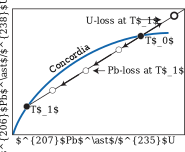
\includegraphics[width=10cm]{../figures/wetherill.png}
\captionof{figure}{`Wetherill' concordia diagram showing concordant
  (filled symbols) and discordant (empty symbols) analyses affected by
  different degrees of Pb (or U) loss \citep[modified
    from][]{allegre2008}.}
  \label{fig:wetherill}
\fi

\section{Detrital geochronology}

Zircon (ZrSiO$_4$) is a common U-Th-bearing accessory mineral in
acidic igneous rocks, which form the main proto-sources of the
siliciclastic sediments. Zircon is a very durable mineral that
undergoes minimal chemical alteration or mechanical
abrasion. Therefore, zircon crystals can be considered time capsules
carrying the igneous and metamorphic history of their
proto-sources. The probability distribution of a representative sample
of zircon U-Pb ages from a detrital population can serve as a
characteristic fingerprint that may be used to trace the flow of sand
through sediment routing systems. As a provenance tracer, zircon U-Pb
data are less susceptible to winnowing effects than conventional
petrographic techniques. Using modern microprobe technology (SIMS and
LA-ICP-MS, see Chapter \ref{sec:mass-specs}), it is quite easy to
date, say, a hundred grains of zircon in a matter of just a few
hours. Due to the robustness of zircons as a tracer of sedimentary
provenance, and the relative ease of dating them, the use of detrital
zircon U-Pb geochronology has truly exploded in recent years. A
literature survey using the keywords `detrital', `zircon', and
`provenance' indicates that the proliferation of detrital zircon
studies has followed an exponential trend, with the number of
publications doubling roughly every five years over the past two
decades. At present, nearly a thousand detrital zircon publications
appear each year.\\

An extensive survey of late Archaean sandstones from the Jack Hills in
Australia have revealed a subpopulation of detrital zircons with
Hadean (4.1-4.2 Ga) U-Pb ages. These are the oldest terrestrial
minerals known to science, predating the oldest igneous rocks by 300
million years.  The isotopic composition of oxygen, hafnium and other
elements in the zircon represents a unique window into the earliest
stages of Earth evolution.  They indicate that liquid water was
present on the surface of our planet early on in its history. This
isotopic evidence is corroborated by the geological observation that
the Hadean zircons are preserved in fluvial deposits.


\chapter{The K-Ar system}
\label{sec:K-Ar}

Potassium has three naturally occurring isotopes: $^{39}$K, $^{40}$K
and $^{41}$K. $^{40}$K is radioactive and undergoes branched decay to
$^{40}$Ca (by electron emission $\lambda_{\beta-} = 4.962 \times
10^{-10} yr^{-1}$) and $^{40}$Ar (by electron capture $\lambda_{e} =
0.581 \times 10^{-10} yr^{-1}$) with a combined half life of 1.248
billion years. The positron emission mechanism mentioned in Chapter
\ref{sec:radioactivity} has an extremely long half life and can
therefore safely be neglected. In addition to $^{40}$Ar, argon has two
more stable isotopes: $^{36}$Ar and $^{38}$Ar. Argon makes up
$\sim$1\% of the terrestrial atmosphere, with a fixed isotopic
composition of $^{40}$Ar/$^{36}$Ar = 298.5 and $^{38}$Ar/$^{36}$Ar =
0.187. The argon contained in K-bearing minerals is made up of a
mixture of radiogenic ($^{40}$Ar$^*$) and non-radiogenic gas
($^{40}$Ar$_\circ$):

\begin{equation}
\begin{array}{rl}
^{40}Ar & = {}^{40}Ar_\circ + {}^{40}Ar^*\\ 
\mbox{where~} {}^{40}Ar^* & =
  \frac{\lambda_e}{\lambda} {}^{40}K \left( e^{\lambda t} - 1 \right)
\end{array}
\label{eq:Ar}
\end{equation}

with $\lambda$ the total decay constant of $^{40}$K ($\lambda =
\lambda_e + \lambda_{\beta-}$ = $5.543 \times 10^{-10} yr^{-1}$).

\section{K-Ar dating}

The $^{40}$K $\rightarrow$ $^{40}$Ar$^*$ decay scheme forms the basis
of the K-Ar geochronometer, with the following age equation:

\begin{equation}
t = \frac{1}{\lambda} \ln\left[ 1 + \frac{\lambda}{\lambda_e}
  \left(\frac{^{40}Ar^*}{^{40}K}\right) \right]
\label{eq:K-Ar}
\end{equation}

Taking into account the `contaminated' (aka `excess' or `inherited')
argon component $^{40}Ar_\circ$ and analysing several cogenetic rocks
or minerals with different K (and therefore $^{40}Ar^*$) contents, an
\emph{isochron} equation can be formed by division through $^{36}$Ar:

\begin{equation}
\frac{^{40}Ar}{^{36}Ar} = \left(\frac{^{40}Ar}{^{36}Ar}\right)_\circ +
\frac{\lambda_e}{\lambda} \frac{^{40}K}{^{36}Ar} \left( e^{\lambda t} - 1 \right)
\label{eq:K-Ar-isochron}
\end{equation}

which can be solved for t. Alternatively, we can simply assume that
all the inherited argon has an atmospheric origin, so that
$({}^{40}Ar/{}^{36}Ar)_\circ = 298.5$.

\section{$^{40}$Ar/$^{39}$Ar dating}
\label{sec:Ar-Ar}

From an analytical perspective, K-Ar dating is a two step
process. Because K (an alkali metal) and Ar (a noble gas) cannot be
measured on the same analytical equipment, they must be analysed
separately on two different aliquots of the same sample.  This
limitation is overcome by the $^{40}$Ar/$^{39}$Ar technique, which is
a clever variation of the K-Ar method. The idea is to subject the
sample to neutron irradiation and convert a small fraction of the
$^{39}$K to synthetic $^{39}$Ar, which has a half life of 269
years. The age equation can then be rewritten as follows:

\begin{equation}
t_x = \frac{1}{\lambda} \ln\left[
1 + J \left(\frac{^{40}Ar^*}{^{39}Ar}\right)_x 
\right]
\label{eq:Ar-Ar}
\end{equation}

where `x' stands for `sample' and J is a constant of proportionality
which encapsulates the efficiency of the $^{39}$K (n,p) $^{39}$Ar
reaction and into which the factor $\lambda/\lambda_e$ is folded as
well.  The J-value can be determined by analysing a standard of known
age t$_s$ which was co-irradiated with the sample:

\begin{equation}
t_s = \frac{1}{\lambda} \ln\left[
1 + J \left(\frac{^{40}Ar^*}{^{39}Ar}\right)_s 
\right]
\label{eq:J}
\end{equation}

In which the subscript `s' stands for `standard'. The great advantage
of equation \ref{eq:Ar-Ar} over \ref{eq:K-Ar} is that all measurements
can be completed on the same aliquot and using a single instrument,
namely a noble gas mass spectrometer, which can analyse extremely
small (down to $\mu$g-sized) samples.\\

The $^{40}$Ar/$^{39}$Ar-method also allows the analyst to investigate
the extent of \emph{argon loss} by means of stepwise heating
experiments.  This is done by degassing the sample under ultra-high
vacuum conditions in a resistance furnace. At low temperatures, the
weakly bound Ar is released, whereas the strongly bound Ar is released
from the crystal lattice at high temperatures until the sample
eventually melts. Plotting the \emph{apparent ages} against the
cumulative fraction of $^{39}$Ar released yields an
$^{40}$Ar/$^{39}$Ar age spectrum (Figure \ref{fig:Ar-Ar}).  If a rock
or mineral has remained closed since its formation, the
$^{40}$Ar/$^{39}$Ar-ratio should remain constant over the course of
the different heating steps, forming an `age plateau'. More complex
(e.g. rising) release spectra, on the other hand, are diagnostic of
complex thermal histories featuring partial argon loss. `saddle'
shaped release spectra are indicative of `excess' argon. The
composition of the inherited argon gas can be determined using a
variant of the isochron method, assuming that all ${}^{36}Ar$ is
inherited:

\begin{equation}
\frac{{}^{40}Ar}{{}^{36}Ar} =
\left(\frac{{}^{40}Ar}{{}^{36}Ar}\right)_\circ +
\frac{{}^{39}Ar}{{}^{36}Ar}\frac{e^{\lambda t} - 1}{J}
\label{eq:Ar-Ar-isochron}
\end{equation}

If the Ar contamination is constant throughout the entire sample, then
the $\frac{^{40}Ar}{^{36}Ar}$-measurements will be arranged along a
linear trend whose slope is a function of $\frac{^{40}Ar^*}{^{39}Ar}$
and, hence, the age.\\

\ifpdf
\ifuclnotes
\begin{figure}[!ht]
  \centering
  \def\svgwidth{.7\textwidth}
  \input{Ar-Ar.pdf_tex}
  \caption{$^{40}$Ar/$^{39}$Ar age spectra obtained by stepwise
    heating of three different K-bearing minerals. Biotite exhibits a
    flat `plateau', indicating a simple history of rapid
    crystallisation and/or cooling. K-feldspar shows a rising age
    spectrum, consistent with a more complex evolution comprising
    multiple growth phases and/or thermal resetting. Finally,
    hornblende shows a `U-shaped' release spectrum in which the first
    heating step releases a large amount of `excess' argon
    \citep[modified from][]{allegre2008}.}
  \label{fig:Ar-Ar}
\end{figure}
\else % end of uclnotes
\begin{figure}[!ht]
\noindent\begin{minipage}[t]{.55\textwidth}
\strut\vspace*{-\baselineskip}\newline
\def\svgwidth{\textwidth}
\input{Ar-Ar.pdf_tex}
\end{minipage}
\begin{minipage}[t]{.45\textwidth}
  \captionof{figure}{$^{40}$Ar/$^{39}$Ar age spectra obtained by stepwise
    heating of three different K-bearing minerals. Biotite exhibits a
    flat `plateau', indicating a simple history of rapid
    crystallisation and/or cooling. K-feldspar shows a rising age
    spectrum, consistent with a more complex evolution comprising
    multiple growth phases and/or thermal resetting. Finally,
    hornblende shows a `U-shaped' release spectrum in which the first
    heating step releases a large amount of `excess' argon
    \citep[modified from][]{allegre2008}.}
  \label{fig:Ar-Ar}
\end{minipage}
\end{figure}
\fi % end of pdf
\else
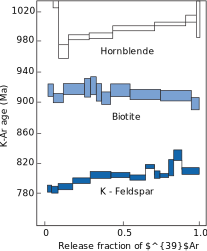
\includegraphics[width=10cm]{../figures/Ar-Ar.png}
  \captionof{figure}{$^{40}$Ar/$^{39}$Ar age spectra obtained by stepwise
    heating of three different K-bearing minerals. Biotite exhibits a
    flat `plateau', indicating a simple history of rapid
    crystallisation and/or cooling. K-feldspar shows a rising age
    spectrum, consistent with a more complex evolution comprising
    multiple growth phases and/or thermal resetting. Finally,
    hornblende shows a `U-shaped' release spectrum in which the first
    heating step releases a large amount of `excess' argon
    \citep[modified from][]{allegre2008}.}
  \label{fig:Ar-Ar}
\fi

\section{Applications}
\label{sec:Ar-applications}

The K-Ar and $^{40}$Ar/$^{39}$Ar-methods are some of the most widely
used geochronometers and important tools in the calibration of the
geologic time scale. The method is applicable to rocks and minerals
$>$ 10$^6$yr. Obviously, younger materials require more careful
treatment of the inherited argon components.

\begin{itemize}
\item{Magmatic rocks:} formation ages can only be obtained for rapidly
  cooled volcanic rocks, using either mineral separates (sanidine,
  biotite, hornblende) or whole rocks. Pyroclastics and obsidian may
  yield reliable ages only if they are unaltered and contain little
  non-radiogenic argon. Plutonic rocks typically cool much slower than
  volcanic rocks and generally yield cooling ages rather than
  formation ages.
\item{Sedimentary rocks:} K-Ar dating of \emph{authigenic} mineral
  phases has often been attempted but remains difficult. Glauconite
  has been used successfully in some cases. Dating detrital minerals
  such as white mica (muscovite, phengite) in fluvial sediments is
  frequently used to study the metamorphic history of the hinterland.
\item{Metamorphic rocks:} pelitic metamorphic rocks tend to be rich in
  K-bearing micas and amphiboles, which can easily be dated with the
  K-Ar and $^{40}$Ar/$^{39}$Ar methods, but require careful
  interpretation. In high grade metamorphic terranes, the apparent
  ages can either reflect the metamorphic crystallisation history or
  the postmetamorphic cooling history. Low grade metamorphic terranes,
  on the other hand, carry a risk of containing inherited argon
  components from previous evolutionary stages.
\end{itemize}


\chapter{Thermochronology}

The temperature sensitivity of the K-Ar system (Section
\ref{sec:K-Ar}) is a characteristic feature not only of this method,
but of a separate class of geochronometers known as
`thermochronometers'.  The most important of these methods are the
U-Th-He \ref{sec:U-Th-He} and fission track \ref{sec:fission-tracks}
techniques, which are becoming increasingly popular as a means of
investigating Earth surface processes.

\section{The U-Th-He method}
\label{sec:U-Th-He}

When U and Th decay to various isotopes of Pb (Section
\ref{eq:UThdecay}), they do so by $\alpha$-emission (Section
\ref{sec:radioactivity}). When $\alpha$ particles acquire electrons,
they become helium atoms. Thus, not only Pb content, but also the He
content increases relative to U and Th through time, forming the basis
of the U-Th-He chronometer:
\begin{equation}
\begin{split}
  \left[^4\mbox{He}\right] = &
  \left[8 \frac{137.818}{138.818} (e^{\lambda_{238}t} - 1) +
    7 \frac{1}{138.818} (e^{\lambda_{235}t} - 1) \right] \mbox{[U]} +\\
  ~ & 6 (e^{\lambda_{232}t} - 1) \mbox{[Th]} +
  0.1499 (e^{\lambda_{147}t} - 1) \mbox{[Sm]}
\end{split}
\label{eq:U-Th-He}
\end{equation}

\noindent where [\textsuperscript{4}He], [U], [Th] and [Sm] are
concentrations in atoms or moles per unit mass or volume.  The values
`8', `7' and `6' refer to the number of $\alpha$-particles produced in
the decay chains of $^{238}$U, $^{235}$U and $^{232}$Th, respectively
(Figure \ref{fig:U-Th-series}), 137.818 is the $^{238}$U/$^{235}$U
ratio of naturally occurring uranium in accessory minerals, and the
last term accounts for the (often negligible) accumulation of helium
by Sm-decay (Section \ref{sec:Sm-Nd}). It was Ernest Rutherford who
first proposed that the U-Th-He decay scheme could be used as an
absolute dating technique, making it the oldest radiometric
chronometer. Early experiments on uraninite (UO$_2$) by Robert John
Strutt (4$^{th}$ Baron Rayleigh) at Imperial College London in 1905
yielded ages that were systematically too young. This was correctly
attributed to the volatile nature of the helium atom, which diffuses
out of most minerals at low temperatures and therefore yields only
\emph{minimum ages}. As a result, the method was largely abandoned
until 1987, when American geochronologist Peter Zeitler realised that
this `leaky' behaviour provided a powerful means of reconstructing the
thermal evolution of rocks and minerals. \\

Let C(x,y,z) be the He-concentration as a function of the spatial
coordinates x, y and z.  The evolution of C with time (t) is given by
the diffusion equation (`Fick's law'):
\begin{equation}
\frac{\partial C}{\partial t} = D \left(
\frac{\partial^2C}{\partial x^2} + \frac{\partial^2C}{\partial y^2} +
\frac{\partial^2C}{\partial z^2}\right)
\label{eq:fick}
\end{equation}

Where D is the `diffusion coefficient', which varies exponentially
with temperature (T) according to the `Arrhenius Law':

\begin{equation}
D = D_\circ e^{-\frac{E_a}{RT}}
\label{eq:Arrhenius}
\end{equation}

with D$_\circ$ the `frequency factor', E$_a$ the `activation energy'
and R the ideal gas constant (8.3144621 J/mol.K). By taking the
logarithm of both sides of Equation \ref{eq:Arrhenius}, we obtain
(Figure \ref{fig:Arrhenius}):

\begin{equation}
\ln(D) = \ln(D_\circ) - \frac{E_a}{RT}
\label{eq:logD}
\end{equation}

Both the frequency factor and the activation energy can be determined
from \emph{diffusion experiments}, in which a He-bearing mineral is
subjected to a step-heating experiment similar to the kind we saw in
the $^{40}$Ar/$^{39}$Ar method (Section \ref{sec:Ar-Ar}).\\

Let us now consider the situation of a mineral which (a) accumulates
He through radioactive decay of U and Th, (b) loses He by thermal
diffusion, and (c) undergoes monotonic cooling at a variable rate
dT/dt. At high temperatures, the He will be lost quickly but as time
progresses, the thermal diffusion becomes increasingly sluggish until
the He is eventually `locked' into the crystal lattice and the isotopic
system is effectively \emph{closed}. If the thermal history is so that
1/T increases linearly with time, then it is possible to calculate an
equivalent `closure temperature' T$_c$. This is known as `Dodson's
equation':

\begin{equation}
\frac{E_a}{RT_c} = \ln\left(\frac{ART_c^2D_\circ/r^2}{E_adT/dt}\right)
\label{eq:Tc}
\end{equation}

where r = is the effective grain size (radius) of the mineral and A is
a geometric factor (55 for a sphere, 27 for a cylinder and 8.7 for a
plane sheet). Thus the U-Th-He age calculated at the end of the
aforementioned thermal history equals that which would have been
obtained if He accumulated linearly since the rock passed through
T$_c$.\\

Although the closure temperature concept is an oversimplification of
reality, it has great intuitive appeal. Consider, for example, a
vertical transect in a rapidly exhuming mountain range. The
\emph{apparent} U-Th-He ages along such a transect are approximately
given by the time elapsed since the respective rocks have passed
through T$_c$. For apatite [Ca$_5$(PO$_4$)$_3$(OH,F,Cl)], this is
$\sim 60^{\circ}C$, which corresponds to a depth (assuming a thermal
gradient of 30$^{\circ}$C/km) of 1.5-2km. Thus, the rocks at the high
elevations along the transect will have passed through T$_c$ before
those collected at the bottom of the transect, and the corresponding
U-Th-He ages will therefore increase with elevation. Moreover, the
rate of increase of age increase with elevation can be used to
estimate the \emph{exhumation rate} of the orogen.

\ifpdf
\ifuclnotes
\begin{figure}[!ht]
  \centering
  \def\svgwidth{.9\textwidth}
  \input{Arrhenius.pdf_tex}
  \caption{`Arrhenius' diagram of three step-heating experiments of
    $^4$He in apatite, showing simple diffusion behaviour in agreement
    with Equation \ref{eq:Arrhenius}. Extrapolating the linear trend
    to geological time scales yields a `closure temperature' of
    $\sim$60$^\circ$C (Equation \ref{eq:Tc}). Modified from
    \citet{braun2006}.}
  \label{fig:Arrhenius}
\end{figure}
\else % end of uclnotes
\begin{figure}[!ht]
\noindent\begin{minipage}[t]{.6\textwidth}
\strut\vspace*{-\baselineskip}\newline
\def\svgwidth{\textwidth}
\input{Arrhenius.pdf_tex}
\end{minipage}
\begin{minipage}[t]{.4\textwidth}
  \captionof{figure}{`Arrhenius' diagram of three step-heating
    experiments of $^4$He in apatite, showing simple diffusion
    behaviour in agreement with Equation
    \ref{eq:Arrhenius}. Extrapolating the linear trend to geological
    time scales yields a `closure temperature' of $\sim$60$^\circ$C
    (Equation \ref{eq:Tc}). Modified from \citet{braun2006}.}
  \label{fig:Arrhenius}
\end{minipage}
\end{figure}
\fi % end of pdf
\else
  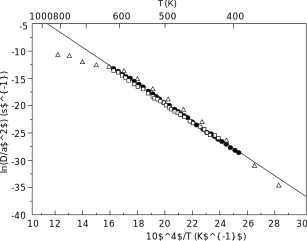
\includegraphics[width=10cm]{../figures/Arrhenius.png}
  \captionof{figure}{`Arrhenius' diagram of three step-heating experiments of
    $^4$He in apatite, showing simple diffusion behaviour in agreement
    with Equation \ref{eq:Arrhenius}. Extrapolating the linear trend
    to geological time scales yields a `closure temperature' of
    $\sim$60$^\circ$C (Equation \ref{eq:Tc}). Modified from
    \citet{braun2006}.}
  \label{fig:Arrhenius}
\fi

\section{Fission tracks}
\label{sec:fission-tracks}

In addition to $\alpha$, $\beta$ and $\gamma$ decay, which form the
basis of the U-Th-Pb (Section \ref{sec:U-Pb}) and U-Th-He (Section
\ref{sec:U-Th-He}) methods, a tiny fraction (1/1,000,000) of the
$^{238}$U atoms decay by \emph{spontaneous fission} (Section
\ref{sec:radioactivity}). In this decay mechanism, the parent nuclide
(i.e., $^{238}$U) decays into two daughter nuclides of roughly equal
mass (e.g., Ba and Kr). These two particles carry a large amount of
energy ($\sim$ 170 MeV) and, having a positive charge, strongly repel
each other. Each of the two fission fragments travels through the
crystal lattice of the host mineral, leaving a trail of damage
behind. Although fission tracks can be directly observed by
transmission electron microscopy (TEM), a more practical approach is
to etch (a polished surface of) the host mineral with acid. This
enlarges the damage zones and makes it possible to count them under an
ordinary petrographic microscope. The volume density $n_s$ (in
cm$^{-3}$) of the fission tracks is given by:
\begin{equation}
n_{s} = \frac{\lambda_f}{\lambda} [^{238}U] \left(e^{\lambda t}-1\right)
\label{eq:Ns}
\end{equation}

where $[^{238}U]$ stands for the volume density the $^{238}$U atoms,
$\lambda_f$ is the fission decay constant
($8.46\times{10}^{-17}$ yr$^{-1}$) and $\lambda$ is the total decay
constant of $^{238}$U ($1.55125\times{10}^{-10}$yr$^{-1}$, see Section
\ref{sec:U-Pb}). The (unobservable) volume density of the tracks is
related to the (observable) surface density $\rho_s$ (in cm$^{-2}$)
by:
\begin{equation}
\rho_s = g_s L n_s
\label{eq:rhos}
\end{equation}

Where g\textsubscript{s} is geometry factor (g\textsubscript{s}=1 if
determined on an internal and g\textsubscript{s}=1/2 on an external
surface) and L is the etchable length of a fission track
($\sim$15$\mu$m). Rearranging Equation \ref{eq:Ns} for time:
\begin{equation}
t = \frac{1}{\lambda}
\ln\left(\frac{\lambda}{\lambda_f}\frac{\rho_s}{[^{238}U] g_s L
}+1\right)
\label{eq:tFT}
\end{equation}

In practice, $[^{238}U]$ is determined by irradiating the (etched)
sample with thermal neutrons in a reactor. This irradiation induces
synthetic fission of $^{235}$U in the mineral (Equation
\ref{eq:235Ufission}). These tracks can be monitored by attaching a
mica detector to the polished mineral surface and etching this monitor
subsequent to irradiation (Figure \ref{fig:EDM}). The surface density
of the induced tracks in the mica detector ($\rho_i$) is a function of
the nuclear cross section of the neutron-induced fission reaction on
$^{235}$U and the neutron fluence in the reactor, both of which are
unknown. A pragmatic solution to this problem is found by irradiating
the sample along with a standard of known age, and lumping all the
unknown parameters together into a calibration factor ($\zeta$), so
that the age of the sample reduces to:
\begin{equation}
t =
\frac{1}{\lambda}\ln\left(1+\frac{g_i}{g_s}\lambda\zeta\rho_d\frac{\rho_s}{\rho_i}\right)
\label{eq:tzeta}
\end{equation}

where $g_s$ = 1, $g_i$ = 1/2 and $\rho_d$ is the surface density of
the induced fission tracks in a dosimeter glass of known (and
constant) U concentration. The latter value is needed to `recycle' the
$\zeta$ value from one irradiation batch to the next, as neutron
fluences might vary through time, or within a sample stack.\\

\ifpdf
\ifuclnotes
\begin{figure}[!ht]
  \centering
  \def\svgwidth{.8\textwidth}
  \input{EDM.pdf_tex}
  \caption{Schematic diagram illustrating the external detector method
    for fission track geochronology \citep[modified
      from][]{galbraith2005}.}
  \label{fig:EDM}
\end{figure}
\else % end of uclnotes
\begin{figure}[!ht]
\noindent\begin{minipage}[t]{.55\textwidth}
\strut\vspace*{-\baselineskip}\newline
\def\svgwidth{\textwidth}
\input{EDM.pdf_tex}
\end{minipage}
\begin{minipage}[t]{.45\textwidth}
  \captionof{figure}{Schematic diagram illustrating the external
    detector method for fission track geochronology \citep[modified
      from][]{galbraith2005}.}
  \label{fig:EDM}
\end{minipage}
\end{figure}
\fi % end of pdf
\else
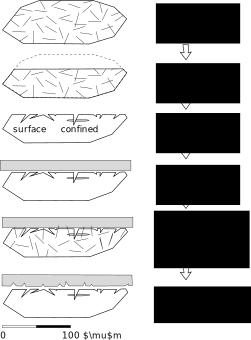
\includegraphics[width=10cm]{../figures/EDM.png}
\caption{Schematic diagram illustrating the external detector method
  for fission track geochronology \citep[modified
    from][]{galbraith2005}.}
  \label{fig:EDM}
\fi

Laboratory experiments have revealed that fission tracks are sensitive
to heat.  For example, it suffices that apatite is heated to
500$^{\circ}$C for 1 hour for all the latent fission tracks to
anneal. Moderate heating shortens the tracks and reduces their surface
density and, hence, the apparent age of the sample. In boreholes, the
apparent fission track age remains constant until a depth is reached
where the ambient temperature is high enough for the tracks to be
reduced in size and number.  This region is called the \emph{Partial
  Annealing Zone} (PAZ). Below the PAZ, no tracks are retained (Figure
\ref{fig:stockli}). The reduction of the surface density of the
spontaneous tracks per unit time can be written as a function of
temperature (T, in Kelvin):

\begin{equation}
\frac{d\rho_s}{dt} = -C \rho_s e^{-E_a/kT}
\label{eq:trackArrhenius}
\end{equation}

where C is a material constant, $E_a$ is the activation energy for
track shortening and k is the Boltzmann constant
(8.616$\times$10$^{-5}$eV/K). Integration of Equation
\ref{eq:trackArrhenius} yields:

\begin{equation}
\ln\left(\frac{\rho_\circ}{\rho}\right) = C~t~e^{-E_a/kT}
\label{eq:lnrho0rho}
\end{equation}

where $\rho_\circ$ is the initial track density prior to
heating. Taking logarithms:

\begin{equation}
\ln(t) = \frac{E_A}{kT} + \ln\left[\ln\left(\frac{\rho_\circ}{\rho}\right)\right] - \ln(C)
\label{eq:lnt}
\end{equation}

For any given \emph{retention coefficient} $\rho_\circ/\rho$, there
exists a linear relationship between ln(t) and 1/T. This is an
\emph{Arrhenius trend} similar to the one described by Equation
\ref{eq:Arrhenius} in the context of U-Th-He thermochronology.  By
extrapolating the Arrhenius diagram to long time scales
($t\sim10^6$yr), it is possible to calculate a `closure temperature'
$T_c$ similar to that which is calculated for the U-Th-He system. For
apatite, T$_c \approx 100^{\circ}C$, whereas for zircon, T$_c \approx
240^{\circ}C$.\\

If a sample has spent some of its time inside the PAZ, then the
subpopulation of its fission tracks formed during that thime will be
shorter than those that subsequently formed above the PAZ. The
probability distribution of the fission track lengths can be
determined by measuring the distance between the two tips of a large
number of (100, say) \emph{horizontally confined} fission tracks under
the optical microscope.  Sophisticated inverse modelling algorithms
have been developed to interpret these length distributions and
extract continuous time-temperature (t-T) paths from them. Such
modelling exercises have become an integral part of modern fission
track studies.

\begin{figure}[!ht]
  \centering
  \ifpdf
  \ifuclnotes
  \def\svgwidth{.9\textwidth}
  \else
  \def\svgwidth{.7\textwidth}
  \fi
  \input{stockli.pdf_tex}
  \else
  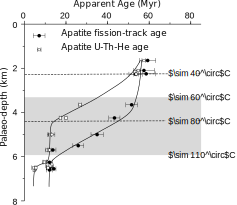
\includegraphics[width=10cm]{../figures/stockli.png}
  \fi
  \caption{Vertical profile of U-Th-He and fission track ages in
    apatite, collected along the footwall of an exhumed normal fault
    block in the White Mountains of eastern California. Samples at the
    highest elevations have resided at shallow depths for up to 55
    Myr. Dashed lines show the extent of the `Partial Retention Zone'
    (PRZ), in which apatite has partially lost its radiogenic
    helium. The grey area indicates the `Partial Annealing Zone',
    where fission tracks have been shortened. At low elevations, young
    ages are observed, indicating rapid exhumation by the normal fault
    at 12 Ma. Additionally, the U-Th-He data show a hint of a second
    exhumation phase at 5 Ma (modified from Stockli, Farley and
    Dumitru, 2000, \textit{Geology} v. 28, no. 11, p. 983-986).}
  \label{fig:stockli}
\end{figure}


\chapter[U-series dating]{U-series disequilibrium methods}
\label{ch:intro2Useries}

In Section \ref{sec:decay-series}, we saw that the
$^{235}$U-$^{207}$Pb and $^{238}$U-$^{206}$Pb decay series generally
reach a state of \emph{secular equilibrium}, in which the activity
(expressed in decay events per unit time) of each intermediate
daughter product is the same, so that:

$$D_n \lambda_n = \cdots  = D_2 \lambda_2 = D_1 \lambda_1 = P \lambda_P$$

as described by Equation \ref{eq:NDnLn}. However, certain natural
processes can disturb this equilibrium situation, such as chemical
weathering, precipitation from a solution, (re-)crystallisation
etc. The leads to two new types of chronometric systems:

\begin{enumerate}
\item An intermediate daughter isotope in the decay series is
  separated from its parent nuclide incorporated into a rock or
  sediment, and decays according to its own half life.
\item A parent nuclide has separated itself from its previous decay
  products and it takes some time for secular equilibrium to be
  re-established.
\end{enumerate}

This idea is most frequently applied to the $^{238}$U-decay series,
notably $^{230}$Th and $^{234}$U. The first type of disequilibrium
dating forms the basis of the $^{234}$U-$^{238}$U and $^{230}$Th
methods (Sections \ref{sec:234238} and \ref{sec:230}). The second
forms the basis of the $^{230}$Th-$^{238}$U method (Section
\ref{sec:230238})

\section{The $^{234}$U-$^{238}$U method}
\label{sec:234238}

The activity ratio of $^{238}$U to its third radioactive daughter
$^{234}$U in the world's oceans is $A(^{234}U)/A(^{238}U)$ $\equiv$
$\gamma_\circ$ $\approx$ 1.15. The slight enrichment of the $^{234}$U
over $^{238}$U is attributed to $\alpha$-recoil of its immediate
parent $^{234}$Th and the fact that $^{234}$U is more `loosely bound'
inside the crystal lattice of the host mineral, because it is
preferentially seated in sites which have undergone radiation
damage. Once the oceanic U is incorporated into the crystal structure
of marine carbonates, the radioactive equilibrium gradually restores
itself with time. The total activity of $^{234}$U is made up of a
component which is supported by secular equilibrium (and equals the
activity of $^{238}U$) and an `excess' component, which decays with
time:

\begin{equation}
A(^{234}U) = A(^{238}U) + A(^{234}U)^x_\circ e^{-\lambda_{234}t} 
\label{eq:A234}
\end{equation}

where $A(^{234}U)^x_\circ$ is the initial amount of excess $^{234}$U
and $\lambda_{234}$ = 2.8234 $\times$ 10$^{-6}$ yr$^{-1}$ (t$_{1/2}$ =
245.5 kyr). Let $A(^{234}U)_\circ$ be the initial total $^{234}$U
activity. Then:

\begin{equation}
A(^{234}U) = A(^{238}U) + \left[A(^{234}U)_\circ - A(^{238}U) \right] e^{-\lambda_{234}t} 
\label{eq:A234b}
\end{equation}

Dividing by A($^{238}$U):

\begin{equation}
\frac{A(^{234}U)}{A(^{238}U)} = 1 + [ \gamma_\circ - 1 ] e^{-\lambda_{234}t} 
\label{eq:A234A238}
\end{equation}

Which can be solved for $t$ until about 1 Ma.

\section{The $^{230}$Th method}
\label{sec:230}

U and Th are strongly incompatible elements. This causes chemical
fractionation and disturbs the secular equilibrium of the $^{238}$U
decay series in young volcanic rocks. It is commonly found that the
activity ratio $A(^{230}Th)/A(^{238}U)$ $>$ 1. As expected, the
secular equilibrium between $^{234}$U and $^{238}$U is not disturbed
by chemical fractionation, so that $A(^{234}U)/A(^{238}U)$ = 1. The
total $^{230}$Th activity is given by:

\begin{equation}
A(^{230}Th) = A(^{230}Th)_\circ e^{-\lambda_{230}t} + A(^{238}U)(1-e^{-\lambda_{230}t})
\label{eq:A230}
\end{equation}

where $A(^{230}Th)_\circ$ is the initial amount of $^{230}$Th at the
time of crystallisation and $A(^{238}U)=A(^{234}U)$ due to secular
equilibrium of the U isotopes. Thus, the first term of Equation
\ref{eq:A230} increases with time from 0 to A($^{238}$U) while the
second term decreases from $A(^{230}Th)_\circ$ to 0. Dividing by
$A(^{232}Th)$ yields a linear relationship between
$A(^{230}Th)/A(^{232}Th)$ and $A(^{238}U) / A(^{232}Th)$:

\begin{equation}
\frac{A(^{230}Th)}{A(^{232}Th)} = \frac{A(^{230}Th)_\circ}{A(^{232}Th)} e^{-\lambda_{230}t} + 
\frac{A(^{238}U)}{A(^{232}Th)}(1-e^{-\lambda_{230}t})
\label{eq:230232}
\end{equation}

This forms an isochron with slope ($1-e^{-\lambda_{230}t}$), from
which the age $t$ can be calculated. This method is applicable to
volcanic rocks and pelitic ocean sediments ranging from 3ka to 1Ma.

\section{The $^{230}$Th-U method}
\label{sec:230238}

Uranium is significantly more soluble in water than Th. As a result,
the intermediate daughter $^{230}$Th is largely absent from sea
water. Thus, lacustrine and marine carbonate rocks contain some U but
virtually no Th at the time of formation. The $^{230}$Th activity
increases steadily with time as a result of $^{234}$U decay. The total
$^{230}$Th activity consists of a growing component $A(^{230}Th)^s$
that is in secular equilibrium with $^{238}U$ and a shrinking
component $A(^{230}Th)^x$ of `excess' $^{230}$Th produced by the
surplus of $^{234}$U commonly found in ocean water (see section
\ref{sec:234238}):

\begin{align}
~ & A(^{230}Th) =  A(^{230}Th)^s + A(^{230}Th)^x \label{eq:230total}\\
\mbox{with:~} & A(^{230}Th)^s = A(^{238}U) (1-e^{-\lambda_{230}t}) \label{eq:230s}\\
\mbox{and:~} & A(^{230}Th)^x = \frac{\lambda_{230}}{\lambda_{230}-\lambda_{234}} 
A(^{234}U)_\circ^x\left(e^{-\lambda_{234}t}-e^{-\lambda_{230}t}\right) \label{eq:230x}
\end{align}

In which the expression for $A(^{230}Th)^x$ follows from Equation
\ref{eq:ND1} and $A(^{234}U)_\circ^x$ denotes the initial amount of
excess $^{234}$U activity (as in Section \ref{sec:234238}). Taking
into account that $A(^{234}U)_\circ^x = A(^{234}U)_\circ -
A(^{238}U)$, and dividing by $A(^{238}U)$, we obtain:

\begin{equation}
\frac{A(^{230}Th)^x}{A(^{238}U)} = \frac{\lambda_{230}}{\lambda_{230}-\lambda_{234}} (\gamma_\circ-1)
\left(e^{-\lambda_{234}t}-e^{-\lambda_{230}t}\right)
\label{eq:230238x}
\end{equation}

in which $\gamma_\circ \equiv A(^{234}U)/A(^{238}U)$ as defined in
Section \ref{sec:234238}. The formation age of the carbonate can be
calculated by substituting Equations \ref{eq:230s} and \ref{eq:230238x}
into \ref{eq:230total} and solving for $t$. 

\begin{equation}
  \frac{A(^{230}Th)}{A(^{238}U)} = 1 - e^{-\lambda_{230}t} +
  \frac{\lambda_{230}}{\lambda_{230}-\lambda_{234}} (\gamma_\circ-1)
\left(e^{-\lambda_{234}t}-e^{-\lambda_{230}t}\right)
\label{eq:230238}
\end{equation}

If $\gamma_\circ = 1$ (i.e., the water is in secular equilibrium for
U), then Equation \ref{eq:230total} simplifies to:

\begin{equation}
\frac{A(^{230}Th)}{A(^{238}U)} = 1-e^{-\lambda_{230}t}
\label{eq:230238b}
\end{equation}

If $\gamma_\circ \neq 1$, Equation \ref{eq:230238b} yields ages that
are systematically too old (if $\gamma_\circ > 1$) or too young (if
$\gamma_\circ < 1$).


\chapter{Error propagation}
\label{ch:error-propagation}

All the methods and equations presented thus far have assumed that all
parameters are either known or measured with infinite precision. In
reality, however, the analytical equipment used to measure isotopic
compositions, elemental concentrations and radioactive half-lives is
not perfect.  It is crucially important that we quantify the resulting
analytical uncertainty before we can reliably interpret the resulting
ages.\\

For example, suppose that the extinction of the dinosaurs has been
dated at 65 Ma in one field location, and a meteorite impact has been
dated at 64 Ma elsewhere.  These two numbers are effectively
meaningless in the absence of an estimate of precision. Taken at face
value, the dates imply that the meteorite impact took place 1 million
years after the mass extinction, which rules out a causal relationship
between the two events. If, however, the analytical uncertainty is
significantly greater than 1 Myr (e.g. 64 $\pm$ 2 Ma and 65 $\pm$ 2
Ma), then such of a causal relationship remains very plausible.

\section{Some basic definitions}
\label{sec:summarystatistics}

Suppose that our geochronological age ($t$) is calculated as a function
($f$) of some measurements ($x$ and $y$):

\begin{equation}
t = f(x,y)
\label{eq:tfxy}
\end{equation}

Suppose that we have performed a large number ($n$) of replicate
measurements of $x$ and $y$:

\begin{equation}
\left\{
\begin{array}{rl}
x = & \{x_1, x_2, \cdots, x_i, \cdots, x_n\} \\
y = & \{y_1, y_2, \cdots, y_i, \cdots, y_n\}
\end{array}
\right.
\label{eq:xy}
\end{equation}

It is useful to define the following \emph{summary statistics}:

\begin{enumerate}
\item The mean:
\begin{equation}
\left\{
\begin{array}{rl}
\overline{x} \equiv & \frac{1}{n} \sum_{i=1}^{n} x_i\\
\overline{y} \equiv & \frac{1}{n} \sum_{i=1}^{n} y_i
\end{array}
\right.
\label{eq:mean}
\end{equation}

is a useful definition for the `most representative' value of $x$ and
$y$, which can be plugged into Equation~\ref{eq:tfxy} to calculate the
`most representative' age.

\item The variance:
\begin{equation}
\left\{
\begin{array}{rl}
s[x]^2 \equiv & \frac{1}{n-1} \sum_{i=1}^{n} (x_i-\overline{x})^2\\
s[y]^2 \equiv & \frac{1}{n-1} \sum_{i=1}^{n} (y_i-\overline{y})^2
\end{array}
\right.
\label{eq:variance}
\end{equation}

with $s[x]$ and $s[y]$ the `standard deviations', is used to quantify
the amount of dispersion around the mean.

\item The covariance:
\begin{equation}
s[x,y] \equiv \frac{1}{n-1} \sum_{i=1}^{n} (x_i-\overline{x})(y_i-\overline{y})
\label{eq:covariance}
\end{equation}

quantifies the degree of correlation between variables $x$ and $y$.
\end{enumerate}

$\overline{x}$, $\overline{y}$, $s[x]^2$, $s[y]^2$ and $s[x,y]$ can
all be estimated from the input data $(x,y)$. These values can then be
used to infer $s[t]^2$, the variance of the calculated age $t$, a
process that is known as `error propagation'. To this end, recall the
definition of the variance (Equation \ref{eq:variance}):

\begin{equation}
s[t]^2 \equiv \frac{1}{n-1} \sum_{i=1}^{n} (t_i-\overline{t})^2
\label{eq:vart}
\end{equation}

We can estimate $(t_i-\overline{t})$ by differentiating Equation
\ref{eq:tfxy}:

\begin{equation}
t_i - \overline{t} = (x_i-\overline{x}) \frac{\partial f}{\partial x} +
(y_i-\overline{y}) \frac{\partial f}{\partial y}
\label{eq:ti-t}
\end{equation}

Plugging Equation \ref{eq:ti-t} into \ref{eq:vart}, we obtain:

\begin{align}
s[t]^2 & = \frac{1}{n-1} \sum_{i=1}^{n} \left[
(x_i-\overline{x}) \left(\frac{\partial f}{\partial x}\right) +
(y_i-\overline{y}) \left(\frac{\partial f}{\partial y}\right) \right]^2 \label{eq:s2t1}\\
~ & = s[x]^2 \left(\frac{\partial f}{\partial x}\right)^2 +
s[y]^2 \left(\frac{\partial f}{\partial y}\right)^2 +
2~s[x,y] \frac{\partial f}{\partial x} \frac{\partial f}{\partial y} \label{eq:s2t}
\end{align}

This is the general equation for the propagation of uncertainty with
two variables, which is most easily extended to more than two
variables by reformulating Equation \ref{eq:s2t} into a matrix form:

\begin{equation}
s[t]^2 = 
\left[
\begin{array}{@{}c@{~}c@{}}
\frac{\partial t}{\partial x}&\frac{\partial t}{\partial y}
\end{array}
\right]
\left[
\begin{array}{@{}c@{~}c@{}}
s[x]^2 & s[x,y]\\
s[x,y] & s[y]^2
\end{array}
\right]
\left[
\begin{array}{@{}c@{}}
\frac{\partial t}{\partial x} \\
\frac{\partial t}{\partial y}
\end{array}
\right]
\label{eq:s2tmatrix}
\end{equation}

where the innermost matrix is known as the \emph{variance-covariance}
matrix and the outermost matrix (and its transpose) as the
\emph{Jacobian matrix}.  Let us now apply this equation to some simple
functions.

\section{Examples}

Let $x$ and $y$ indicate measured quantities associated with
analytical uncertainty.  And let $a$ and $b$ be some error free
parameters.

\begin{enumerate}
\item{addition:}
\begin{align}
& t = a x + b y \Rightarrow \frac{\partial t}{\partial x} = a, 
\frac{\partial t}{\partial y} = b \nonumber\\
& \Rightarrow s[t]^2 = a^2 s[x]^2 + b^2 s[y]^2 + 2ab~s[x,y]
\label{eq:addition}
\end{align}

\item{subtraction:}
\begin{equation}
t = a x - b y \Rightarrow
s[t]^2 = a^2 s[y]^2 + b^2 s[y]^2 - 2ab~s[x,y]
\label{eq:subtraction}
\end{equation}

\item{multiplication:}
\begin{align}
& t = a x y \Rightarrow \frac{\partial t}{\partial x} = a y, 
\frac{\partial t}{\partial y} = ax \nonumber\\
& \Rightarrow s[t]^2 = (ay)^2 s[x]^2 + (ax)^2 s[y]^2 + 2a^2 xy~s[x,y] \nonumber\\
& \Rightarrow \left(\frac{s[t]}{t}\right)^2 = \left(\frac{s[x]}{x}\right)^2 + 
  \left(\frac{s[y]}{y}\right)^2 + 2 \frac{s[x,y]}{x y}
\label{eq:multiplication}
\end{align}

\item{division:}
\begin{equation}
t = a \frac{x}{y} \Rightarrow
\left(\frac{s[t]}{t}\right)^2 = \left(\frac{s[x]}{x}\right)^2 + 
  \left(\frac{s[y]}{y}\right)^2 - 2 \frac{s[x,y]}{x y}
\label{eq:division}
\end{equation}

\item{exponentiation:}
\begin{equation}
t = a~e^{bx} \Rightarrow \frac{\partial f}{\partial x} = ab~e^{bx} 
\Rightarrow s[t]^2 = (b t)^2 s[x]^2
\label{eq:exponentiation}
\end{equation}

\item{logarithms:}
\begin{equation}
t = a~\ln(bx) \Rightarrow \frac{\partial f}{\partial x} = \frac{a}{x}
\Rightarrow s[t]^2 = a^2 \left(\frac{s[x]}{x}\right)^2
\label{eq:logarithms}
\end{equation}

\item{power:}
\begin{equation}
  t = a x^b \Rightarrow \frac{\partial f}{\partial x} = b \frac{a
    x^b}{x} \Rightarrow \left(\frac{s[t]}{t}\right)^2 =
  b^2\left(\frac{s[x]}{x}\right)^2
\label{eq:power}
\end{equation}

\end{enumerate}

\section{Accuracy vs. precision}

Recall the definition of the arithmetic mean (Equation \ref{eq:mean}):

$$\overline{x} \equiv \frac{1}{n} \sum_{i=1}^{n} x_i$$

Applying the equation for the error propagation of a sum (Equation
\ref{eq:addition}):

\begin{equation}
s[\overline{x}]^2 = \frac{1}{n} \sum_{i=1}^{n} s[x_i]^2 =
\frac{s[x]^2}{n}
\label{eq:varianceofthemean}
\end{equation}

where we assume that all $n$ measurements were done
\emph{independently}, so that $cov(x_i,x_j)=0 \forall i, j$.  The
standard deviation of the mean is known as the \underline{standard
  error}:

\begin{equation}
s[\overline{x}] = \frac{s[x]}{\sqrt{n}}
\label{eq:standarderror}
\end{equation}

This means that the standard error of the mean monotonically decreases
with the square root of sample size. In other words, we can
arbitrarily increase the \emph{precision} of our analytical data by
acquiring more data. However, it is important to note that the same is
generally not the case for the \emph{accuracy} of those data. The
difference between precision and accuracy is best explained by a darts
board analogy:\\

\noindent
\begin{minipage}{\textwidth}
  \centering
  \ifpdf
  \def\svgwidth{\textwidth}
  \input{bullseye.pdf_tex}
  \else
  
\includegraphics[width=10cm]{../figures/bullseye.png}
  \fi
\end{minipage}

\bigskip

Whereas the analytical precision can be computed from the data using
the error propagation formulas introduced above, the only way to get a
grip on the accuracy is by analysing another sample of independently
determined age. Such test samples are also known as `secondary
standards'.

\ifpdf
\ifuclnotes
\begin{figure}[!ht]
  \centering
  \def\svgwidth{\textwidth}
  \input{covariance.pdf_tex}
  \caption{Four datasets of 100 random numbers (black dots) which have
    the same means (white squares) but different (co-)variance
    structures. The marginal distributions of the $x$ and $y$ variables
    are shown as `bell curves' on the top and right axis of each
    plot.}
  \label{fig:covariance}
\end{figure}
\else % end of uclnotes
\begin{figure}[!ht]
  \noindent\begin{minipage}[t]{.7\textwidth}
\strut\vspace*{-\baselineskip}\newline
\def\svgwidth{\textwidth}
\input{covariance.pdf_tex}
\end{minipage}
\begin{minipage}[t]{.3\textwidth}
  \captionof{figure}{Four datasets of 100 random numbers (black dots) which have
    the same means (white squares) but different (co-)variance
    structures. The marginal distributions of the $x$ and $y$ variables
    are shown as `bell curves' on the top and right axis of each
    plot.}
  \label{fig:covariance}
\end{minipage}
\end{figure}
\fi % end of pdf
\else
\includegraphics[width=10cm]{../figures/covariance.png}
  \captionof{figure}{Four datasets of 100 random numbers (black dots) which have
    the same means (white squares) but different (co-)variance
    structures. The marginal distributions of the $x$ and $y$ variables
    are shown as `bell curves' on the top and right axis of each
    plot.}
  \label{fig:covariance}
\fi


\chapter{Exercises}
\label{ch:exercises}

\begin{enumerate}

\item If helium ions (mass number = 4) are accelerated with a voltage
  of 10 kV in a mass spectrometer, at what speed are they emitted from
  the source? Recall that 1 atomic mass unit (amu) = 1.66 $\times$
  10$^{-27}$ kg and the elementary charge is 1.602 $\times$ 10$^{-19}$
  C. \rotatebox[origin=c]{180}{[Answer: 695 km/s]}

\item We are trying to estimate the Rb concentration in a rock for the
  purpose of whole rock Rb-Sr dating. To this end, we use a spike with
  a Rb concentration of 7.5 ppm containing 99.4\% $^{87}$Rb and 0.6\%
  $^{85}$Rb (these are atomic abundances). We mix 3.5g of the spike
  with 0.25g of sample dissolved in 50g. The $^{87}$Rb/$^{85}$Rb-ratio
  of the mixture is 1.55, as measured by mass spectrometry. What is
  the Rb concentration in ppm? Note that natural Rb comprises of
  27.825\% $^{87}$Rb and 72.165\% $^{85}$Rb.  
  \rotatebox[origin=c]{180}{[Answer: 120 ppm]}

\item A biotite contains 465ppm Rb and 30ppm Sr with a
  $^{87}$Sr/$^{86}$Sr-ratio of 2.50.  Given an initial
  $^{87}$Sr/$^{86}$Sr-ratio of 0.7035, what is the age of the biotite?
  Natural Rb has an atomic mass of 85.4678 and comprises 72.165\%
  $^{85}$Rb and 27.825\% $^{87}$Rb, which has a half life of t$_{1/2}$
  = 48.8 Gyr. Sr has an atomic mass of 87.62. Its non-radiogenic
  isotopes occur with the following abundances: $^{84}$Sr/$^{86}$Sr =
  0.056584 and $^{86}$Sr/$^{88}$Sr = 0.1194.
  \rotatebox[origin=c]{180}{[Answer: 2.36 Ga]}

\item Consider a zircon with the following composition: U = 792.1 ppm,
  Th = 318.6 ppm, Pb = 208.2 ppm. Atomic masses for U, Th and Pb in
  the zircon are 238.04, 232.04 and 205.94, respectively. The isotopic
  composition of the Pb is as follows: $^{204}$Pb = 0.048\%,
  $^{206}$Pb = 80.33\%, $^{207}$Pb = 9.00\%, $^{208}$Pb =
  10.63\%. Assume the following initial Pb composition: 204 : 206 :
  207 : 208 = 1.00 : 16.25 : 15.51 : 35.73. The decay constants for
  $^{238}$U, $^{235}$U and $^{232}$Th are given in Section
  \ref{sec:U-Pb}. $^{238}$U/$^{235}$U = 137.818. Calculate the
  $^{206}$Pb/$^{238}$U, $^{207}$Pb/$^{235}$U, $^{208}$Pb/$^{232}$Th
  and $^{207}$Pb/$^{206}$Pb-age of the zircon. Give an account of its
  formation history. \\ \rotatebox[origin=c]{180}{[Answer: 1.405,
      1.523, 1.284 and 1.689 Ga]}

\item A biotite was separated from granite and dated with the K-Ar
  method. The analytical data are as follows: K$_2$O = 8.45 weight \%,
  radiogenic $^{40}$Ar = 6.015 $\times$ 10$^{-10}$ mol/g.  What is the
  K-Ar age of the biotite? The atomic mass of K is 39.098 (and oxygen
  15.9994), with an isotopic composition that comprises 93.258\%
  $^{39}$K, 6.730\% $^{41}$K and 0.01167\% $^{40}$K, which has a
  half-life of t$_{1/2}$ = 1.248 Gyr. Recall that only 10.72\% of the
  $^{40}$K decays to $^{40}$Ar, with the remaining 89.28\% turning
  into $^{40}$Ca. \rotatebox[origin=c]{180}{[Answer: 47.7 Ma]}

\item Consider a biotite with a conventional K-Ar age of 384Ma. A
  $^{40}$Ar/$^{39}$Ar step-heating experiment yields the following
  data:

\begin{centering}
\begin{tabular}{c@{~}|@{~}c@{~}c@{~}c@{~}c@{~}c@{~}c@{~}c}
\% $^{39}$Ar released & 7 & 15 & 20 & 25 & 35 & 70 & 100\\
$^{40}$Ar$^*/^{39}$Ar & 2.27 & 4.97 & 6.68 & 9.58 & 10.25 & 10.10 & 10.26 \\
\end{tabular}
\end{centering}

The analysis was done using a co-irradiated 1.062 Ga biotite age
standard yielding a $^{40}$Ar$^*$/$^{39}$Ar-ratio of 27.64.  Construct
the $^{40}$Ar/$^{39}$Ar age spectrum and use this to comment on the
thermal history of the host rock. t$_{1/2}$($^{40}$Ar) = 1.248
Gyr.\\ \rotatebox[origin=c]{180}{[Answer: 115, 243, 319, 442, 470, 463
    and 470 Ma]}

\item How many cm$^3$ of helium does a rock weighing 1 kg and
  containing 2 ppm of uranium produce after 1 billion years? The molar
  volume of an ideal gas is 22.414 litres. Uranium has an atomic mass
  of 238.04 with $^{238}$U/$^{235}$U = 137.818. Decay constants of U
  are given in Section \ref{sec:U-Pb}.
\rotatebox[origin=c]{180}{[Answer: 0.27 cm$^3$]}

\item Repeated analysis of the Fish Canyon zircon age standard (t=27.8
  Ma) yields the following fission track data:
  
\begin{centering}
\begin{tabular}{ccc}
$\rho_s$ & $\rho_i$ & $\rho_d$ \\
($\times$10$^5$cm$^{-2}$) & ($\times$10$^6$cm$^{-2}$) & ($\times$10$^5$cm$^{-2}$)\\
\hline
36.56 & 6.282 & 2.829 \\
38.97 & 7.413 & 3.313 \\
56.53 & 7.878 & 2.457 \\
41.05 & 8.578 & 3.485 \\
45.87 & 6.985 & 2.482
\end{tabular}
\end{centering}

Compute the average $\zeta$-calibration factor and use this to
calculate the zircon fission track ages of the following rocks:

\begin{centering}
\begin{tabular}{r@{~}c@{~}c@{~}c}
~ & $\rho_s$ & $\rho_i$ & $\rho_d$ \\
~ & ($\times$10$^5$cm$^{-2}$) & ($\times$10$^6$cm$^{-2}$) & ($\times$10$^5$cm$^{-2}$)\\
\hline
Tardree rhyolite & 60.49 & 2.66 & 1.519 \\
Bishop tuff & 6.248 & 1.299 & 0.081 \\
\end{tabular}
\end{centering}

The half-life of $^{238}$U is t$_{1/2}$ = 4.47 Gyr.\\
\rotatebox[origin=c]{180}{[Answer: Tardree -- 57 Ma; Bishop -- 643 ka]}

\item A fossil mollusc has been found in a Quaternary beach formation
  and its activity ratio measured as A($^{230}$Th) / A($^{238}$U) =
  0.6782. Determine the age of the fossil assuming that $\gamma_\circ$
  = 1.15 and given that the half lives of $^{230}$Th and $^{234}$U are
  75,380 and 245,500 years,
  respectively. \rotatebox[origin=c]{180}{[Answer: 100kyr]}

\end{enumerate}


\input{intro2manualpracticals.tex}

\section{Introduction to \texttt{R}}
\label{sec:R}

A number of different graphical user interfaces (GUIs) are available
to interact with \texttt{R}. The most popular of these are
\texttt{Rgui}, \texttt{RStudio}, \texttt{RCommander} and
\texttt{Tinn-R}.

\begin{enumerate}
  \item Starting these applications or running \texttt{R} in a text
    terminal presents the user with a command line prompt. Anything
    that is typed after the \texttt{>} symbol will be evaluated
    immediately. Thus, we can use \texttt{R} as a calculator:

\begin{console}
> 1 + 1
> sqrt(2)
> exp(log(10))
> 31 %% 14
\end{console}

\item Alternatively, code can also be saved as text (using a built-in text
  editor) and saved as \texttt{mycode.R}, say. This code can then be
  copied and pasted at the command line prompt. Or it can be called from
  the command line using the \texttt{source()} function:

\begin{console}
> source('mycode.R')
\end{console}

\item In the remainder of this tutorial, we will assume that your code is
  run from a text file unless explicitly stated otherwise. The
  \texttt{\#}~symbol marks the beginning of a comment.  \texttt{R}
  ignores anything that follows it:

\begin{script}
# The arrow symbol is used to assign a value to a
# variable. Note that the arrow can point both ways:
foo <- 2
4 -> bar
print(foo*bar)

# Defining a vector of multiple values:
myvec <- c(0,1,2,3,4,5)
# or, equivalently:
myvec <- seq(0,5)
# or
myvec <- seq(from=0,to=5,by=1)
# or
myvec <- 0:5

# Turn myvec into a 2x3 matrix:
mymat <- matrix(myvec,nrow=2)

# Accessing one or more items from a vector or matrix:
x <- myvec[3]
y <- myvec[1:3]
z <- mymat[1,2:3]

# Change the 2nd value in mymat's 3rd column to 10:
mymat[2,3] <- 10

# Change the entire second column of mymat to -1:
mymat[,2] <- -1

# Transpose of a matrix:
flipped <- t(mymat)

# Element-wise multiplication (*) 
# vs. matrix multiplication (%*%):
rectangle <- mymat * mymat
square <- mymat %*% flipped
\end{script}

\item Lists are used to store more complex data objects:

\begin{script}
mylist <- list(v=myvec,m=mymat,nine=9)
\end{script}

The three components of \texttt{mylist} can be accessed in a number of
equivalent ways. For example, the first item (\texttt{v}) of
\texttt{mylist} can be accessed either as \verb|mylist$v|, as
\verb|mylist[[1]]| or as \verb|mylist[['v']]|.\\

Data frames are list-like tables:

\begin{script}
myframe <- data.frame(period=c('Cz','Mz','Pz','PC'),
                      SrSr=c(0.708,0.707,0.709,0.708),
                      fossils=c(TRUE,TRUE,TRUE,FALSE))
\end{script}

You can access the items in the data frame \texttt{myframe} either
like a list (e.g. \verb|myframe$period|) or like a matrix
(\verb|myframe[,'period']|):

\item If you want to learn more about a function, type \texttt{help()} or
\texttt{?} at the command line prompt:

\begin{console}
> help(c)
> ?matrix
\end{console}

\item In addition to \texttt{R}'s built-in functions, you can also define
  your own:

\begin{script}
cube <- function(n){
    return(n^3)
}

# Using this function to take the cube of 3:
c3 <- cube(3)

# Conditional statement:
toss <- function(){
    if (runif(1)>0.5){ # runif(n) draws n random 
        print("head")  # numbers between 0 and 1
    } else {
        print("tail")
    }
}

# Use a for loop to toss 10 virtual coins:
for (i in 1:10) {
    toss()
}
\end{script}

\item The purpose of the practical exercises in
  Sections~\ref{sec:U-Pb-R}-\ref{sec:FT-R} is to process datasets
  contained in external data files. For this you will need to be able
  to navigate through your file system and load the necessary files:

\begin{console}
> ls()          # list all the variables
> rm(list=ls()) # clear the current workspace
> getwd()       # get the current working directory
> setwd("path_to_a_valid_directory")
\end{console}

\item Use the above commands to navigate to the directory containing the
file named \texttt{RbSr.csv}. Then read this file into memory:

\begin{script}
RbSr <- read.csv("RbSr.csv",header=TRUE)
\end{script}

Type \texttt{names(RbSr)} or \texttt{colnames(RbSr)} at the command
prompt to list the variable names (column headers) contained in this
dataset.

\item Let us now perform an isochron regression
  (Section~\ref{sec:Rb-Sr}) through these Rb-Sr data: \label{itm:lm}

\begin{script}[firstnumber=2]
# Plot Sr87Sr86 against Rb87Sr86:
plot(RbSr[,'Rb87Sr86'],RbSr[,'Sr87Sr86'],type="p")

# fit a linear model to the data
fit <- lm(Sr87Sr86 ~ Rb87Sr86, data = RbSr)
\end{script}

\item \texttt{fit} is a `list' object. Type \texttt{str(fit)} at the
  command prompt to see its structure. One of its items is
  \verb|fit$coefficients|, which contains the slope and the intercept
  of the linear fit. Alternatively, we can also access these values
  using the \texttt{coef()} function. The following code uses this
  function to calculate the isochron age:

\begin{script}[firstnumber=7]
# define the 87Rb decay constant (in Ma-1):
lam87 <- 1.3972e-5 # according to Villa et al. (2015)
# compute the age from the slope:
tRbSr <- log(1 + coef(fit)[2])/lam87

# add the best fit line to the existing plot:
abline(fit)
# label with the isochron age: 
title(tRbSr)
\end{script}

\item\label{it:installingIsoplotR} One of the most powerful features
  of \texttt{R} is the availability of thousands of `packages'
  providing additional functionality to the built-in functions.  For
  example, let us download and install the \texttt{IsoplotR} package
  from the `Comprehensive R Archive Network' (CRAN):

\begin{console}
> install.packages('IsoplotR')
\end{console}

\item We can use \texttt{IsoplotR} to redo the isochron regression
  exercise using a more rigorous weighted regression algorithm that
  takes into account the analytical uncertainties in both the
  \textsuperscript{87}Sr/\textsuperscript{86}Sr- and
  \textsuperscript{87}Rb/\textsuperscript{86}Sr-ratios:

\begin{script}
# load the functionality of the IsoplotR package:
library('IsoplotR')

# load the data (see ?read.data for details):
RbSr2 <- read.data('RbSr.csv',method='Rb-Sr',format=1)

# compute and plot the isochron diagram:
isochron(RbSr2)
\end{script}

Even though \texttt{IsoplotR} is powerful, convenient, and popular, we
will not use it in the remainder of these notes. Instead, we will
carry out all our calculations in base \texttt{R} because this will
give you a more fundamental understanding of geochronology.
\end{enumerate}


\section{U-Th-Pb data reduction}
\label{sec:U-Pb-R}

You are supplied with two data files that were produced by the
quadrupole laser ablation ICP-MS system at UCL's London Geochronology
Centre. At the time of the analysis, this instrument could not resolve
$^{204}$Pb from the isobaric interference at $^{204}$Hg. Therefore, it
is not possible to apply a common lead correction as explained in
Section \ref{sec:U-Pb}. However, this does not cause any major issues
to us because:

\begin{enumerate}
\item The mineral analysed is zircon, which incorporates very little
  common Pb in its crystal structure during crystallisation.
\item The ages are sufficiently old for the radiogenic Pb to dominate
  the common Pb component by orders of magnitude.
\end{enumerate}

In this exercise, we will use standard-sample bracketing
(Section~\ref{sec:bracketing}) to process some raw mass spectrometer
data in \texttt{R} \ifuclnotes or \texttt{Matlab}\fi:

\begin{enumerate}
\item Load the input files {\tt 91500.csv} (sample) and {\tt GJ1.csv}
  (standard) into memory.
\item Plot the $^{238}$U signal against time. The resulting curve
  consists of three segments: (i) the first 20 seconds record the
  background (`blank') signal of the ICP-MS, measured while the laser
  was switched off; (ii) 20~seconds into the run, the laser is turned
  on and the ions arrive in the ICP-MS; (iii) After the signal has
  ramped up quickly, it slowly drops over time as the laser goes out
  of focus whilst drilling deeper into the sample. This is the
  `signal'.
\item Compute the arithmetic mean U and Pb blank (measurements before
  20 seconds), and subtract them from the signal (measurements after
  25 seconds). Do this for both the sample and the standard.  You will
  get two times four vectors, for $^{206}$Pb, $^{207}$Pb, $^{235}$U
  and $^{238}$U.
\item Use the four blank corrected signal vectors to form two pairs of
  $^{206}$Pb/$^{238}$U and $^{207}$Pb/$^{235}$U vectors.
\item Take the arithmetic mean of the $^{206}$Pb/$^{238}$U and
  $^{207}$Pb/$^{235}$U ratio vectors. You will now have two pairs of
  numbers representing the \emph{measured} $^{206}$Pb/$^{238}$U and
  $^{207}$Pb/$^{235}$U ratios for the sample and the standard.
\item Given that GJ-1 has a known age of 600.4 Ma, what are its
  \emph{expected} $^{206}$Pb/$^{238}$U, and $^{207}$Pb/$^{235}$U
  ratios? Is there a significant difference between the measured and
  the expected ratios? What could be causing this?
\item\label{it:corr} Calculate a correction factor by dividing the
  expected GJ-1 ratios by the measured values.
\item\label{it:atomicUPb} Apply the correction factor calculated in
  step~\ref{it:corr} to the measured ratios for sample 91500. This
  gives us two estimated atomic $^{206}$Pb/$^{238}$U and
  $^{207}$Pb/$^{235}$U ratios.
\item What is the age of 91500?
\item Can you plot the results on a Wetherill concordia diagram?
\end{enumerate}


\section{$^{40}$Ar/$^{39}$Ar data reduction}
\label{sec:Ar-Ar-R}

In this exercise, we will reduce some synthetic $^{40}$Ar/$^{39}$Ar
data. You are provided with three input files:
\begin{enumerate}
\item{\tt smpl.csv}: $^{36}$Ar, $^{39}$Ar and $^{40}$Ar as a function
  of time (t) for the sample.
\item{\tt stnd.csv}: the same data for the standard, which is a Fish
  Canyon sanidine with a conventional K-Ar age of 27.8 Ma.
\item{\tt blnk.csv}: a `blank' run, i.e. a measurement of the
  background levels of Argon present in the mass spectrometer in the
  absence of a sample.
\end{enumerate}

To perform the data reduction, please follow the following steps:

\begin{enumerate}
\item Load the three input files.
\item Plot the $^{40}$Ar signal of the sample against time. Do the
  same for the $^{36}$Ar signal in the blank. What is the difference?
\item Perform a linear regression of the $^{36}$Ar, $^{39}$Ar and
  $^{40}$Ar signals through time and determine the intercept at t=0.
\item Subtract the `time zero' intercepts of the blank from those of
  the sample and standard.
\item Apply an atmospheric correction assuming that all $^{36}$Ar has
  an atmospheric origin.
\item Calculate the J-value of the standard.
\item Calculate the age of the sample.
\end{enumerate}


\section{Error propagation}
\label{sec:errorprop-R}

This exercise will build on the results from the previous two
practicals.

\begin{enumerate}

\item Plot the $^{206}$Pb/$^{238}$U-ratios of the sample against those
  of the standard (data from Section \ref{sec:U-Pb-R}).  Verify that
  the covariance between the two can safely be neglected.

\item Calculate the standard errors of the mean $^{206}$Pb/$^{238}$U
  signal ratios for the sample (91500) and the standard (GJ-1) using
  the \texttt{mean} and \texttt{sd} \ifuclnotes (for \texttt{R}) or \texttt{std}
  (for \texttt{Matlab}) \fi functions.

\item Propagate the standard errors of the atomic
  \textsuperscript{206}Pb/\textsuperscript{238}U and
  \textsuperscript{207}Pb/\textsuperscript{235}U-ratios calculated in
  step~\ref{it:atomicUPb} of Section~\ref{sec:U-Pb-R}.

\item Propagate the analytical uncertainties of the U-Pb age, ignoring
  the covariance terms. Recall that 

$$ t = \frac{1}{\lambda_{238}}\ln\left(1 +
  \frac{{}^{206}Pb}{{}^{238}U}\right) $$

If you want you can use the simplifying approximation that $\ln(1+X)
\approx X$ if $X \ll 1$ (this assumption may not be correct for the
$^{207}$Pb/$^{235}$U-age). \label{loglin}

\item Compute the analytical uncertainties associated with the linear
  extrapolation of the argon signals of the sample and the standard in
  Section \ref{sec:Ar-Ar-R}. In \texttt{R}, the covariance matrix of
  the slope and intercept can be simply obtained from the
  \texttt{vcov(fit)} function, where \texttt{fit} is the output of the
  \texttt{lm} function (see item~\ref{itm:lm} of
  Section~\ref{sec:R}). The corresponding standard errors are then
  found by taking the square root of the diagonal elements of this
  matrix.  \ifuclnotes For \texttt{Matlab}, all the relevant
  information is provided in the output of the \texttt{polyfit}
  function:

\begin{console}
help(polyfit)
...
[P,S] = POLYFIT(X,Y,N) returns the polynomial
coefficients P and a structure S for use with 
POLYVAL to obtain error estimates for predictions.  
S contains fields for the triangular factor (R)
from a QR decomposition of the Vandermonde matrix 
of X, the degrees of freedom (df), and the norm 
of the residuals (normr). If the data Y are 
random, an estimate of the covariance matrix 
of P is (Rinv*Rinv')*normr^2/df, where Rinv 
is the inverse of R.
\end{console}

Based on these instructions, I have written the following function to
calculate the standard errors of the fitting parameters from the
second output parameter of the \texttt{polyfit} function:

\begin{script}
function se = S2se(S)
  covmat = (inv(S.R)*inv(S.R'))*S.normr^2/S.df;
  se = sqrt(diag(covmat));
end
\end{script}
\fi

\item Use these error estimates to propagate the analytical
  uncertainty of the J-value and the sample age. Again you can use the
  linear approximation to the age equation mentioned in point
  \ref{loglin}.

\end{enumerate}


\section{Fission tracks}
\label{sec:FT-R}

In this exercise, you will use your programming skills to calculate
some fission track ages. You are given the following datasets:

\begin{enumerate}
\item\texttt{DUR.csv}: a table with two columns listing the number of
  spontaneous tracks $N_s$ and induced tracks $N_i$ counted in 25
  grains of an apatite age standard (t = 31.4 Ma) from Durango,
  Mexico.  Note that these pairs of tracks were counted over the same
  area, so that $\rho_s/\rho_i$ = $N_s/N_i$ in
  Equation~\ref{eq:tzeta}.
\item\texttt{MD.csv}: a similar table for an apatite sample from Mount
  Dromedary, Australia.
\end{enumerate}

You will need to:

\begin{enumerate} 

\item Rewrite Equation \ref{eq:tzeta} in terms of the $\zeta$
  calibration factor and use this new formula to calculate the $\zeta$
  factor for each single grain analysis of the Durango age standard.
  Use a dosimeter track density of $\rho_D = 300,000$ cm$^{-2}$.
\item Use the mean of these $\zeta$ factors to calculate the age of
  the Mount Dromedary sample (i.e., the single grain ages and their
  mean).
\item Propagate the analytical uncertainties for each of those single
  grain ages, using the fact that fission track counts (N, say) follow
  a Poisson distribution for which it is true that:

$$\sigma^2_N = N$$

To simplify the calculations, you can also use the following
approximation:

$$\frac{1}{\lambda}\ln\left(1+\frac{g_i}{g_s}\lambda\zeta\rho_d\frac{N_s}{N_i}\right)
\approx \frac{g_i}{g_s}\zeta\rho_d\frac{N_s}{N_i}$$

\item How does the single grain age precision of the fission track
  method compare to the U-Pb and $^{40}$Ar/$^{39}$Ar age uncertainties
  in Sections \ref{sec:U-Pb-R} and \ref{sec:Ar-Ar-R}? Also compare
  with the standard deviation and standard error of the mean age of
  Mount Dromedary apatite.

\end{enumerate}


\part{Advanced geochronology}

\chapter{Introduction}
\label{ch:intro2}

Part~1 of these notes gave a very basic introduction to geochronology.
At this basic level, it is possible to write one's own data processing
software from scratch, as we have done in the \texttt{R} practicals.
Unfortunately this is not so easy at a more advanced level.
Research-grade geochronological data processing chains involve several
layers of highly specialised software packages:

\begin{enumerate}
\item A first layer of software controls the mass spectrometer and
  extracts the raw time resolved isotopic signals from it. This
  software generally comes with the mass spectrometer, and was written
  and designed by engineers who may be completely unfamiliar with the
  geological applications of the equipment.
\item The output files from this low level software are passed on to a
  second layer of software, which processes the raw mass spectrometer,
  combines standard with standards, performs isotope dilution
  calculations, etc. This `middleware' is sometimes written by
  geologists, and sometimes by companies. Examples are
  \texttt{Iolite}, \texttt{GLITTER}, \texttt{Squid}, \texttt{LADR} and
  \texttt{ET\_Redux} for U--Pb geochronology; \texttt{ArArCalc} and
  \texttt{Pychron} for Ar--Ar geochronology, etc.
\item The output files produced by the second layer of data processing
  software require further processing for more advanced statistical
  analysis and visualisation. \texttt{IsoplotR} is a software package
  that fulfils this role.
\end{enumerate}

Chapter~\ref{ch:intro2IsoplotR} provides a brief introduction to the
design philosophy and operating principles of \texttt{IsoplotR}, which
will be explored further in later chapters.
Chapter~\ref{ch:statistics} introduces the important subject of error
correlations, and shows how these are captured by \texttt{IsoplotR}'s
different input formats.  We will see that error correlations plays a
fundamental role in all of \texttt{IsoplotR}'s methods.
Chapter~\ref{ch:regression} reviews the subject of linear regression,
which underpins the construction of isochrons. \texttt{IsoplotR}
currently implements three different types of error weighted linear
regression algorithms that account for error correlations between
variables and between aliquots in two or three dimensions.
Chapter~\ref{ch:overdispersion} explains how these three methods
represent different approaches of dealing with overdispersion.
Chapter~\ref{ch:averaging} introduces a weighted mean plot to
visualise multiple age estimates and proposes a heuristic method to
detect outliers.  Chapter~\ref{ch:confidence} presents three
approaches to construct confidence intervals for isochron ages,
weighted means and so forth.  It introduces a profile log-likelihood
method for the calculation of asymmetric confidence intervals.\\

Chapter~\ref{ch:density} discusses three further methods to visualise
multi-aliquot collections of ages. Cumulative age distributions (CADs)
and kernel density estimates (KDEs) show the frequency distribution of
the age measurements but do not explicitly take into account the
analytical uncertainties. The radial plot is introduced as a more
appropriate data visualisation tool for `heteroscedastic' data
(i.e. data with unequal measurements uncertainties). The radial plot
provides a good vehicle to assess the dispersion of multi-aliquot
datasets. Overdispersed datasets require further processing with
continuous or discrete mixture models that are discussed in
Chapter~\ref{ch:mixtures}.\\

With these basic statistical building blocks in place, the remainder
of the notes cover issues that are specific to individual
geochronometers and their geological applications. They will be
discussed in the same order as they are listed in \texttt{IsoplotR}'s
graphical user interface.

Chapter~\ref{ch:UPb} provides an in-depth discussion of
\texttt{IsoplotR}'s U--Pb functionality. This includes an overview of
the various input formats, concordia ages, discordia regression,
common-Pb correction methods and initial disequilibrium corrections.

The U--Th--He and fission track methods are two relatively new
chronometers that were never implemented in \citet{ludwig2003}'s
~\texttt{Isoplot} program.  Despite their short history, the
statistical treatment of the U--Th--He method and especially the
fission track method are well developed and in some ways more advanced
than that of more established geochronometers. For example, both the
radial plot of Section~\ref{sec:radial} and the mixture models of
Section~\ref{sec:mixtures} were originally developed for fission track
data \citep{galbraith1990a,galbraith1990b}, but are generalised to all
chronometric methods by \texttt{IsoplotR}. And in this chapter we will
see that the U--Th--He method was the first to be cast in a logratio
context \citep{vermeesch2010a}, which is slowly being adopted by other
chronometers and promises to become even more important in the future.\\

Chapter~\ref{ch:USeries} covers U--Th dating and
Chapter~\ref{ch:thermochronology} thermochronology, including both the
traditional external detector method and the new LA-ICP-MS based
approach.\\

Chapter~\ref{ch:detritals} covers the subject of detrital
geochronology, which includes a discussion of maximum depositional age
estimation and multidimensional scaling analysis.


Finally, Section~\ref{sec:future} sets out a roadmap for future
developments to improve the accuracy and precision of geochronological
data, and to provide closer integration of \texttt{IsoplotR} with
earlier steps of the data processing chain.


\input{statistics.tex}

\begin{refsection}
\chapter{Generic functions}\label{ch:generic}

\section{Weighted mean and outlier detection}
\label{sec:weightedmean}

\texttt{IsoplotR} uses a modified version of Chauvenet's criterion for
outlier detection. Given a set of $n$ age estimates $t = \{t_1, ...,
t_n\}$, and their standard errors $\{s[t_1], ..., s[t_n]\}$, the
conventional version of this criterion proceeds as follows:

\begin{enumerate}
\item Compute the (unweighted) arithmetic mean ($\bar{t}$) and
  standard deviation ($s[t]$) of the $n$ age determinations:
  \[
  \bar{t} = \sum_{i=1}^{n} t_i/n \mbox{~and~}
  s[t] = \sqrt{\sum_{i=1}^{n} (t_i-\bar{t})^2/(n-1)}
  \]

\item For each of the $t_i$s, compute the probability $p_i$ that
  $|\tau|>|t_i-\bar{t}|$ for
  \[
  \tau \sim \mathcal{N}(\mu=0,\sigma^2=s[t]^2)
  \]
  
\item Let $p_j \equiv \min(p_1,...,p_n)$. If $p_j<0.05/n$, then reject
  the $j$\textsuperscript{th} date, reduce $n$ by one (i.e., $n
  \rightarrow n-1$) and repeat steps 1 through 3 until all the
  surviving dates pass the third step.

\end{enumerate}

Although this procedure is effective at removing outliers in
\emph{homoscedastic} datasets, in which all datapoints are derived
from a single Normal distribution, it is unable to account for
\emph{heteroscedasticity}, in which different samples are
characterised by different analytical uncertainties ($s[t_i]$ in
Equation~\ref{eq:wtdmean}). \texttt{IsoplotR} introduces a heuristic
modification to Chauvenet's criterion that detects outliers among
heteroscedastic data. For model-1 fits:

\begin{enumerate}
\item Compute the error-weighted mean of the $n$ age determinations
  $t_i$ using their analytical uncertainties $s[t_i]$ by solving
  Equation~\ref{eq:wtdmean} for $\mu$.
\item Let $\hat{\mu}$ be the maximum likelihood estimate for $\mu$ and
  let $\sigma[\hat{\mu}]$ be its standard error. For each $t_i$,
  compute the probability $p_i$ that $|\tau|>|t_i-\hat{\mu}|$ under a
  normal distribution with mean $\mu=0$ and variance
  $\sigma^2=s[t_i]^2$ (if the data are not overdispersed), or
  $\sigma^2 = MSWD \times s[t_i]^2$ (if the data are significantly
  overdispersed).
\item Proceed as before.
\end{enumerate}

For a model-3 fit, the algorithm becomes:

\begin{enumerate}
\item Compute the error-weighted mean of the $n$ age determinations
  $t_i$ using their analytical uncertainties $s[t_i]$ by solving
  Equation~\ref{eq:wtdmean-model-3} for $\mu$ and $\omega$. Let
  $\hat{\mu}$ and $\hat{\omega}$ be their respective maximum
  likelihood estimates.
\item For each $t_i$, compute the probability $p_i$ that
  $|\tau|>|t_i-\hat{\mu}|$ under a normal distribution with mean
  $\mu=0$ and variance $\sigma^2=s[t_i]^2+\hat{\omega}^2$.
\item Proceed as before.
\end{enumerate}

If the analytical uncertainties are small compared to the scatter
between the dates (i.e., if the p-value of the chi-square test is less
than $\alpha$ in a model-1 fit, or if $\omega \gg s[t_i]$ for all $i$
in a model-2 fit), then this generalised algorithm reduces to the
conventional Chauvenet criterion. If, on the other hand, the
analytical uncertainties are large and the data do not exhibit any
overdispersion, then the heuristic outlier detection method is similar
to \citet{ludwig2003}'s `modified 2-sigma' approach.\\

The weighted mean calculation is accompanied by a diagram that
consists of a number of rectangular boxes (one for each date) whose
vertical position and height reflect the ages and their analytical
uncertainties, respectively (Figure~\ref{fig:wtdmeanMSWD}).  Outliers
are marked in a different colour if so requested. The weighted mean
plot offers an effective way, although arguably not \emph{the} most
effective way, to assess the dispersion of geochronological data. A
better alternative is discussed in Section~\ref{sec:radial}.

\section{Frequency distributions}
\label{sec:KDE+CAD}

Empirical cumulative distribution functions or 'Cumulative Age
Distributions' (CADs) are the most straightforward way to visualise
the frequency distribution of multiple dates. A CAD is a step function
that sets out the rank order of the dates against their numerical
value:
\begin{equation}
  \mathrm{CAD}(t) = \sum_{i=1}^{n} 1(t<t_i)/n
  \label{eq:CAD}
\end{equation}

\noindent where $1(\ast) = 1$ if $\ast$ is true and $1(\ast) = 0$ if
$\ast$ is false. CADs have two desirable properties
\citep{vermeesch2007a}.  First, they do not require any pre-treatment
or smoothing of the data.  This Section will show that this is not the
case for all data visualisation methods. Second, it is easy to
superimpose several CADs on the same plot. This facilitates the
intercomparison of multiple samples.\\

The interpretation of CADs is straightforward but not very
intuitive. The prominence of individual age components is proportional
to the steepness of the CAD (Figure~\ref{fig:density}.a). This is
different from probability density estimates such as histograms, in
which such components stand out as peaks
(Figure~\ref{fig:density}.b). Peaks are arguably easier to identify
than inflection points and this is probably why CADs are not more
widely used as a data visualisation tool. But the ease of
interpretation of density estimates comes at a cost, as they require
smoothing and cannot as easily be combined as CADs. \texttt{IsoplotR}
implements two kinds of density estimates.\\

Histograms smooth data by binning. \texttt{IsoplotR} uses Sturges'
Rule ($\log_2[n]+1$, where $n$ is the number of data points) to
determine the default number of histogram bins, but this can be
changed to any other positive integer by the user. Alternatively,
kernel density estimates \citep[KDEs][]{vermeesch2012b} smooth data by
applying a (Gaussian) kernel:
\begin{equation}
  \mathrm{KDE}(t) = \sum_{i=1}^{n}\mathcal{N}\left(t | \mu=t_i,
  \sigma^2=h_i^2\right)/n
  \label{eq:KDE}
\end{equation}

\noindent where $h_i$ is the smoothing parameter or `bandwidth' of the
kernel density estimate. Using a constant value for $h_i$ across the
entire range of measurements produces a `fixed' bandwidth estimator.
If $h_i$ varies between the sample points, then KDE($t$) is known as
an `adaptive' KDE.\\

The rationale behind adaptive kernel density estimation is to use a
narrower bandwidth near the peaks of the sampling distribution (where
the ordered dates are closely spaced in time), and a wider bandwidth
in the distribution's sparsely sampled troughs. Thus, the resolution
of the density estimate is optimised according to data
availability.\\

The default bandwidth used by \texttt{IsoplotR} is calculated using
the algorithm of \citet{botev2010} and modulated by the adaptive
smoothing approach of \citet{abramson1982}, whereby:
\[
  h_i = h \sqrt{G/kde(t_i)}
  \label{eq:Abramson}
\]

\noindent in which $kde(t_i)$ is the `pilot density' using a fixed
bandwidth ($h$) evaluated at $t_i$, and $G$ is the geometric mean of
the pilot density over all the sample points \citep{kerm2003}.\\

Kernel density estimates are not to be confused with
\texttt{Isoplot}'s `probability density plots' (PDPs). The
mathematical definition of a PDP closely resembles that of the KDE,
the only difference being the substitution of the bandwidth $h_i$ by
the analytical uncertainty $s[t_i]$ in Equation~\ref{eq:KDE}. This
similarity in appearance and definition is the source of much
confusion.\\

The rationale behind PDPs is to emphasise the `good' data (the most
precise measurements stand out as peaks), and to reduce the prominence
of `bad' data (imprecise measurements are smoothed out by a broad
kernel). Reasonable though that might seem at first glance, this
procedure does not stand up to further scrutiny. For example, when
applied to high precision datasets, where $s[t_i]$ is very small
compared to the range of $t_i$-values, the PDP breaks down into a
sequence of spikes. Further examples and a more complete discussion of
the case against PDPs are presented by \citet{vermeesch2012b,
  vermeesch2018b}.\\

This discussion leaves us with one question: if PDPs are not a valid
data visualisation tool, then how should one account for the
heteroscedasticity of geochronological data?  \texttt{IsoplotR}
implements two alternative options. The first of these is the weighted
mean plot (Section~\ref{sec:weightedmean}).  Although this diagram
does show both the individual age estimates and their analytical
uncertainties, it is not very effective at revealing components of
clustered ages, especially in large ($n>50$, say) datasets. The second
option is the radial plot, which is discussed in
Section~\ref{sec:radial}.\\

\section{Radial plots}
\label{sec:radial}

The radial plot is a graphical device that was specifically designed
to display heteroscedastic data, and is constructed as follows.
Consider the usual set of dates $t_i$ and uncertainties $s[t_i]$ (for
$1 \leq i \leq n$); define $z_i = z(t_i)$ to be a transformation of
$t_i$; and let $s[z_i]$ be its propagated analytical uncertainty.
For example,
\begin{equation}
  \begin{cases}
  \phantom{s[}z_i\phantom{]}\! & \! = \ln[t_i]\\
  s[z_i]\! & \! = s[t_i]/t_i
  \end{cases}
  \label{eq:logtransform}
\end{equation}

\noindent in the case of a logarithmic transformation. Then the radial
plot is a scatter plot of $(x_i,y_i)$ values, where
\begin{equation}
  \begin{split}
    x_i & = 1/s[z_i] \\
    \mbox{and~} y_i & = \frac{z_i-z_\circ}{s[z_i]}
  \end{split}
  \label{eq:radial}
\end{equation}

\noindent in which $z_\circ$ is some reference value such
as the mean. The slope of a line connecting the origin of this scatter
plot with any of the $(x_i,y_i)$s is proportional to $z_i$ and, hence,
a function of the date $t_i$.\\

It is helpful to draw a radial scale at some convenient distance from
the origin and annotating it with labelled ticks at the appropriate
angles. While the angular position of each data point represents the
date, its horizontal distance from the origin is proportional to the
precision. Imprecise measurements plot on the left-hand side of the
radial plot, whereas precise age determinations are found further
towards the right. Thus, radial plots allow the observer to assess
both the magnitude and the precision of quantitative data in one
glance (Figure~\ref{fig:radial}).

\begin{center}
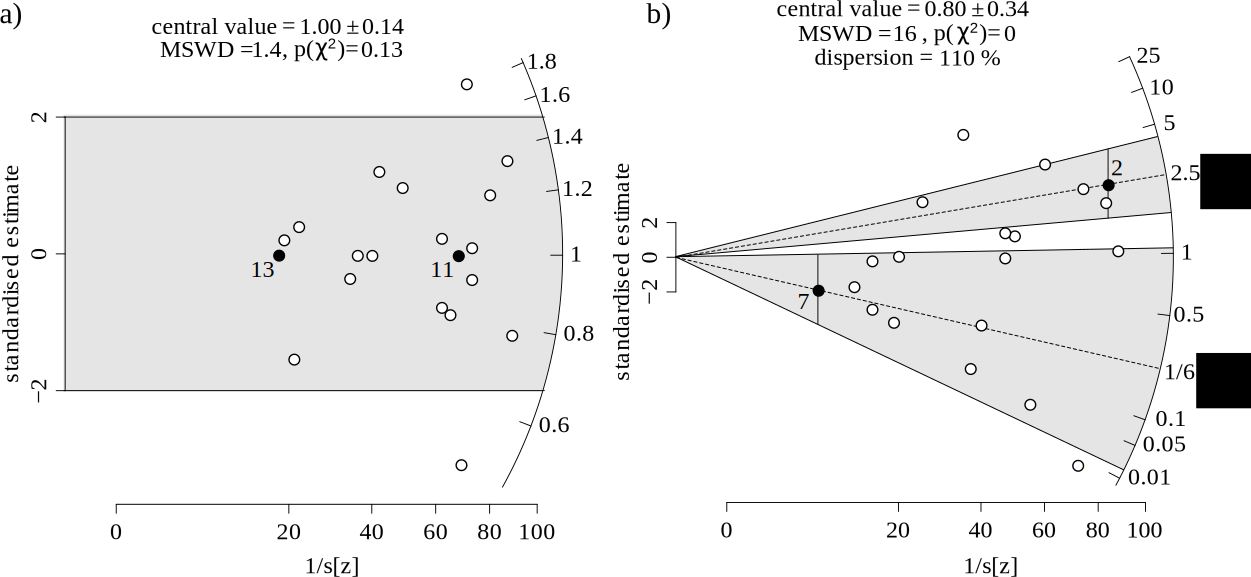
\includegraphics[width=.9\textwidth]{../figures/radial.pdf}
\end{center}
\begingroup \captionof{figure}{Radial plots for two synthetic datasets
  from \citet{vermeesch2018d}.  a) approximately 95\% of the samples
  in the first dataset plot within a symmetric `2-sigma' band around
  the origin. These data are therefore compatible with a single
  homogeneous population, and pass the chi-square test.  b) the age of
  each aliquot can be obtained by projecting the corresponding scatter
  point onto the radial scale.  Projecting a `2-sigma' error bar onto
  the same scale yields the 95\% confidence intervals of $t_2 = 2.5
  +1.7/-1.0$ and $t_{7} = 0.17 +1.20/-0.16$. The second sample does
  not fit within a `2-sigma' band, and is more adequately described by
  a random effects model with two parameters: the central ratio and
  the dispersion.\\}
  \label{fig:radial}
\endgroup

Radial plots are widely used in fission track and luminescence dating
\citep{galbraith1990a, galbraith1999}, but are yet to find their way
into other branches of geochronology. \texttt{IsoplotR} generalises
this valuable tool to all types of geochronological data.  In addition
to being an effective way to visualise heteroscedastic data, the
radial plot also represents a convenient vehicle for further data
interpretation and modelling, as will be discussed
Section~\ref{sec:mixtures}.\\

\noindent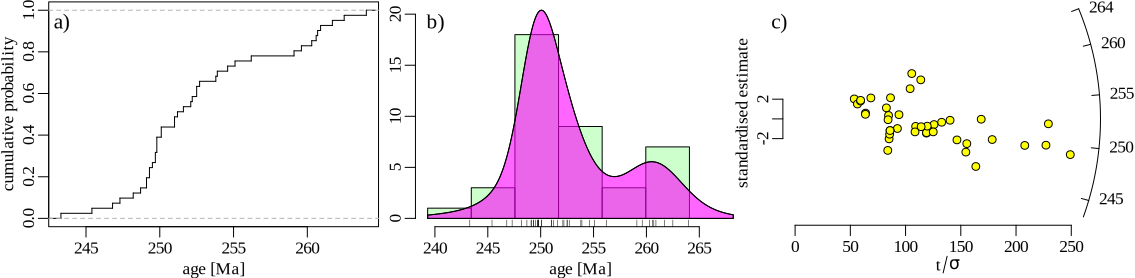
\includegraphics[width=\textwidth]{../figures/frequency.pdf}
\begingroup \captionof{figure}{a) CAD, b) histogram/KDE and c) radial
  plot of the same dataset \citep[from][]{ludwig2003}. }
\label{fig:density}
\endgroup

\section{Mixture models}
\label{sec:mixtures}

The weighted mean algorithm outlined in Sections~\ref{sec:mswd} and
\ref{sec:weightedmean} assumes that geochronological data obey normal
statistics. This assumption may be approximately correct for high
precision datasets but must inevitably be incorrect for low precision
ones.\\

Geologic time is a strictly positive quantity that is incompatible
with the symmetric Gaussian bell curve, which is defined over the
range of values from $-\infty$ to $+\infty$. Because geochronological
datasets must be strictly positive, their uncertainty distributions
must be asymmetric, with skewness being inversely proportional to
precision. This asymmetry is removed by the logarithmic transformation
that is used to construct radial plots
(Equation~\ref{eq:logtransform}), and which can also be applied to
KDEs:\\

\noindent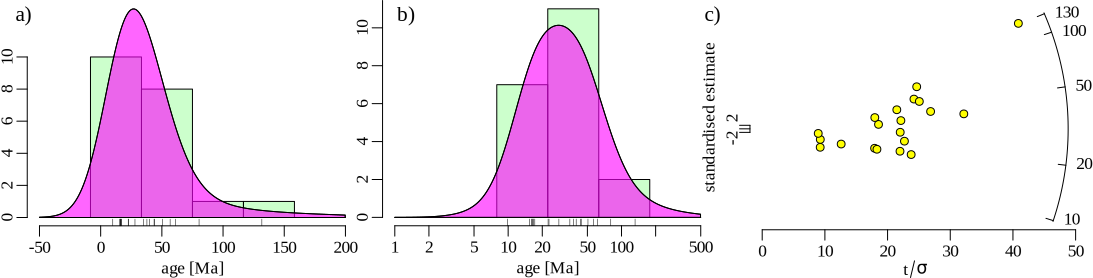
\includegraphics[width=\textwidth]{../figures/logtrans.pdf}
\begingroup
\captionof{figure}{Young U--Pb carbonate dates shown a) on a linear
  scale, whose KDE spills over into nonsensical negative data space,
  and b) on a logarithmic scale, which fixes this problem. c) shows
  the same data as a radial plot with a logarithmic time scale.\\}
\endgroup

We can reformulate Equation~\ref{eq:wtdmean} in terms of the
transformed variables $z_i$:
\begin{equation}
  p(z_i|\mu,\omega) = \mathcal{N}\left( \mu, \sigma^2 =
  s[z_i]^2+\omega^2 \right)
  \label{eq:central}
\end{equation}

\noindent which can be solved by the method of maximum likelihood as
before, yielding two estimates $\hat{\mu}$ and $\hat{\omega}$. The
\textbf{central age} is defined as $\exp(\hat{\mu})$, and
$\hat{\omega}$ represents the (over)dispersion of the data.  This is a
relative quantity (due to the log-transform) that estimates the
coefficient of variation of the true ages. The difference between the
central age and the weighted mean age is usually small unless the data
are imprecise and/or strongly overdispersed. In those cases, the
central age yields the geologically most meaningful value.\\

\noindent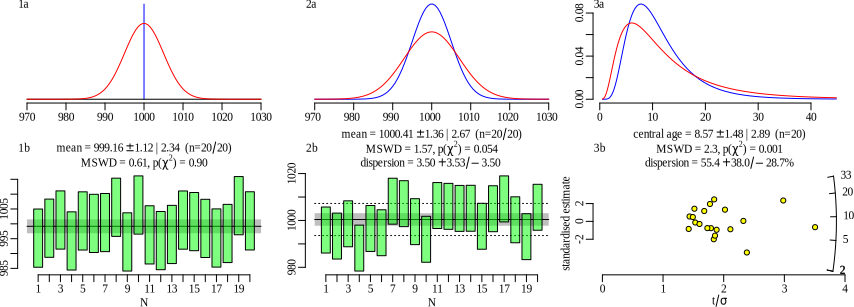
\includegraphics[width=\textwidth]{../figures/3means.pdf}
\begingroup \captionof{figure}{Three different age models implemented
  in \texttt{IsoplotR}. 1a) If the true age is a discrete event (blue
  peak at 1000~Ma), and the analytical uncertainties follow a normal
  distribution with zero mean and 5~Ma standard deviation, then the
  predicted distribution of the dates (red line) is a normal
  distribution with mean at 1000~Ma and a 5~Ma standard deviation. 1b)
  In this case the ordinary weighted mean (Equation~\ref{eq:wtdmean})
  is the most appropriate estimator of the true age. 2a) If the true
  age is drawn from a normal distribution with a mean of 1000~Ma and a
  standard deviation of 5~Ma (blue line), and if the analytical
  uncertainties follow a normal distribution with zero mean and 5~Ma
  standard deviation, then the predicted distribution of the dates
  (red line) is a normal distribution with mean at 1000~Ma and a
  $\sqrt{50}$~Ma standard deviation. 2b) In this case the random
  effects model of Equation~\ref{eq:wtdmean-model-3} is the most
  appropriate estimator of the mean \emph{and} the standard deviation
  of the true ages. The latter parameter is reported as the dispersion
  in the legend. 3a) If the true ages are drawn from a lognormal
  distribution with location parameter 10~Ma and a dispersion
  parameter of 50\% (blue line), and the analytical uncertainties are
  $\sim$50\%, then the distribution of the measured dates (red line)
  is a lognormal distribution with $10/\sqrt{2}$\% dispersion
  parameter. 3b) In this case the random effects model of
  Equation~\ref{eq:central} is the best way to average the data, and
  the radial plot with logarithmic scale is the best way to visualise
  the results.\\} \endgroup

The random effects model represented by Equation~\ref{eq:central} is
referred to as a \textbf{continuous mixture} model. It assumes that
the overdispersion of the data is caused by a continuous process that
yields a (log)normal distribution of true ages. As previously
mentioned in Section~\ref{sec:overdispersion}, one example of such a
process is the fractional crystallisation of plutons, which may take
hundreds of thousands of years, resulting in a range of zircon U-Pb
ages. A second example is the gradual cooling of tectonic blocks
during exhumation, which may cause the fission track system in
compositionally heterogeneous apatite populations to `close' at
different times. However, such continuous processes are by no means
the only cause of overdispersion in geochronology.\\

Consider, for instance, a detrital mixture originating from two or
more differently aged sources. Such a \textbf{discrete mixture} is
more adequately described by the following equation:
\begin{equation}
  \mathcal{LL}({\boldsymbol\mu},{\boldsymbol\pi}|\mathbf{z},\mathbf{s[z]}) =
  \sum_{i=1}^n\ln\!\left[\sum_{j=1}^k \pi_j \mathcal{N}\left( z_i | \mu_j, s[z_i]^2\right)\right]
  \label{eq:mixture}
\end{equation}

\noindent where ${\boldsymbol\mu}=\{\mu_1,\ldots,\mu_k\}$,
${\boldsymbol\pi}=\{\pi_1,\ldots,\pi_k\}$,
$\mathbf{z}=\{z_1,\ldots,z_k\}$,
$\mathbf{s[z]}=\{s[z_1],\ldots,s[z_k]\}$, $k$ is the number of
components, $\mu_j$ is the mean of the $j$\textsuperscript{th}
component (so that $\exp[\mu_j]$ is the corresponding age), and
$\pi_j$ is the proportion of the population that belongs to the
$j$\textsuperscript{th} component. Equation~\ref{eq:mixture} comprises
$n$ measurements and $2k-1$ unknowns ($\mu_j$ and $\pi_j$ for $1 \leq
j \leq k$ with $\pi_k=1-\sum_{j=1}^{k-1}\pi_j$). It can be solved by
the method of maximum likelihood.\\

\noindent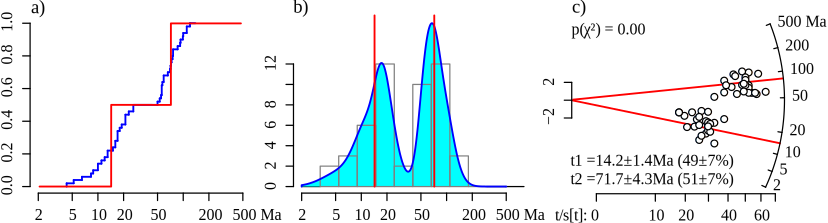
\includegraphics[width=\textwidth]{../figures/discretemixtures.pdf}
\begingroup \captionof{figure}{a) cumulative distribution of the true
  ages of a binary mixture of two discrete age components (red) and
  the CAD of the measured ages of 50 measured dates (blue). b)
  histogram and KDE of the binary mixture. c) results of the mixture
  model, shown as a radial plot.\\}
\label{fig:discretemixtures}
\endgroup

Choosing the right number of components ($k$) is a problem that merits
further discussion. \texttt{IsoplotR} implements the Bayes Information
Criterion (BIC) as a way to automatically pick the `optimal' value of
$k$ for any given dataset \citep[Section~5.6 of][]{galbraith2005}. But
this option should be used with caution because, for real datasets,
the number of components always increases with sample size. This
happens because the power of Equation~\ref{eq:mixture} to resolve even
the smallest degree of overdispersion increases with sample size.\\

Suppose that one uses the youngest component produced by the BIC
algorithm to estimate the maximum depositional age of a sedimentary
sequence. Then the resulting value would never converge to a specific
value.  Instead, one would find this minimum age to drift to ever
younger values until a point where the youngest age component in a
large dataset becomes younger than the actual depositional age. In
most cases it is, therefore, best to resist the temptation to use the
automatic peak fitting option. It is better to choose a specific
number of components instead, based on geological considerations.\\

\noindent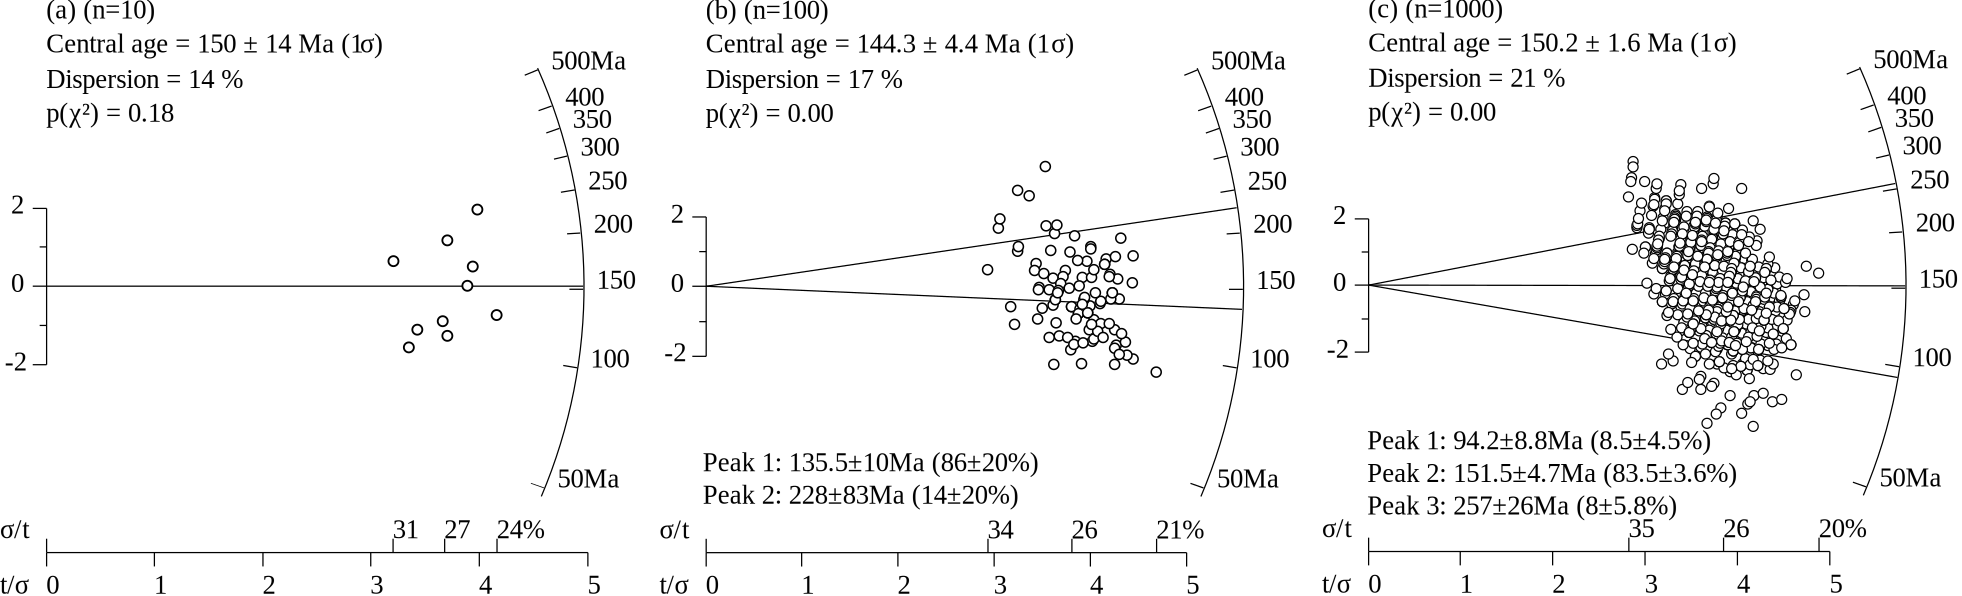
\includegraphics[width=\textwidth]{../figures/increasingn.pdf}
\begingroup \captionof{figure}{Application of finite mixture modelling
  to a continuous mixture. Increasing sample size from left (a) to
  right (c) provides statistical justification to fit more
  components. Note that the age of the youngest age component gets
  progressively younger with increasing sample size, from 150~Ma for
  sample (a) to 94~Ma for sample (c), and is therefore not a reliable
  estimator of the minimum age. Figure adapted from
  \citet{vermeesch2019b}.\\}
\label{fig:increasingn}
\endgroup

If one is mainly interested in the youngest age component, then it is
more productive to use an alternative parameterisation, in which all
grains are assumed to come from one of two components, whereby the
first component is a single discrete age peak ($\exp[\gamma]$, say)
and the second component ($\mathcal{N}'(\ldots)$) is a continuous
distribution such as Equation~\ref{eq:central}, but truncated at this
discrete value.
\begin{equation}
  \mathcal{LL}(\pi,\gamma,\mu,\omega|\mathbf{z},\mathbf{s[z]}) =
  \sum\limits_{j=1}^{n} \ln\!\left[
    \pi \mathcal{N}(z_i|\gamma,s[z_i]^2) +
    (1-\pi) \mathcal{N}'(z_i|\mu,s[z_i]^2+\omega^2)
    \right]
\label{eq:Lminagemod}
\end{equation}

One caveat is that, if this minimum age model is applied to relatively
small and/or high precision datasets such as most U-Pb measurements,
then the minimum age estimate will simply be equal to the youngest
date.  It is only for large and/or low precision datasets (such as
fission tracks), that the minimum age estimate will be older than then
youngest grain.  Crucially, this value will not drift to smaller
values with increasing sample size, but will converge to a distinct
minimum age.\\

\noindent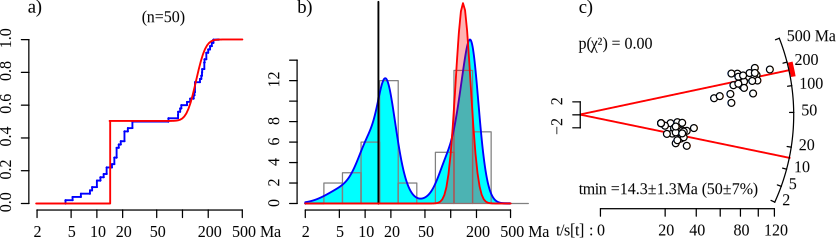
\includegraphics[width=\textwidth]{../figures/minagemod.pdf}
\begingroup \captionof{figure}{A binary mixture combining discrete and
  continuous age components shown as a) CADs and b) histograms and
  KDEs, with the true age components shown in red, and the measured
  age distribution in blue. c) radial plot with the minimum age model
  of Equation~\ref{eq:Lminagemod}.}
\label{fig:minagemod}
\endgroup

\printbibliography[heading=subbibliography]

\end{refsection}


\begin{refsection}

\chapter{U--Pb geochronology}\label{ch:U-Pb}

\section{Input formats}
\label{sec:UPbFormats}

\texttt{IsoplotR} offers eight different input formats:
\begin{enumerate}
  \item
  $\frac{07}{35}$,  
  $\mbox{err}\!\left[\frac{07}{35}\right]$, 
  $\frac{06}{38}$,  
  $\mbox{err}\!\left[\frac{06}{38}\right]$,  
  $\mbox{r}\!\left[\frac{06}{38},\frac{06}{38}\right]$
  \item $\frac{38}{06}$,  
  $\mbox{err}\!\left[\frac{38}{06}\right]$, 
  $\frac{07}{06}$,  
  $\mbox{err}\!\left[\frac{07}{06}\right]$,  
  $\left(\mbox{r}\!\left[\frac{38}{06},\frac{07}{06}\right]\right)$
  \item
  $\frac{07}{35}$,  
  $\mbox{err}\!\left[\frac{07}{35}\right]$, 
  $\frac{06}{38}$,  
  $\mbox{err}\!\left[\frac{06}{38}\right]$, 
  $\frac{07}{06}$,  
  $\mbox{err}\!\left[\frac{07}{06}\right]$, 
  $\left(\mbox{r}\!\left[\frac{07}{35},\frac{06}{38}\right]\right)$,  
  $\left(\mbox{r}\!\left[\frac{07}{35},\frac{07}{06}\right]\right)$, 
  $\left(\mbox{r}\!\left[\frac{06}{38},\frac{07}{06}\right]\right)$
  \item 
  $\frac{07}{35}$,  
  $\mbox{err}\!\left[\frac{07}{35}\right]$, 
  $\frac{06}{38}$,  
  $\mbox{err}\!\left[\frac{06}{38}\right]$,  
  $\frac{04}{38}$,  
  $\mbox{err}\!\left[\frac{04}{38}\right]$, 
  $\left(\mbox{r}\!\left[\frac{07}{35},\frac{06}{38}\right]\right)$,  
  $\left(\mbox{r}\!\left[\frac{07}{35},\frac{04}{38}\right]\right)$, 
  $\left(\mbox{r}\!\left[\frac{06}{38},\frac{04}{38}\right]\right)$
  \item 
  $\frac{38}{06}$,  
  $\mbox{err}\!\left[\frac{38}{06}\right]$, 
  $\frac{07}{06}$,  
  $\mbox{err}\!\left[\frac{07}{06}\right]$,  
  $\frac{04}{06}$,  
  $\mbox{err}\!\left[\frac{04}{06}\right]$, 
  $\left(\mbox{r}\!\left[\frac{38}{06},\frac{07}{06}\right]\right)$,  
  $\left(\mbox{r}\!\left[\frac{38}{06},\frac{04}{06}\right]\right)$, 
  $\left(\mbox{r}\!\left[\frac{07}{06},\frac{04}{06}\right]\right)$
  \item 
  $\frac{07}{35}$,  
  $\mbox{err}\!\left[\frac{07}{35}\right]$, 
  $\frac{06}{38}$,  
  $\mbox{err}\!\left[\frac{06}{38}\right]$,  
  $\frac{04}{38}$,  
  $\mbox{err}\!\left[\frac{04}{38}\right]$,  
  $\frac{07}{06}$,  
  $\mbox{err}\!\left[\frac{07}{06}\right]$, 
  $\frac{04}{07}$,  
  $\mbox{err}\!\left[\frac{04}{07}\right]$,  
  $\frac{04}{06}$,  
  $\mbox{err}\!\left[\frac{04}{06}\right]$
  \item 
  $\frac{07}{35}$,  
  $\mbox{err}\!\left[\frac{07}{35}\right]$, 
  $\frac{06}{38}$,  
  $\mbox{err}\!\left[\frac{06}{38}\right]$,  
  $\frac{08}{32}$,  
  $\mbox{err}\!\left[\frac{08}{32}\right]$,  
  $\frac{32}{38}$,  
  $\mbox{err}\!\left[\frac{32}{38}\right]$,  \\
  $\left(\mbox{r}\!\left[\frac{07}{35},\frac{06}{38}\right]\right)$,  
  $\left(\mbox{r}\!\left[\frac{07}{35},\frac{08}{32}\right]\right)$, 
  $\left(\mbox{r}\!\left[\frac{07}{35},\frac{32}{38}\right]\right)$,  
  $\left(\mbox{r}\!\left[\frac{06}{38},\frac{08}{32}\right]\right)$,  
  $\left(\mbox{r}\!\left[\frac{06}{38},\frac{32}{38}\right]\right)$, 
  $\left(\mbox{r}\!\left[\frac{08}{32},\frac{32}{38}\right]\right)$
  \item
  $\frac{38}{06}$,  
  $\mbox{err}\!\left[\frac{38}{06}\right]$, 
  $\frac{07}{06}$,  
  $\mbox{err}\!\left[\frac{07}{06}\right]$,  
  $\frac{08}{06}$,  
  $\mbox{err}\!\left[\frac{08}{06}\right]$,  
  $\frac{32}{38}$,  
  $\mbox{err}\!\left[\frac{32}{38}\right]$,  \\
  $\left(\mbox{r}\!\left[\frac{38}{06},\frac{07}{06}\right]\right)$,  
  $\left(\mbox{r}\!\left[\frac{38}{06},\frac{08}{06}\right]\right)$, 
  $\left(\mbox{r}\!\left[\frac{38}{06},\frac{32}{38}\right]\right)$,  
  $\left(\mbox{r}\!\left[\frac{07}{06},\frac{08}{06}\right]\right)$,  
  $\left(\mbox{r}\!\left[\frac{07}{06},\frac{32}{38}\right]\right)$, 
  $\left(\mbox{r}\!\left[\frac{08}{06},\frac{32}{38}\right]\right)$
\end{enumerate}

\noindent where 04, 06, 07, 08, 32, 35 and 38 stand for
\textsuperscript{204}Pb, \textsuperscript{206}Pb,
\textsuperscript{207}Pb, \textsuperscript{208}Pb,
\textsuperscript{232}Th, \textsuperscript{235}U and
\textsuperscript{238}U, respectively. `err[$\ast$]' stands for the
analytical uncertainty of $\ast$, which can be specified as a standard
error or as two times the standard error, either in absolute or
relative units. And `r[$x$,$y$]' stands for the error correlation
between $x$ and $y$.\\

Formats~1--3 are meant for mass spectrometers that are unable to
accurately measure \textsuperscript{204}Pb. This is the case for
single collector ICP-MS instruments that are unable to resolve the
isobaric interference on \textsuperscript{204}Hg, which is often
present in the plasma gas. Formats~4--6 include
\textsuperscript{204}Pb, as measured by SIMS, TIMS or multi-collector
ICP-MS. Finally, formats~7 and 8 include \textsuperscript{208}Pb and
\textsuperscript{232}Th. These nuclides can be used for hybrid
U--Th--Pb dating, as discussed in Section~\ref{sec:U-Th-Pb}.\\

Formats~1, 4 and 7 are `Wetherill style' input formats, in which the
radioactive parent appears in the denominator of the isotopic ratio
data. As explained in Section~\ref{sec:errorcorrelations} and shown in
Figure~\ref{fig:errorcorrelation}, these formats are associated with
strong error correlations
($r\left[\frac{07}{35},\frac{06}{38}\right]$), which must be specified
so as to avoid inaccurate inferences.  Formats~2, 5 and 8 are
`Tera-Wasserburg style' input formats, in which the most abundant
radiogenic daughter (i.e., \textsuperscript{206}Pb) appears in the
denominator of the isotopic ratio data.  As shown in
Figure~\ref{fig:inverrorcorrelation}, this greatly reduces the error
correlations which, consequently, are optional (hence the brackets
around $r\left[\frac{38}{06},\frac{07}{06}\right]$).\\

Finally, formats~3 and 6 provide an alternative input format designed
for users whose low level data processing software does not provide
error correlation data. It uses redundant ratios to infer the
correlation coefficients. Let $X \equiv \frac{07}{35}$, $Y \equiv
\frac{07}{35}$, $Z \equiv \frac{07}{06}$ and $U \equiv \frac{38}{35}$,
let $s[X]$, $s[Y]$ and $s[Z]$ be the standard errors of $X$, $Y$ and
$Z$, and assume that $s[U]=0$ for the sake of simplicity. Then it is
easy to see that $Z = X/(U Y)$, and
\begin{equation}
  \left(\frac{s[Z]}{Z}\right)^2 = \left(\frac{s[X/Y]}{X/Y}\right)^2
  \approx \left(\frac{s[X]}{X}\right)^2 + \left(\frac{s[Y]}{Y}\right)^2 -
  2 \frac{s[X,Y]}{XY}
\end{equation}

\noindent from which the covariance (and, hence, the correlation
coefficient) between $X$ and $Y$ can be inferred as
\begin{equation}
  s[X,Y] \approx \frac{XY}{2}
  \left[
    \left(\frac{s[X]}{X}\right)^2 +
    \left(\frac{s[Y]}{Y}\right)^2 -
    \left(\frac{s[Z]}{Z}\right)^2
    \right]
\end{equation}

It is important to note that this approach makes the crucial
assumption that all three standard errors ($s[X]$, $s[Y]$ and $s[Z]$)
are based on the same number of data points. This means that formats~3
and 6 are not applicable to TIMS data.

\section{Concordia diagrams and ages}
\label{sec:concordia}

\texttt{IsoplotR} implements three types of concordia diagram:

\begin{enumerate}
\item The \textbf{Wetherill} concordia diagram sets out the
  \textsuperscript{206}Pb/\textsuperscript{238}U vs. the
  \textsuperscript{207}Pb/\textsuperscript{235}U ratios. This format
  introduces relatively strong error correlations (see
  Section~\ref{sec:errorcorrelations}). The addition of common Pb
  pulls samples away from concordia along a line whose slope is
  proportional to the common Pb composition. Isotopic compositions
  above the concordia line are `forbidden'. They could, in principle,
  be caused by U-loss. But in practice this mechanism is implausible.
\item The \textbf{Tera-Wasserburg} concordia diagram uses the inverse
  isochron ratios \textsuperscript{207}Pb/\textsuperscript{206}Pb vs.
  and \textsuperscript{238}U/\textsuperscript{206}Pb. This format
  exhibits weaker error correlations. The addition of common Pb
  creates a binary mixing line between radiogenic and common Pb
  compositions (see Section~\ref{sec:discordia}). The area below the
  concordia line is `forbidden' and the only reason why samples may
  plot there is due to random chance and analytical imprecision.
\item The \textbf{U--Th--Pb concordia} diagram sets out the
  conventional isochron ratios of
  \textsuperscript{208}Pb/\textsuperscript{232}Th vs.
  \textsuperscript{206}Pb/\textsuperscript{238}U. Like the Wetherill
  diagram, the U--Th--Pb diagram also exhibits strong error
  correlations.  But in contrast with the Wetherill diagram, the
  addition of common Pb does not necessarily create linear trends on
  the U--Th--Pb diagram. Instead, different aliquots may end up on
  either side of the concordia line depending on their Th/U ratio.
\end{enumerate}

The Wetherill and Tera-Wasserburg concordia plots are available to
datasets from any of \texttt{IsoplotR}'s eight input formats,
irrespective of whether the ratios are stored in a Wetherill or
Tera-Wasserburg format. \texttt{IsoplotR} automatically handles the
data conversions internally. The U--Th--Pb concordia plot is only
available for data formats~7 and 8, because these are the only formats
that account for \textsuperscript{208}Pb and \textsuperscript{232}Th.
The remainder of this Chapter will focus on the Wetherill and
Tera-Wasserburg diagrams, except for Section~\ref{sec:common-Pb},
which will briefly mention the U--Th-Pb diagram again.

\noindent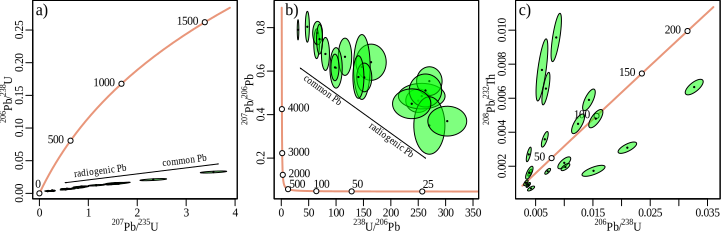
\includegraphics[width=\textwidth]{../figures/3xconcordia.pdf}
\begingroup \captionof{figure}{The allanite dataset of
  \citet{janots2014} shown on a) Wetherill, b) Tera-Wasserburg and c)
  U--Th--Pb concordia diagram.}\endgroup

In the absence of (or after correction for) common Pb or other
complications, multiple aliquots from the same sample may plot on the
concordia line. Such samples are said to be concordant. Their `most
likely' age (in a statistical sense) is known as the \textbf{concordia
  age}. Calculating a concordia age involves two steps
\citep{ludwig1998}:

\begin{enumerate}
  \item Calculate the two-dimensional error-weighted average
    ($\{\bar{x},\bar{y}\}$) of the U--Pb ratios, by maximising the
    likelihood function. In Wetherill space:
    \[
    \mathcal{LL} \propto
    - \sum\limits_{i=1}^{n}
    \left[
      \begin{array}{@{}c@{}}
        \left[\frac{07}{35}\right]_i-\bar{x}\\
        \left[\frac{06}{38}\right]_i-\bar{y}
      \end{array}
      \right]^T
    \left[
      \begin{array}{@{}cc@{}}
        s\!\left[\frac{07}{35}\right]_i^2 &
        s\!\left[\frac{07}{35},\frac{06}{38}\right]_i\\
        s\!\left[\frac{07}{35},\frac{06}{38}\right]_i &
        s\!\left[\frac{06}{38}\right]_i^2
      \end{array}
      \right]^{-1}
    \left[
      \begin{array}{@{}c@{}}
        \left[\frac{07}{35}\right]_i-\bar{x}\\
        \left[\frac{06}{38}\right]_i-\bar{y}
      \end{array}
      \right]    
    \]

    or in Tera-Wasserburg space:
        \[
    \mathcal{LL} \propto
    - \sum\limits_{i=1}^{n}
    \left[
      \begin{array}{@{}c@{}}
        \left[\frac{38}{06}\right]_i-\bar{x}\\
        \left[\frac{07}{06}\right]_i-\bar{y}
      \end{array}
      \right]^T
    \left[
      \begin{array}{@{}cc@{}}
        s\!\left[\frac{38}{06}\right]_i^2 &
        s\!\left[\frac{38}{06},\frac{07}{06}\right]_i\\
        s\!\left[\frac{38}{06},\frac{07}{06}\right]_i &
        s\!\left[\frac{07}{06}\right]_i^2
      \end{array}
      \right]^{-1}
    \left[
      \begin{array}{@{}c@{}}
        \left[\frac{38}{06}\right]_i-\bar{x}\\
        \left[\frac{07}{06}\right]_i-\bar{y}
      \end{array}
      \right]    
    \]

    Using standard maximum likelihood theory, the covariance matrix of
    the weighted mean composition ($\Sigma_{\bar{x},\bar{y}}$) is
    obtained by inverting the matrix of second derivatives of
    $\mathcal{LL}$.
    
  \item Given the concordia composition $\{\bar{x},\bar{y}\}$ obtained
    in the previous step, compute the most likely age ($t_c$) of this
    concordia composition. This is again done using the method of
    maximum likelihood. In Wetherill space:
        \[
    \mathcal{LL} \propto
    - \sum\limits_{i=1}^{n}
    \left[
      \begin{array}{@{}c@{}}
        \bar{x} - (\exp[\lambda_{235}t_c] - 1)\\
        \bar{y} - (\exp[\lambda_{238}t_c] - 1)
      \end{array}
      \right]^T
    \Sigma_{\bar{x},\bar{y}}^{-1}
    \left[
      \begin{array}{@{}c@{}}
        \bar{x} - (\exp[\lambda_{235}t_c] - 1)\\
        \bar{y} - (\exp[\lambda_{238}t_c] - 1)
      \end{array}
      \right]
    \]

    Or in Tera-Wasserburg space:
        \[
    \mathcal{LL} \propto
    - \sum\limits_{i=1}^{n}
    \left[
      \begin{array}{@{}c@{}}
        \bar{x} - \frac{1}{\exp[\lambda_{238}t_c] - 1}\\
        \bar{y} - \left[\frac{35}{38}\right]
        \frac{\exp[\lambda_{235}t_c] - 1}
             {\exp[\lambda_{238}t_c] - 1}
      \end{array}
      \right]^T
    \Sigma_{\bar{x},\bar{y}}^{-1}
    \left[
      \begin{array}{@{}c@{}}
        \bar{x} - \frac{1}{\exp[\lambda_{238}t_c] - 1}\\
        \bar{y} - \left[\frac{35}{38}\right]
        \frac{\exp[\lambda_{235}t_c] - 1}
             {\exp[\lambda_{238}t_c] - 1}
      \end{array}
      \right]^T
    \]

    Again, the uncertainty of $t_c$ is obtained by inverting the
    Fisher information matrix.
    
\end{enumerate}

\noindent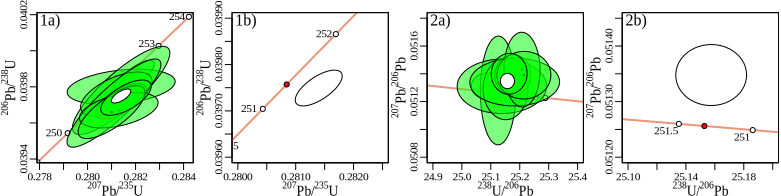
\includegraphics[width=\textwidth]{../figures/concordia_age.pdf}
\begingroup \captionof{figure}{1) Wetherill and 2) Tera-Wasserburg
  concordia diagram with a) the weighted mean composition shown as
  white error ellipse, and b) the maximum concordia age shown as a red
  circle.}\endgroup


\printbibliography[heading=subbibliography]

\end{refsection}


\chapter{Pb--Pb and Th--Pb}\label{ch:Th-Pb-Pb}


\begin{refsection}

\chapter{Ar--Ar and K--Ca}\label{ch:ArArKCa}

The Ar--Ar and K--Ca chronometers are based on the branched decay of
\textsuperscript{40}K to \textsuperscript{40}Ar and
\textsuperscript{40}Ca. The Ar--Ar is a widely used method that has
replaced the K--Ar method in all but a few applications
(Section~\ref{sec:K-Ar}). The K--Ca method is a less common method
that is becoming more feasible due to analytical advances in SIMS,
which have resolved the isobaric interference between
\textsuperscript{40}K and \textsuperscript{40}Ca
\citep{harrison2010}. The original K--Ar method is not implemented in
\texttt{IsoplotR} but may be added later.

\section{Ar--Ar}\label{sec:ArAr}

\texttt{IsoplotR} offers three input formats for Ar--Ar data, which
all require the user to provide the J factor and its standard error
(Section~\ref{sec:Ar-Ar}), as well as the following columns of
isotopic ratio data:
\begin{enumerate}
\item{`Normal':}
  $\frac{40}{36}$,  
  $\mbox{err}\!\left[\frac{40}{36}\right]$, 
  $\frac{39}{36}$,  
  $\mbox{err}\!\left[\frac{39}{36}\right]$,  
  $\mbox{r}\!\left[\frac{40}{36},\frac{39}{36}\right]$,
  $\left(39\right)$
\item{`Inverse':}
  $\frac{39}{40}$,  
  $\mbox{err}\!\left[\frac{39}{40}\right]$, 
  $\frac{36}{40}$,  
  $\mbox{err}\!\left[\frac{36}{40}\right]$,  
  $\left(\mbox{r}\!\left[\frac{39}{40},\frac{36}{40}\right]\right)$,
  $\left(39\right)$
\item{`Three ratios':}
  $\frac{39}{40}$,  
  $\mbox{err}\!\left[\frac{39}{40}\right]$, 
  $\frac{36}{40}$,  
  $\mbox{err}\!\left[\frac{36}{40}\right]$,  
  $\frac{39}{36}$,  
  $\mbox{err}\!\left[\frac{39}{36}\right]$,
  $\left(39\right)$
\end{enumerate}

\noindent where $(39)$ stands for the amount of \textsuperscript{39}Ar
in each heating step, which is normalised by \texttt{IsoplotR} to form
the X-axis of an age spectrum (Section~\ref{sec:agespectra}). Error
correlations are much stronger for format~1 than for format~2 and are
therefore compulsory for the former and optional for the latter. Just
like the Pb--Pb and Th--Pb methods, the names of the formats refer to
the normal and inverse isochrons that they form. Despite this
nomenclature, both normal and inverse isochrons are available for all
three methods, with \texttt{IsoplotR} converting them in the
background using Equation~\ref{eq:redundantratios} for the conversion
from format~3 to format~2; and using
Equation~\ref{eq:format12transformation} to convert format~2 to
format~1 and vice versa.

In complete analogy with Figure~\ref{fig:ThPbSingleGrain}, single
grain ages can be calculated by projecting cogenetic aliquots along an
isochron, or by applying a nominal `excess argon' correction to each
aliquot separately. The latter approach typically uses the atmospheric
argon composition, which is characterised by a
\textsuperscript{40}Ar/\textsuperscript{39}Ar ratio of
$298.56\pm{0.31}$ \citep{lee2006}. The resulting ages can then be
visualised as radial plots, KDEs, or CADs:\\

\noindent\begin{minipage}[t][][b]{.7\linewidth}
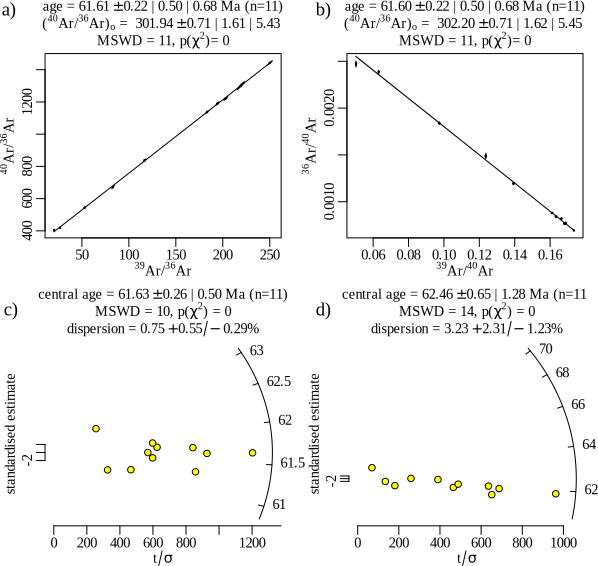
\includegraphics[width=\textwidth]{../figures/ArAr.pdf}
\end{minipage}
\begin{minipage}[t][][t]{.3\linewidth}
  \captionof{figure}{a) conventional and b) inverse model-1 isochron
    for Ar--Ar data. The non-radiogenic (`excess') argon is
    characterised by a \textsuperscript{40}Ar/\textsuperscript{39}Ar
    ratio of 302, which is slightly higher than atmosphere.  c) shows
    a radial plot of the excess-Ar-corrected ages obtained by
    projecting the aliquots along the inverse isochron (just like in
    Figure~\ref{fig:ThPbSingleGrain}.a). d) using the atmospheric
    ratio of $298.56\pm{0.31}$ to correct each aliquot independently
    yields a slightly older and more dispersed distribution.}
  \label{fig:radialArArisochron}
\end{minipage}

\section{Age spectra}\label{sec:agespectra}

As explained in Section~\ref{sec:Ar-Ar}, the
\textsuperscript{40}Ar/\textsuperscript{39}Ar-age spectrum is a useful
tool to visualise stepwise heating measurements. Its appearance is
based on the weighted mean plot (e.g., Figure~\ref{fig:wtdmeanMSWD}),
with the different heating steps arranged in order of increasing
degree of degassing along the horizontal axis, and the width of the
different sample boxes proportional to the corresponding amounts of
\textsuperscript{39}Ar.\\

\texttt{IsoplotR} defines the `plateau age' as the weighted mean age
of the longest sequence (in terms of cumulative \textsuperscript{39}Ar
content) of consecutive heating steps that pass the modified Chauvenet
criterion of Section~\ref{ch:generic}. Note that this definition is
different (and simpler) than the one used by \texttt{Isoplot}
\citep{ludwig2003}. However, it is important to mention that all
definitions of an age plateau are heuristic by nature and should not
be used for quantitative inference.

\begin{center}
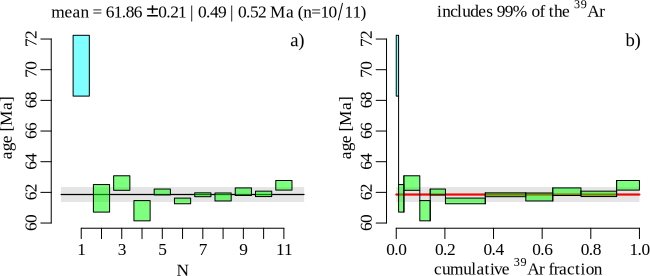
\includegraphics[width=.85\textwidth]{../figures/agespectrum.pdf}
\captionsetup{width=.85\textwidth}
\captionof{figure}{a) weighted mean and b) age spectrum for the Ar--Ar
  of Figure~\ref{fig:radialArArisochron}, using an atmospheric
  \textsuperscript{40}Ar/\textsuperscript{39}Ar-ratio for the
  non-radiogenic component.  The plateau is shown in green and the
  single outlier in blue. The weighted mean age was calculated using
  an ordinary weighted mean. In this case the weighted mean age and
  the plateau age are the same but this is not always the case.}
\label{fig:agespectrum}
\end{center}

\section{K--Ca}\label{sec:K-Ca}

\texttt{IsoplotR} offers three input formats for K--Ca data:
\begin{enumerate}
\item{`Normal':}
  $\frac{{}^{40}\mbox{K}}{{}^{44}\mbox{Ca}}$,  
  $\mbox{err}\!\left[\frac{{}^{40}\mbox{K}}{{}^{44}\mbox{Ca}}\right]$, 
  $\frac{{}^{40}\mbox{Ca}}{{}^{44}\mbox{Ca}}$,
  $\mbox{err}\!\left[\frac{{}^{40}\mbox{Ca}}{{}^{44}\mbox{Ca}}\right]$,  
  $\mbox{r}\!\left[\frac{{}^{40}\mbox{K}}{{}^{44}\mbox{Ca}},
    \frac{{}^{40}\mbox{Ca}}{{}^{44}\mbox{Ca}}\right]$
\item{`Inverse':}
  $\frac{{}^{40}\mbox{K}}{{}^{40}\mbox{Ca}}$,  
  $\mbox{err}\!\left[\frac{{}^{40}\mbox{K}}{{}^{40}\mbox{Ca}}\right]$, 
  $\frac{{}^{44}\mbox{Ca}}{{}^{40}\mbox{Ca}}$,  
  $\mbox{err}\!\left[\frac{{}^{44}\mbox{Ca}}{{}^{40}\mbox{Ca}}\right]$,  
  $\mbox{r}\!\left[\frac{{}^{40}\mbox{K}}{{}^{40}\mbox{Ca}},
    \frac{{}^{44}\mbox{Ca}}{{}^{40}\mbox{Ca}}\right]$
\item{`Three ratios':}
  $\frac{{}^{40}\mbox{K}}{{}^{44}\mbox{Ca}}$,  
  $\mbox{err}\!\left[\frac{{}^{40}\mbox{K}}{{}^{44}\mbox{Ca}}\right]$, 
  $\frac{{}^{40}\mbox{Ca}}{{}^{44}\mbox{Ca}}$,
  $\mbox{err}\!\left[\frac{{}^{40}\mbox{Ca}}{{}^{44}\mbox{Ca}}\right]$,  
  $\frac{{}^{40}\mbox{K}}{{}^{40}\mbox{Ca}}$,  
  $\mbox{err}\!\left[\frac{{}^{40}\mbox{K}}{{}^{40}\mbox{Ca}}\right]$
\end{enumerate}

\noindent where, in contrast with previous formatting summaries, the
full names of the nuclides are given because of the isobaric parent
and daughter. It is precisely this isobary that prevented the K--Ca
from being applicable by in-situ methods until recently. Formats~1, 2
and 3 can be converted to each other using
Equations~\ref{eq:redundantratios} and
\ref{eq:format12transformation}.\\

\texttt{IsoplotR} uses \textsuperscript{44}Ca as a normalising isotope
because it is the most abundant of calcium's non-radiogenic isotopes,
accounting for up to 2\% of the isotopic budget. Using a less abundant
isotope such as \textsuperscript{42}Ca ($<0.647\%$),
\textsuperscript{43}Ca ($<0.135\%$), or \textsuperscript{46}Ca
($<0.004\%$), would only increase the error correlations in
conventional isochron space (which are already very strong as shown in
Figure~\ref{fig:errorcorrelation}). However, \texttt{IsoplotR} also
offers inverse isochrons, which greatly reduce these correlations as
explained in Section~\ref{sec:errorcorrelations} and shown in
Figure~\ref{fig:inverrorcorrelation}.

\printbibliography[heading=subbibliography]

\end{refsection}


\begin{refsection}

\chapter{Rb--Sr, Sm--Nd, Lu--Hf and Re--Os}\label{ch:PD}

Rb--Sr, Sm--Nd, Lu--Hf and Re--Os all fall in the category of simple
parent-daughter chronometers, which are based on a single parent that
decays to a single daughter without additional complications such as
branched decay or secular equilibrium. These chronometers usually
involve liquid chromatography and mass spectrometry by TIMS or
solution ICP-MS. Data can be introduced into \texttt{IsoplotR} in
three formats:

\begin{enumerate}
\item{`Normal':}
  $\frac{\mbox{P}}{\mbox{d}}$,  
  $\mbox{err}\!\left[\frac{\mbox{P}}{\mbox{d}}\right]$, 
  $\frac{\mbox{D}}{\mbox{d}}$,  
  $\mbox{err}\!\left[\frac{\mbox{D}}{\mbox{d}}\right]$,  
  $\mbox{r}\!\left[\frac{\mbox{P}}{\mbox{d}},
  \frac{\mbox{D}}{\mbox{d}}\right]$
\item{`Inverse':}
  $\frac{\mbox{P}}{\mbox{D}}$,  
  $\mbox{err}\!\left[\frac{\mbox{P}}{\mbox{D}}\right]$, 
  $\frac{\mbox{d}}{\mbox{D}}$,  
  $\mbox{err}\!\left[\frac{\mbox{d}}{\mbox{D}}\right]$,  
  $\mbox{r}\!\left[\frac{\mbox{P}}{\mbox{D}},
  \frac{\mbox{d}}{\mbox{D}}\right]$
\item{`Concentrations':}
  \textbf{P}, err[\textbf{P}], \textbf{D}, err[\textbf{D}], P/D
\end{enumerate}

\noindent where

\noindent P = \textsuperscript{87}Rb, \textsuperscript{147}Sm,
\textsuperscript{187}Re or \textsuperscript{176}Lu.

\noindent D = \textsuperscript{87}Sr, \textsuperscript{143}Nd,
\textsuperscript{187}Os or \textsuperscript{176}Hf.

\noindent d = \textsuperscript{86}Sr, \textsuperscript{144}Nd,
\textsuperscript{188}Os or \textsuperscript{177}Hf.

\noindent \textbf{P} = the elemental concentration (in ppm) of Rb, Sm,
Re, or Lu.

\noindent \textbf{D} = the elemental concentration (in ppm) of Sr, Nd,
Os, or Hf.\\

Format~1 can be converted to format~2 (and vice versa) using
Equation~\ref{eq:format12transformation}, whereas Format~3 can be
converted to format~1 with the methods that were used in
Chapter~\ref{ch:exercises}. For example, for Rb--Sr:
\begin{equation}
  \left({}^{87}\mbox{Rb}/{}^{86}\mbox{Sr}\right) = 
  \frac{\mbox{\textbf{Rb}}}{\mbox{\textbf{Sr}}}
  \frac{\mbox{M(Rb)}}{\mbox{M(Sr)}}
  \frac{
    1+\left[{{}^{87}\mbox{Sr}}/{{}^{86}\mbox{Sr}}\right]
    \left[1+({}^{84}\mbox{Sr}/{}^{87}\mbox{Sr}) +
      ({}^{88}\mbox{Sr}/{}^{87}\mbox{Sr}) \right]
  }{
    1+[{}^{85}\mbox{Rb}/{}^{87}\mbox{Rb}]
  }
  \label{eq:ppm2ratios}
\end{equation}

\noindent where (\textsuperscript{84}Sr/\textsuperscript{87}Sr),
(\textsuperscript{88}Sr/\textsuperscript{87}Sr) and
(\textsuperscript{85}Rb/\textsuperscript{87}Rb) are constant,
non-radiogenic isotope ratios, and M(Rb) and M(Sr) are the molar
masses of Rb and Sr, respectively. Because the measured
(\textsuperscript{87}Sr/\textsuperscript{86}Sr)-ratio appears in
Equation~\ref{eq:ppm2ratios}, the covariance between
\textsuperscript{87}Rb/\textsuperscript{86}Sr and
\textsuperscript{87}Sr/\textsuperscript{86}Sr is nonzero and can be
estimated using Equation~\ref{eq:s2t} or \ref{eq:s2tmatrix}.\\

The parent-daughter pair methods are generally used to form
multi-aliquot isochrons that can either be plotted in conventional or
inverse isochron space. For the U--Pb, Ar--Ar, Pb--Pb and K-Ca
methods, the nonradiogenic daughter isotope is less abundant than the
radiogenic isotope. However this is not the case for the Rb--Sr,
Sm--Nd, Re--Os and Lu--Hf methods. Their non-radiogenic isotopes
(marked as `d' above) tend to be more abundant than the radiogenic
isotope and they therefore exhibit weaker error correlations in
conventional isotope space. Nevertheless, \texttt{IsoplotR} does offer
the inverse isochron as an option because it is may still be useful to
visualise the data as a simple mixing line between non-radiogenic and
radiogenic components.\\

\noindent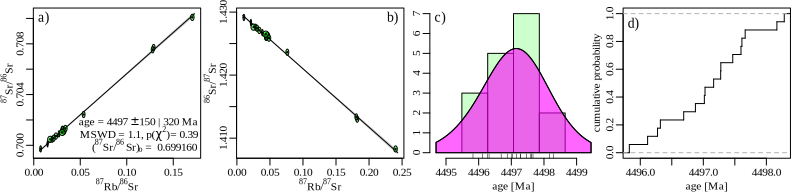
\includegraphics[width=\textwidth]{../figures/RbSr.pdf}
\begingroup\captionof{figure}{a) conventional and b) inverse Rb--Sr
  isochron, c) KDE and d) CAD of the single aliquot age estimates
  using the isochron intercept as a non-radiogenic
  \textsuperscript{87}Sr/\textsuperscript{86}Sr-ratio.\\}
\label{fig:RbSrabcd}\endgroup

The distribution of the data around the best fit isochron can be
visually assessed on radial plots, KDEs and CADs. This is achieved by
projecting the data along parallel lines to the best fit in inverse
isochron space as in
Figure~\ref{fig:ThPbSingleGrain}.a. Alternatively, the assumption of
cogenetic origin may be relaxed by fixing the non-radiogenic
composition and computing two-point isochrons between this composition
and the measured ratios for each aliquot
(Figure~\ref{fig:ThPbSingleGrain}.b).

\printbibliography[heading=subbibliography]

\end{refsection}


\begin{refsection}

\chapter{U--Th--(Sm)--He}\label{ch:UThHe}

\texttt{IsoplotR} offers a single input format for U--Th--(Sm)--He
data that can be captured by the following columns:

\begin{center}
He, err[He], U, err[U], Th, err[Th], Sm, err[Sm]
\end{center}

\noindent which contains all the necessary information to calculate
the age. Rewriting Equation~\ref{eq:U-Th-He}:
\begin{equation}
\begin{split}
  \left[^4\mbox{He}\right] = & ~a(t) 
   \mbox{[U]} + b(t)\mbox{[Th]} + c(t)\mbox{[Sm]} \\
   \mbox{where~} a(t) = &
   \left[8 \frac{137.818}{138.818} (e^{\lambda_{238}t} - 1) +
     7 \frac{1}{138.818} (e^{\lambda_{235}t} - 1) \right] \\
   b(t) = & ~6 (e^{\lambda_{232}t} - 1)\\
    \mbox{and~} c(t) = & ~0.1499 (e^{\lambda_{147}t} - 1)
\end{split}
\label{eq:UThHe2}
\end{equation}

Because Sm (1) produces only one \textalpha-particle per decay event;
(2) has a very long half-life; and (3) its radioactive isotope 147
only accounts for 14.99\% of total samarium, Sm can be ignored as a
parent in all but the most Sm-rich samples. For this reason, some
laboratories do not measure Sm at all, and the `Sm' and `err[Sm]'
columns are optional. If omitted, \texttt{IsoplotR} will simply assume
that the Sm-concentration is zero.\\

The He, U, Th (and Sm) measurements must be expressed in internally
consistent \textbf{atomic units} such as mol, fmol, pmol, mol/cc,
fmol/\textmu{g} etc. They must not be expressed in mass units such as
ppm, ppb or wt\%! For U and Sm, which are poly-isotopic elements, it
is the total amount that is required, and not just
\textsuperscript{238}U and \textsuperscript{147}Sm. A second important
requirement is that the data have been corrected for
\textbf{\textalpha-ejection} prior to analysis, as explained in the
next section.

\section{The \textalpha-ejection correction}\label{sec:alpha-ejection}

Helium, like argon, is a noble gas that is lost to the environment
(and eventually to space) at high temperatures by volume diffusion.
Additional complication is added by the physical separation of the
parent and daughter nuclides in the U-Th-(Sm)-He system. This
separation results from the energy released during \textalpha-decay,
which displaces the \textalpha-particles by up to 16~\textmu{m} and
may result in the ejection of helium produced by parent atoms that are
sited near the edges of the host mineral. That lost helium must be
taken into account when interpreting the thermal history of a
sample. For rapidly cooled samples, this can be done by applying a
geometric correction to the U, Th and Sm-measurements. For a sphere:
\begin{equation}
  F_T = 1 - \frac{3}{4}\frac{S}{R} + \frac{1}{16} \left[\frac{S}{R}\right]^3
    \label{eq:FTsphere}
\end{equation}

\noindent where $F_T$ is the fraction of helium that is retained in
the grain, $r$ is the radius of a sphere with equivalent
surface-to-volume ratio as the mineral habit of interest, and $S$ is
the \textalpha-stopping distance:

\begin{center}
\begin{tabular}{cccccc}
  mineral & \textsuperscript{238}U & \textsuperscript{235}U
  & \textsuperscript{232}Th & \textsuperscript{147}Sm \\ \hline
  apatite & 18.81 & 21.80 & 22.25 & 5.93 \\
  zircon & 15.55 & 18.05 & 18.43 & 4.76 \\
  sphene & 17.46 & 20.25 & 20.68 & 5.47
\end{tabular}
\captionof{table}{\textalpha-stopping distances ($S$) in \textmu{m}.}
\label{tab:stoppingdistances}
\end{center}

Most minerals are not spherical but elongated prismatic, and can be
approximated to a first degree as cylinders with radius $r$ and height
$h$:
\begin{equation}
  F_T = 1 - \frac{1}{2}\frac{(r+h)S}{rh} +
  0.2122 \frac{S^2}{rh} + 0.0153 \frac{S^3}{r^3}
  \label{eq:FTcylinder}
\end{equation}

An extensive list of formulas for even more realistic geometric shapes
is provided by \citet{ketcham2011}. The \textalpha-ejection correction
can be applied in one of three ways:

\begin{enumerate}
\item For relatively young ($<100$~Ma) samples, the ejected helium can
  be mathematically restored to a good approximation by dividing the
  uncorrected U--Th--He age by $F_T$ \citet{farley2002}:
  \begin{equation}
    t^* \approx \frac{t}{
      \frac{a(t)[U]}{a(t)[U]+b(t)[Th]}
      \left(
      \frac{137.818}{138.818} F_T^{238} +
      \frac{1}{138.818} F_T^{235}
      \right) + 
      \frac{b(t)[Th]}{a(t)[U]+b(t)[Th]} F_T^{232}
    }
    \label{eq:alphacorr1}
  \end{equation}

  \noindent where $t^*$ is the corrected age; $a(t)$ and $b(t)$ are
  defined in Equation~\ref{eq:UThHe2}; and $F_T^{238}$, $F_T^{235}$
  and $F_T^{232}$ are the \textalpha-retention factors of
  \textsuperscript{238}U, \textsuperscript{235}U and
  \textsuperscript{232}Th, respectively.
\item More accurate results are obtained by dividing not the age but
  the helium concentrations by the \textalpha-retention factor
  \citep{min2003, vermeesch2008a}:
  \begin{equation}
    [\mbox{He}^*] = \frac{[\mbox{He}]}{
      \frac{a(t)[\mbox{U}]}{a(t)[\mbox{U}]+b(t)[\mbox{Th}]}
      \left(
      \frac{137.818}{138.818} F_T^{238} +
      \frac{1}{138.818} F_T^{235}
      \right) + 
      \frac{b(t)[\mbox{Th}]}{a(t)[\mbox{U}]+b(t)[\mbox{Th}]} F_T^{232}
    }
    \label{eq:alphacorr2}
  \end{equation}
  \noindent and then plugging [He$^*$] into Equation~\ref{eq:UThHe2}
  instead of [He]. The difference between
  Equations~\ref{eq:alphacorr1} and \ref{eq:alphacorr2} can reach
  several percent for early Precambrian ages.
\item The most accurate approach to \textalpha-ejection correction is to
  adjust not the radiogenic daughter product but the radioactive
  parents:
  \begin{equation}
      [{}^{238}\mbox{U}^*] = \frac{[{}^{238}\mbox{U}]}{F_T^{238}},~
      [{}^{235}\mbox{U}^*] = \frac{[{}^{235}\mbox{U}]}{F_T^{235}},~
      \mbox{~and~} [{}^{232}\mbox{Th}^*] =
      \frac{[{}^{232}\mbox{Th}]}{F_T^{232}}
    \label{eq:alphacorr3}
  \end{equation}
  \noindent and then substituting [\textsuperscript{238}U$^*$],
            [\textsuperscript{235}U$^*$] and [\textsuperscript{232}Th$^*$]
            for [\textsuperscript{238}U], [\textsuperscript{235}U] and
            [\textsuperscript{232}Th] in Equation~\ref{eq:UThHe2}.
\end{enumerate}

\texttt{IsoplotR} assumes that the \textalpha-ejection correction has
been applied to the data \textbf{prior} to age calculation. This must
be done using either method 2 or 3 above.

\section{isochrons}

More often than not, and more often than for other geochronometers,
U-Th-(Sm)-He data are overdispersed with respect to the analytical
uncertainties. Several mechanisms have been invoked to explain this
overdispersion, including compositional effects, radiation damage, and
breakage during mineral separation.\\

\texttt{IsoplotR} implements four different ways to visualise, average
and quantify the overdispersion.  The first two of these are the
weighted mean and radial plot, which were discussed in
Sections~\ref{sec:weightedmean} and \ref{sec:radial}. The third way is
the isochron plot and age. This uses a first order approximation of
the U--Th--He age equation:
\begin{equation}
  t \approx \frac{\left[{}^{4}\mbox{He}\right]}{P} \mbox{,~where~} P =
  \left[8 \frac{137.818}{138.818} \lambda_{38} + 7 \frac{1}{138.818}
    \lambda_{35} \right] [\mbox{U}] + 6 \lambda_{32} [\mbox{Th}]
    \label{eq:t=HeP}
\end{equation}

\noindent which is accurate to better than 1\% for ages less than
100~Ma \citep{vermeesch2008a}. A U--Th--He isochron is constructed by
plotting the numerator of the right-hand side of
Equation~\ref{eq:t=HeP} against the denominator and fitting a straight
line through several aliquots of the same sample:\\

\noindent\begin{minipage}[t]{.4\linewidth}
\strut\vspace*{-\baselineskip}\newline
\includegraphics[width=\textwidth]{../figures/UThHeisochron.pdf}\\
\end{minipage}
\begin{minipage}[t]{.6\linewidth}
  \captionof{figure}{U--Th--He isochron with a model-3 fit. Because
    the parent and daughter nuclides are analysed separately on
    different mass spectrometers, their uncertainties are uncorrelated
    with each other. Hence the data are shown as error crosses instead
    of error ellipses.}
  \label{fig:UThHeisochron}
\end{minipage}

\section{Compositional data analysis and the `helioplot'}
\label{sec:UThHeCompositional}

The fourth and final way to visualise and average U--Th--He data is
based on the fact that U, Th and He are \emph{compositional}
data. This means that it is not so much the absolute concentrations of
these elements that bear the chronological information, but rather
their relative proportions. Equation~\ref{eq:UThHe2} can be recast in
terms of the elemental ratios U/He, Th/He, which take on strictly
positive values:
\begin{equation}
  a(t) \frac{[\mbox{U}]}{[\mbox{He}]} +
  b(t) \frac{[\mbox{Th}]}{[\mbox{He}]} = 1
\end{equation}

The space of all possible U--Th--He compositions fits within the
constraints of a ternary diagram. If Sm is included as well, then this
expands to a three-dimensional tetrahedral space
\citep{vermeesch2008a}. The \textbf{central age} is obtained by first
computing the average U--Th--He composition of a multi-sample dataset,
and then calculating the U--Th--He corresponding to that composition.
This is a similar procedure to the two-step process that was used to
compute concordia ages in Section~\ref{sec:concordia}.  Unfortunately,
averaging compositional data is not as straightforward as one may
think. Consider, for example, the following ternary dataset:\\

\noindent\begin{minipage}[t]{.4\linewidth}
\strut\vspace*{-\baselineskip}\newline
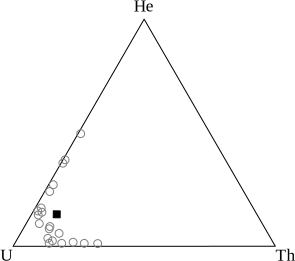
\includegraphics[width=\textwidth]{../figures/ternaryhelium.pdf}\\
\end{minipage}
\begin{minipage}[t]{.6\linewidth}
  \captionof{figure}{The U--Th--He age equation is scale invariant in
    the sense that the three elements can be renormalised to unity
    without loss of chronological information. This figure shows a
    synthetic dataset of 20 scattered U--Th--He measurements (grey
    circles). The arithmetic mean composition of the dataset is shown
    as a black square. It plots outside the data cloud, and is
    therefore not representative of the data.\\}
  \label{fig:ternaryhelium}
\end{minipage}

\citet{aitchison1986} showed that the natural way to process
compositional data is by subjecting them to a \textbf{logratio
  transformation}. In the case of the U--Th--He system, the logratio
analysis is achieved by first defining two new variables:
\begin{equation}
  u \equiv \ln\!\left(\frac{\mbox{[U]}}{\mbox{[He]}}\right),
  v \equiv \ln\!\left(\frac{\mbox{[Th]}}{\mbox{[He]}}\right)
  \label{eq:alr}
\end{equation}

\noindent and then performing the desired statistical analysis
(averaging, uncertainty propagation, ...) on the transformed
data. Upon completion of the mathematical operations, the results can
then be mapped back to U-Th-(Sm)-He space using an inverse logratio
transformation:
\begin{equation}
    [He] = \frac{1}{\left[e^{u}+e^{v}+1\right]},~
    [U] = \frac{e^{u}}{\left[e^{u}+e^{v}+1\right]},~
    [Th] = \frac{e^{v}}{\left[e^{u}+e^{v}+1\right]}
    \label{eq:ialr}
\end{equation}

\noindent where [He] + [U] + [Th] = 1.\\

\noindent\includegraphics[width=\linewidth]{../figures/alr.pdf}
\begingroup
\captionof{figure}{The logratio transformation maps data from an
  $n$-dimensional compositional space to an $(n-1)$-dimensional
  Euclidean space. For the U--Th--He data, it maps the data from a
  ternary diagram ($n=3$) to a bivariate ($n-1=2$) dataspace using
  Equation~\ref{eq:alr}. In this transformed space, it is safe to
  calculate the arithmetic mean (black square) and confidence regions
  (black ellipse). After completion of these calculations, the result
  can be mapped back to the ternary diagram using the inverse logratio
  transformation (Equation~\ref{eq:ialr}).\\}
\label{fig:alr}
\endgroup

In the context of U--Th--He dating, the central age is defined as the
age that corresponds to the arithmetic mean composition in logratio
space. \texttt{IsoplotR}'s \texttt{helioplot} function performs this
calculation using the same algorithm that is used to obtain the
weighted mean U-Pb composition for the concordia age calculation
(Section~\ref{sec:concordia}).\\

\noindent\begin{minipage}[t]{.7\linewidth}
\strut\vspace*{-\baselineskip}\newline
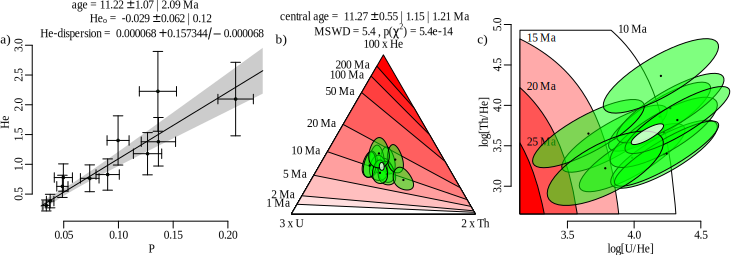
\includegraphics[width=\textwidth]{../figures/helioplot.pdf}\\
\end{minipage}
\begin{minipage}[t]{.3\linewidth}
  \captionof{figure}{a) ternary diagram and b) logratio diagram or
    `helioplot' of the U--Th--He data from
    Figure~\ref{fig:UThHeisochron}. The white ellipse marks the
    average U--Th--He composition.\\}
  \label{fig:UThHeIsochronHelioplot}
\end{minipage}

Overdispersion is treated similarly as in a regression context
(Section~\ref{sec:regression}).  Thus, there are options to augment
the uncertainties with a factor $\sqrt{\mbox{MSWD}}$ (model-1); to
ignore the analytical uncertainties altogether (model-2); or to add an
overdispersion term to the analytical uncertainties (model-3).  The
helioplot diagram provides a convenient way to simultaneously display
the isotopic composition of samples and their chronological
meaning. In this respect, they fulfil the same purpose as the U--Pb
concordia diagram (Section~\ref{sec:concordia}) and the U--series
evolution plot (Section~\ref{sec:ThUevolution}).

\printbibliography[heading=subbibliography]

\end{refsection}


\begin{refsection}

\chapter{Fission tracks}\label{ch:fissiontracks}

\texttt{IsoplotR} accepts three types of fission track data:

\begin{enumerate}
\item{`EDM':} \textzeta, err[\textzeta],
  \textrho\textsubscript{D}, err[\textrho\textsubscript{D}], 
  N\textsubscript{s}, N\textsubscript{i}
\item{`ICP (\textzeta)':} \textzeta, err[\textzeta], spot size
  (\textmu{m}), N\textsubscript{s}, A (\textmu{m}\textsuperscript{2}),
  U\textsubscript{1}, err[U\textsubscript{1}], $\ldots$, U\textsubscript{n},
  err[U\textsubscript{n}]
\item{`ICP (absolute)':} mineral, spot size (\textmu{m}),
  N\textsubscript{s}, A (\textmu{m}\textsuperscript{2}),
  U\textsubscript{1}, err[U\textsubscript{1}], $\ldots$, U\textsubscript{n},
  err[U\textsubscript{n}]
\end{enumerate}

\noindent \textzeta, err[\textzeta], \textrho\textsubscript{D},
err[\textrho\textsubscript{D}], and `spot size' are scalars, whereas
N\textsubscript{s}, N\textsubscript{i}, A, U\textsubscript{i} and
err[U\textsubscript{i}] are vectors. `mineral' is a text string that
either equals \texttt{apatite} or \texttt{zircon}.  The three formats
represent two different approaches to fission track dating:

\begin{enumerate}
\item The External Detector Method \citep[EDM,][]{hurford1983}
  implements the neutron irradiation method that was previously
  introduced in Section~\ref{sec:fission-tracks}.
\item The `ICP' method uses LA-ICP-MS (see
  Section~\ref{sec:mass-specs}) to determine the
  \textsuperscript{238}U-content of fission track samples.  The main
  reasons for this change are the increased throughput achieved by not
  having to irradiate samples and the ease of double-dating apatite
  and zircon with the U-Pb method.
\end{enumerate}

\section{The external detector method}
\label{sec:EDM}

Recall the fission track age equation from
Section~\ref{sec:fission-tracks}:
\begin{equation}
t =
\frac{1}{\lambda_{38}}\ln\left(1+\frac{g_i}{g_s}
\lambda_{38}\zeta\rho_d\frac{N_s}{N_i}\right)
\label{eq:tzeta2}
\end{equation}

The fission track method has been a test bed of statistical approaches
that have subsequently been adopted by other chronometers. A case in
point is the radial plot, which is uniquely suited to deal with the
large and highly variable (`heteroscedastic') counting uncertainties
of fission track data. Spontaneous fission is accurately described by
a Poisson distribution. For young and/or uranium-poor samples, there
is a finite probability that the spontaneous track count is zero for
some grains.  To accommodate such zero values, it is customary to use
an arcsine transformation for radial plots instead of the usual
logarithmic transformation \citep{galbraith1990a}:
\begin{equation}
z_j = \arcsin\sqrt{\frac{N_{sj} + 3/8}{N_{sj}+N_{ij}+3/4}}
\label{eq:zj}
\end{equation}

\noindent and
\begin{equation}
\sigma_j = \frac{1}{2\sqrt{N_{sj}+N_{ij}+1/2}}
\label{eq:sj}
\end{equation}

The arithmetic mean is not a reliable estimator of the true age, for a
similar reason why the arithmetic mean is not the best estimator of
the average U--Th--He composition and age. The Poisson distribution is
positively skewed, and this biases the arithmetic mean. The solution
is similar as for the U--Th--He method, namely:

\begin{enumerate}
\item Take the average logarithm of the spontaneous and induced
  track densities.
\item Compute the fission track age the corresponds to this average
  ratio.
\end{enumerate}

This procedure again gives rise to a `central age'. Fission track data
are often overdispersed with respect to the Poisson counting
uncertainties, and this dispersion carries important thermal history
information. It is therefore customary to compute the average track
density ratio using a model-3 style random effects model, in which the
true $\rho_s/\rho_i$-ratio is assumed to follow a log-normal
distribution with location parameter $\mu$ and scale parameter
$\sigma$ \citep{galbraith1993}:
\begin{equation}
\ln\left[\frac{\rho_s}{\rho_i}\right] \sim \mathcal{N}(\mu,\sigma^2)
\label{eq:logrhosrhoi}
\end{equation}

This model gives rise to a two-parameter log-likelihood function:
\begin{equation}
  \mathcal{L}(\mu,\sigma^2) = \sum\limits_{j=1}^{n}
  \ln f_j(\mu,\sigma^2)
\label{eq:Lcentral}
\end{equation}

\noindent where the probability mass function $f_j(\mu,\sigma^2)$ is
defined as:
\begin{equation}
  f_j(\mu,\sigma^2) = {{N_{sj}+N_{ij}}\choose{N_{sj}}}
  \int\limits_{-\infty}^{\infty} \frac{e^{\beta N_{sj}} \left( 1 +
    e^\beta \right)^{-N_{sj}-N_{ij}}} {\sigma\sqrt{2\pi}
    e^{(\beta-\mu)^2/(2\sigma^2)}} d\beta
  \label{eq:fjms}
\end{equation}

\noindent in which the fission track count ratios are subject to two
sources of variation: the Poisson counting uncertainty and an
`(over)dispersion' factor $\sigma$.  Maximising Eq. \ref{eq:Lcentral}
results in two estimates $\hat{\mu}$ and $\hat{\sigma}$ and their
respective standard errors.  Substituting $\exp[\hat{\mu}]$ for
$N_s/N_i$ in Equation~\ref{eq:tzeta2} produces the desired central
age. $\hat{\sigma}$ estimates the overdispersion, and quantifies the
excess scatter of the single grain ages which cannot be explained by
the Poisson counting statistics alone. This dispersion can be just as
informative as the central age itself, as it encodes geologically
meaningful information about the compositional heterogeneity and
cooling history of the sample.

\section{LA-ICP-MS based fission track dating}
\label{sec:ICPFT}

The EDM continues to be the most widely used analytical protocol in
fission track dating. However, over the past decade, an increasing
number of laboratories have abandoned it and switched to LA-ICP-MS as
a means of determining the uranium concentration of datable minerals,
thus reducing sample turnover time and removing the need to handle
radioactive materials\citep{hasebe2004, chew2012, vermeesch2017}. The
statistical analysis of ICP-MS based FT data is less straightforward
and less well developed than that of the EDM. The latter is based on
simple ratios of Poisson variables, and forms the basis of a large
edifice of statistical methods which cannot be directly applied to
ICP-MS based data. The following paragraphs summarise
\citet{vermeesch2017}'s solution to these issues, as implemented in
\texttt{IsoplotR}.\\

Two analytical approached are being used in ICP-based fission track
geochronology, which each correspond to a different data format:

\begin{enumerate}
\item The `absolute dating' method is based on
  Equation~\ref{eq:tFT}:
  \begin{equation}
    {t} = \frac{1}{\lambda_{38}}
    \ln \left(1 + \frac{\lambda_{38}}{\lambda_f}\frac{N_s}{[{U}] A_s R_e ~ q}\right)
    \label{eq:tICP}
  \end{equation}

  where $N_s$ is the number of spontaneous tracks counted over an area
  $A_s$, $q$ is an `efficiency factor' \citep[$\sim$0.93 for apatite and
    $\sim$1 for
    zircon,][]{iwano1998,enkelmann2003,jonckheere2003b,soares2013} and
  $[{U}]$ is the $^{238}$U-concentration (in atoms per unit volume)
  measured by LA-ICP-MS. Equation \ref{eq:tICP} requires an explicit
  value for $\lambda_f$ and assumes that the etchable range ($R_e$) is
  accurately known \citep{soares2014}.

\item The \textzeta-calibration method folds the etch efficience,
  decay constant and etchable range into a $\zeta$-calibration factor
  akin to that used in the EDM:
  \begin{equation}
    {t} = \frac{1}{\lambda_{38}}
    \ln \left(1+\frac{1}{2}\lambda_{38}{\zeta}_{ICP}\frac{N_s}{A_s[{U}]}\right)
    \label{eq:tzetahatICP}
  \end{equation}

  in which ${\zeta}_{ICP}$ is determined by analysing a standard of
  known FT age \citep{hasebe2004}. Note that, in contrast with the
  `absolute' dating method, the $\zeta$-calibration method allows
  $[{U}]$ to be expressed in any concentration units (e.g., ppm or
  wt\% of total U) or even be replaced with the measured U/Ca-, U/Si-
  or U/Zr-ratios produced by the ICP-MS instrument.
\end{enumerate}

\section{Compositional zoning}\label{sec:zoning}

Uranium-bearing minerals such as apatite and zircon often exhibit
compositional zoning, whose effects must either be removed or
quantified in order to ensure unbiased ages. Two approaches are used
to deal with this issue:

\begin{enumerate}
\item The effect of compositional zoning can be \emph{removed} by
  covering the entire counting area with one large laser spot
  \citep{soares2014} or a raster \citep{hasebe2004}. The uncertainty
  of $[{U}]$ is then simply given by the analytical uncertainty of the
  LA-ICP-MS measurements, which typically is an order of magnitude
  lower than the standard errors of induced track counts in the EDM.
\item Alternatively, the uranium-heterogeneity can be
  \emph{quantified} by analysing multiple spots per analysed grain
  \citep{hasebe2009}. This is why \texttt{IsoplotR} accommodates
  multiple uranium measurements per aliquot (U\textsubscript{1},
  err[U\textsubscript{1}], $\ldots$, U\textsubscript{n},
  err[U\textsubscript{n}])\\

  It is commonly found that the scatter of the different
  uranium-measurements within each grain far exceeds the formal
  analytical uncertainty of each spot measurement. \texttt{IsoplotR}
  assumes that this dispersion is constant across all aliquots and
  follows a log-normal distribution:
  \begin{equation}
    \ln[U_{jk}] \sim \mathcal{N}(\mu_j,\sigma^2+s[U]_{jk}^2)
    \label{eq:lognorm}
  \end{equation}

  where ${U}_{jk}$ is the $k$\textsuperscript{th} (out of $n_j$)
  uranium concentration measurement, $s[U]_{jk}$ is its standard
  error, and $\mu_j$ and $\sigma^2$ are the (unknown) mean and
  variance of a Normal distribution. Note that $\mu_j$ is allowed to
  vary from grain to grain but $\sigma$ is not.  $\mu_j$ and $\sigma$
  can be estimated using the method of maximum likelihood, and the
  corresponding geometric mean uranium concentrations ($\exp[\mu_j]$)
  directly plugged into Equation~\ref{eq:tICP}.
\end{enumerate}

To plot ICP-MS based fission track data on a radial plot, we can
replace Equations~\ref{eq:zj} and \ref{eq:sj} with
\begin{align}
  z_j & = \ln ({t}_j) \mbox{,}   \label{eq:zj2} \\
  \mbox{and~} s_j & = \sqrt{ 
    \left(\frac{s[{\zeta}]}{{\zeta}}\right)^2 +
    \left(\frac{s[{U}]}{{U}}\right)^2 +
    \frac{1}{N_s}
  }   \label{eq:sj2}
\end{align}

respectively \citep{galbraith2010b}. Alternatively, a square root
transformation may be more appropriate for young and/or U-poor
samples:
\begin{align}
  z_j & = \sqrt{{t}_j} \mbox{,}   \label{eq:zj3} \\
  \mbox{and~} s_j & = s[{t}_j]\bigg/\left(2\sqrt{{t}_j}\right)
  \label{eq:sj3}
\end{align}

\noindent\includegraphics[width=\linewidth]{../figures/FTradial.pdf}
\begingroup \captionof{figure}{Radial plots of EDM-based fission track
  data using the a) logarithmic and b) arcsine transformation; and of
  ICP-based fission track data using the c) logarithmic and d) square
  root transformation.}  \endgroup

\section{Zero track counts}
\label{sec:zeroICP}

The standard error of a single grain fission track age estimate can be
derived by standard error propagation.  For the EDM, this yields:
\begin{equation}
s[{t}] \approx {t} \sqrt{ 
  \left(\frac{s[{\zeta}]}{{\zeta}}\right)^2 +
  \left(\frac{s[{\rho_D}]}{{\rho_D}}\right)^2 +
  \frac{1}{N_s} + \frac{1}{N_i}
}
\label{eq:stEDM}
\end{equation}

\noindent which returns an infinite uncertainty if either $N_s$ or
$N_i$ is zero. For the EDM, this problem is adequately addressed by
adding half a count to both the spontaneous and induced track count:
\begin{equation}
s[{t}] \approx {t} \sqrt{ 
  \left(\frac{s[{\zeta}]}{{\zeta}}\right)^2 +
  \left(\frac{s[{\rho_D}]}{{\rho_D}}\right)^2 +
  \frac{1}{N_s+\frac{1}{2}} + \frac{1}{N_i+\frac{1}{2}}
}
\label{eq:stEDM0}
\end{equation}

This correction avoids the problem with zero or small counts whilt
only having a minor effect on the accuracy of the
estimate. Unfortunately this simple trick does not work for ICP-based
fission track data, whose uncertainty estimates are given by (for the
absolute dating approach):
\begin{equation}
s[{t}] \approx {t} \sqrt{ 
  \left(\frac{s[{U}]}{{U}}\right)^2 +
  \frac{1}{N_s}
}
\label{eq:shatt4}
\end{equation}

Adding half a count to the spontaneous fission track count would bias
the data to a greater or lesser degree depending on whether the grain
is poor or rich in uranium. One pragmatic solution to this problem is
to approximate the ICP-MS based uranium concentration measurement with
an `equivalent induced track density', using the following linear
transformation:
\begin{equation}
\hat{N}_{ij} = \rho_j A_{sj} [{U}_j]
\end{equation}

\noindent where $A_{sj}$ is the area over which the spontaneous tracks
of the j$^{th}$ grain have been counted and $\rho_j$ plays a similar
role as $\rho_d$ in Eq.~\ref{eq:tzeta}. From the requirement that the
variance of a Poisson-distributed variable equals its mean, it follows
that:
\begin{equation}
\hat{N}_{ij} = \rho_j^2 A_{sj}^2 s[{U}_j]^2
\end{equation}

\noindent from which it is easy to determine $\rho_j$. Thus the ICP-MS
data have effectively been converted in to EDM data, and can be
subjected to the same treatment as EDM data.

\printbibliography[heading=subbibliography]

\end{refsection}


\begin{refsection}

\chapter{\textsuperscript{230}Th--U}\label{ch:ThU}

The general principles of U-series disequilibrium dating were laid out
in Chapter~\ref{ch:intro2Useries}. Recall that the radioactive decay
of \textsuperscript{238}U to \textsuperscript{206}Pb produces
short-lived \textsuperscript{230}Th (t\textsubscript{1/2}=76~kyr) and
\textsuperscript{234}U (t\textsubscript{1/2}=246~kyr), which may
fractionate by one of several mechanisms:

\begin{enumerate}
\item U and Th have contrasting chemical properties and are easily
  fractionated during chemical processes such as crystallisation. This
  fractionation disrupts any pre-existing state of secular equilibrium
  between \textsuperscript{230}Th and its parent nuclide
  \textsuperscript{234}U.
\item Preferential leaching of weakly sited \textsuperscript{234}U due
  to energetic recoil of the U-nucleus during
  \textsuperscript{238}U-decay enriches \textsuperscript{234}U
  relative to \textsuperscript{238}U in river and sea water.
\item Redox processes and repeated precipitation--dissolution cycles
  may fractionate \textsuperscript{234}U from \textsuperscript{238}U,
  especially in the presence of organic acids in soils. This can
  produce ground waters that are highly enriched in
  \textsuperscript{234}U relative to \textsuperscript{238}U.
\end{enumerate}

Section~\ref{sec:234238} showed that the fractionation between
\textsuperscript{234}U and \textsuperscript{238}U can be used to date
marine carbonates; Section~\ref{sec:230} showed that the fractionation
between \textsuperscript{230}Th and \textsuperscript{234}U can be used
to date young volcanic rocks; and Section~\ref{sec:230238} combined
the two equations together in a single equation. Recall
Equation~\ref{eq:230238}:
\begin{equation*}
  \frac{A(^{230}Th)}{A(^{238}U)} = 1 - e^{-\lambda_{230}t} +
  \frac{\lambda_{230}}{\lambda_{230}-\lambda_{234}} (\gamma_\circ-1)
\left(e^{-\lambda_{234}t}-e^{-\lambda_{230}t}\right)
\end{equation*}

\noindent where $A[\ast]$ is the activity of $\ast$ and $\gamma_\circ$
is the oceanic \textsuperscript{234}U/\textsuperscript{238}U activity
ratio. This equation requires that $\gamma_\circ$ is known and
produces non-unique age solutions when
A(\textsuperscript{230}Th)/A(\textsuperscript{238}U)$>1$. Both of
these limitations can be avoided by recasting the equation into the
following form:
\begin{equation}
  \begin{split}
  & \frac{A[{}^{230}Th] - A[{}^{230}Th]_{\circ}e^{-\lambda_{230}t}}{A[{}^{238}U]} = \\
  & 1 - e^{\lambda_{230}t} -
  \left(\frac{A[{}^{234}U]}{A[{}^{238}U]}-1\right)
  \left(\frac{\lambda_{230}}{\lambda_{234}-\lambda_{230}}\right)
  \left(1-e^{[\lambda_{234}-\lambda_{230}]t}\right)
  \end{split}
  \label{eq:Th-U}
\end{equation}

\noindent where $A[{}^{230}Th]_\circ$ is the `detrital' \textsuperscript{230}Th
component, i.e. the \textsuperscript{230}Th that was already present
in the sample at the time of its formation \citep{kaufman1965,
  ludwig2003b}. This component is unknown but can be estimated by
isochron regression using long-lived \textsuperscript{232}Th as a
normalising factor.\\

\texttt{IsoplotR} uses Equation~\ref{eq:Th-U} as the basis of all its
U-series dating applications.

\section{Data formats}\label{sec:ThUformats}

\texttt{IsoplotR} accepts U-series data in four different formats:

\begin{enumerate}
\item $\frac{38}{32}$, $s\!\left[\frac{38}{32}\right]$,
  $\frac{34}{32}$, $s\!\left[\frac{34}{32}\right]$,
  $\frac{30}{32}$, $s\!\left[\frac{30}{32}\right]$,
  $r\!\left[\frac{38}{32},\frac{34}{32}\right]$,
  $r\!\left[\frac{38}{32},\frac{30}{32}\right]$,
  $r\!\left[\frac{34}{32},\frac{30}{32}\right]$
\item $\frac{32}{38}$, $s\!\left[\frac{32}{38}\right]$,
  $\frac{34}{38}$, $s\!\left[\frac{34}{38}\right]$,
  $\frac{30}{38}$, $s\!\left[\frac{30}{38}\right]$,
  $r\!\left[\frac{32}{38},\frac{34}{38}\right]$,
  $r\!\left[\frac{32}{38},\frac{30}{38}\right]$,
  $r\!\left[\frac{34}{38},\frac{30}{38}\right]$
\item $\frac{38}{32}$, $s\!\left[\frac{38}{32}\right]$,
  $\frac{30}{32}$, $s\!\left[\frac{30}{32}\right]$,
  $r\!\left[\frac{38}{32},\frac{30}{32}\right]$
\item $\frac{32}{38}$, $s\!\left[\frac{32}{38}\right]$,
  $\frac{30}{38}$, $s\!\left[\frac{30}{38}\right]$,
  $r\!\left[\frac{32}{38},\frac{30}{38}\right]$
\end{enumerate}

\noindent where `30', `32', `34' and `38' stand for
\textsuperscript{230}Th, \textsuperscript{232}Th,
\textsuperscript{234}U and \textsuperscript{238}U, respectively.  It
is important to emphasise that, unlike all of \texttt{IsoplotR}'s
other data formats, the numbers in these data tables are no atomic
ratios but activity ratios. The relationship between activity ratios
and atomic ratios is given by:
\begin{equation}
  \frac{A(x)}{A(y)} \equiv 
  \frac{\mbox{activity}(x)}{\mbox{activity}(y)} =
  \frac{\mbox{atoms}(x)}{\mbox{atoms}(y)}
  \frac{\lambda_{x}}{\lambda_{y}}
\end{equation}

Formats~1 and 2 are applicable to carbonate lithologies in which both
the \textsuperscript{230}Th/\textsuperscript{234}U and
\textsuperscript{234}U/\textsuperscript{238}U equilibrium have been
disturbed. Formats~3 and 4 are applicable to igneous rocks, in which
only the \textsuperscript{230}Th/\textsuperscript{234}U activity ratio
has been distrubed, but \textsuperscript{234}U and
\textsuperscript{238}U are in secular equilibrium (see
Section~\ref{sec:230}).

The error correlations of formats~1 and 3 tend to be stronger than
those of formats~2 and 4. This is because formats~1 and 3 normalise
the elements of the \textsuperscript{238}U decay series to the highly
variable amount of detrital \textsuperscript{232}Th. In contrast,
formats~2 and 4 feature only one ratio containing
\textsuperscript{232}Th, thus reducing a source of shared variability.

\section{Isochrons}

For igneous samples, in which $A[{}^{234}U]/A[{}^{238}U] = 1$, the
second term on the right-hand side of Equation~\ref{eq:Th-U} vanishes
and we can write:
\begin{equation}
  \left(\frac{A[{}^{230}Th]}{A[{}^{232}Th]}\right)_i = 
  \left(\frac{A[{}^{230}Th]}{A[{}^{232}Th]}\right)_{\!\circ}
  e^{-\lambda_{230}t} +
  \left(\frac{A[{}^{238}U]}{A[{}^{232}Th]}\right)_i
  \left(1-e^{-\lambda_{230}t}\right)
  \label{eq:rosholt}
\end{equation}

\noindent for $1 \leq i \leq n$, which can be solved for $t$ and
$\left(A[{}^{230}Th]/A[{}^{232}Th]\right)_{\!\circ}$ using the least
squares method of \citet{york2004}. Equation~\ref{eq:rosholt} (which
was previously derived as Equation~\ref{eq:230232}) forms a
`Rosholt'-type isochron, which is akin to a conventional isochron in
Rb--Sr or Ar--Ar geochronology \citep{rosholt1976}. Using
$A[{}^{238}U]$ as the normalising factor instead yields an
`Osmond'-type isochron, which is akin to an inverse isochron in Ar--Ar
or Pb--Pb geochronology \citep{osmond1970, ludwig2003b}:
\begin{equation}
  \left(\frac{A[{}^{230}Th]}{A[{}^{238}U]}\right)_i =
  \left(1-e^{\lambda_{230}t}\right) +
  \left(\frac{A[{}^{232}Th]}{A[{}^{238}U]}\right)_i
  \left(\frac{A[{}^{230}Th]}{A[{}^{232}Th]}\right)_\circ
  e^{-\lambda_{230}t}
  \label{eq:osmond}
\end{equation}

Note that for the Rosholt isochron, the age is a function of the
slope, whereas for the Osmond isochron, it is a function of the
y-intercept.\\

For carbonate samples, in which \textsuperscript{234}U and
\textsuperscript{238}U generally are not in secular equilibrium, three
activity ratios are needed to determine the detrital
\textsuperscript{230}Th (and initial \textsuperscript{234}U)
component. This in turn requires three dimensional isochron regression
of the \textsuperscript{230}Th/\textsuperscript{238}U-,
\textsuperscript{232}Th/\textsuperscript{238}U- and
\textsuperscript{234}U/\textsuperscript{238}U-activity
ratios. \texttt{IsoplotR} performs this calculation using the maximum
likelihood algorithm of \citet{ludwig1994}. This solves the following
system of equations\footnote{The same calculations can also be
performed in `Rosholt space', with \textsuperscript{232}Th as a common
denominator, but an in-depth discussion of this is omitted for the
sake of brevity.}:
\begin{equation}
  \begin{cases}
    \left[\frac{{}^{234}\mbox{U}}{{}^{238}\mbox{U}}\right]_i =
    a + b \left[\frac{{}^{232}\mbox{Th}}{{}^{238}\mbox{U}}\right]_i +
    \delta_i \\
    \left[\frac{{}^{230}\mbox{Th}}{{}^{238}\mbox{U}}\right]_i =
    \alpha + \beta \left[\frac{{}^{232}\mbox{Th}}{{}^{238}\mbox{U}}\right]_i +
    \epsilon_i
  \end{cases}
  \label{eq:titterington}
\end{equation}

\noindent where $\delta_i$ and $\epsilon_i$ are the bivariate normal
residuals. Equation~\ref{eq:titterington} can be solved by maximising
the following log-likelihood function for $x_i$, $a$, $b$, $\alpha$
and $\beta$:
\begin{equation}
  \mathcal{LL} = \mbox{const.} - 
  \frac{1}{2} \sum\limits_{i=1}^{n}
  \left[
    \begin{array}{@{}c@{}}
      \left[\frac{32}{38}\right]_{\!i} - x_{i} \\
      \left[\frac{34}{38}\right]_{\!i} - a - b x_{i} \\
      \left[\frac{30}{38}\right]_{\!i} - \alpha - \beta x_{i}
    \end{array}
    \right]^T
  \left[
    \begin{array}{@{}c@{~}c@{~}c@{}}
      s\!\left[\frac{32}{38}\right]_{\!i}^2 &
      s\!\left[\frac{32}{38},\frac{34}{38}\right]_{\!i} &
      s\!\left[\frac{32}{38},\frac{30}{38}\right]_{\!i} \\
      s\!\left[\frac{34}{38},\frac{32}{38}\right]_{\!i} &
      s\!\left[\frac{34}{38}\right]_{\!i}^2 &
      s\!\left[\frac{34}{38},\frac{30}{38}\right]_{\!i} \\
      s\!\left[\frac{30}{38},\frac{32}{38}\right]_{\!i} &
      s\!\left[\frac{30}{38},\frac{34}{38}\right]_{\!i} &
      s\!\left[\frac{30}{38}\right]_{\!i}^2
    \end{array}
    \right]^{-1}
  \left[
    \begin{array}{@{}c@{}}
      \left[\frac{32}{38}\right]_{\!i} - x_{\!i} \\
      \left[\frac{34}{38}\right]_{\!i} - a - b x_{i} \\
      \left[\frac{30}{38}\right]_{\!i} - A - B x_{i}
    \end{array}
    \right]
\end{equation}

\noindent which uses the shorthand notation introduced at the
beginning of Section~\ref{sec:ThUformats}. The isochron age can be
obtained by substituting the estimate of $a$ for
$\left[\frac{{}^{234}\mbox{U}}{{}^{238}\mbox{U}}\right]_i$ and
$\alpha$ for
$\left[\frac{{}^{230}\mbox{Th}}{{}^{238}\mbox{U}}\right]_i$ in
Equation~\ref{eq:Th-U}, and setting $A[{}^{230}Th]_{\circ}=0$.
Additionally, the fit parameters ($a$, $b$, $\alpha$ and $\beta$) can
also be used to estimate the following quantities:

\begin{enumerate}
\item{(\textsuperscript{234}U/\textsuperscript{238}U)\textsubscript{0}} $=a$:
  the authigenic \textsuperscript{234}U/\textsuperscript{238}U
  activity ratio;
\item{(\textsuperscript{230}Th/\textsuperscript{232}Th)\textsubscript{0}}
  $=\beta$: the authigenic
  \textsuperscript{230}Th/\textsuperscript{232}Th activity ratio;
\item{(\textsuperscript{230}Th/\textsuperscript{238}U)\textsubscript{0}}
  $=\alpha$: the detrital
  \textsuperscript{230}Th/\textsuperscript{238}U activity ratio;
\item{(\textsuperscript{234}U/\textsuperscript{238}U)\textsubscript{i}}
  = $1 + (a-1)e^{\lambda_{234}t}$: the initial
  \textsuperscript{234}U/\textsuperscript{238}U activity ratio.
\end{enumerate}

The results of the three-dimensional isochron regression can be
visualised in four possible ways:

\noindent\begin{minipage}[t][][b]{.65\linewidth}
\includegraphics[width=\textwidth]{../figures/ThUisochron.pdf}
\end{minipage}
\begin{minipage}[t][][t]{.35\linewidth}
  \captionof{figure}{The same \textsuperscript{230}Th--U data shown on
    a) Rosholt type-I, b) Osmond type-I, c) Rosholt type-II and d)
    Osmond type-II isochron diagrams. Note the slight difference in
    the isochron age. This is due to the skewness of the uncertainty
    distribution, which does not allow negative values.  This effect
    applies to all isochrons and is most prominent when the analytical
    uncertainties are relatively large compared to the activity ratios
    themselves. Solving this issue requires a reformulation of the
    isochron equation in terms of log-ratios, which has not yet been
    attempted.}
  \label{fig:ThUisochron}
\end{minipage}

\section{Th--U evolution diagrams}\label{sec:ThUevolution}

In addition to (Rosholt and Osmond) isochrons and the usual weighted
mean, radial, CAD and KDE plots, U-series data can also be visualised
on Th-U evolution diagrams.  For carbonate data, these consist of a
scatter plot that sets out the
\textsuperscript{234}U/\textsuperscript{238}U-activity ratios against
the \textsuperscript{230}Th/\textsuperscript{238}U-activity ratios as
error ellipses, and displays the authigenic
\textsuperscript{234}U/\textsuperscript{238}U-activity ratios and ages
as a set of intersecting lines.\\

The Th-U evolution diagram has a similar purpose and appearance as the
U-Pb concordia diagram (Section~\ref{sec:concordia}), which also
displays compositions and dates simultaneously. An alternative way of
doing so for carbonate samples is by plotting the initial
\textsuperscript{234}U/\textsuperscript{238}U-ratios against the
\textsuperscript{230}Th--\textsuperscript{234}U--\textsuperscript{238}U-ages.
In both types of evolution diagrams, \texttt{IsoplotR} provides the
option to project the raw measurements along the best fitting isochron
line and thereby remove the detrital
\textsuperscript{230}Th-component. This procedure allows a visual
assessment of the degree of homogeneity within a dataset, as
quantified by the MSWD.\medskip

\noindent
\includegraphics[width=\linewidth]{../figures/evolution12.pdf}
\captionof{figure}{The data of Figure~\ref{fig:ThUisochron}
  visualised on a \textsuperscript{230}Th--U evolution diagram a)
  showing the raw data with an isochron fit and the inferred
  authigenic end member composition shown as a white ellipse; and b)
  showing the data projected along the isochron.  c) shows the
  projected data in initial
  \textsuperscript{234}U/\textsuperscript{238}U-activity
  vs. \textsuperscript{230}Th--U age space.\medskip}
\label{fig:evolution12}

Neither the U-series evolution diagram nor the
\textsuperscript{234}U/\textsuperscript{238}U vs. age plot is
applicable to igneous datasets, in which \textsuperscript{234}U and
\textsuperscript{238}U are in secular equilibrium.  For such datasets,
\texttt{IsoplotR} produces an Rosholt type-I style regression plot
that is decorated with a fanning set of isochron lines.\medskip

\noindent\begin{minipage}[t][][b]{.7\linewidth}
\includegraphics[width=\textwidth]{../figures/evolution34.pdf}
\end{minipage}
\begin{minipage}[t][][t]{.29\linewidth}
  \captionof{figure}{ An evolution diagram of data formats~3 and 4
    plots the data in Rosholt type-I space with isochrons shown in
    salmon red a) without detrital \textsuperscript{230}Th correction;
    and b) using a whole rock U/Th activity ratio of 2 to estimate the
    \textsuperscript{230}Th/\textsuperscript{238}U isochron ratios.}
  \label{fig:evolution34}
\end{minipage}

\printbibliography[heading=subbibliography]

\end{refsection}


\begin{refsection}

\chapter{Detrital geochronology}\label{ch:detrital}

\section{Maximum depositional age estimation}

\section{Multi-sample plots}

\section{Multidimensional scaling}

\section{Provenance analysis}

\printbibliography[heading=subbibliography]

\end{refsection}


\part{\texttt{IsoplotR} manual}

\begin{refsection}
\chapter{Introduction to \texttt{IsoplotR}}
\label{ch:intro2IsoplotR}
  
For many years, a \texttt{Microsoft Excel} add-in called
\texttt{Isoplot} has been the main data processing software of choice
in geochronology. Developed by Kenneth R. Ludwig over a period of two
decades, \texttt{Isoplot} is a user-friendly toolbox that allows
geologists to calculate and visualise geochronological data within a
familiar spreadsheet environment \citep{ludwig1988, ludwig1999,
  ludwig2003, ludwig2012}.  Few computer programs have been as widely
used in the Earth Sciences as \texttt{Isoplot}. Written in Visual
Basic for Applications (\texttt{VBA}), \texttt{Isoplot} takes isotopic
data as input and produces publication-ready figures as output.\\

Unfortunately, recent versions of \texttt{Excel} are incompatible with
\texttt{Isoplot}, whose creator has retired and no longer maintains
the code. These software issues are a major problem for the field of
radiometric geochronology, to the point where some laboratories kept
an old \texttt{Windows~XP} computer with \texttt{Excel~2003} around
for the sole purpose of running \texttt{Isoplot}.\\

\texttt{IsoplotR} is a free, open and more future proof alternative
for \texttt{Isoplot} \citep{vermeesch2018c}.  \texttt{IsoplotR}'s
software architecture uses a modular design with future proofness and
extendability in mind.

\section{Software architecture}
\label{sec:architecture}

There are three ways to use \texttt{IsoplotR}: online, offline and
from the command line.\\

The online
version\footnote{\texttt{http://isoplotr.london-geochron.com/}} is
convenient in several ways. First, it requires no software
installation. Second, the \texttt{IsoplotR} website is perfectly
platform-independent. It renders on any modern HTML-5 compatible web
browser, including those installed on smartphones and tablet
computers. Third, by using the online version, the user is guaranteed
to have accessed the most up-to-date version of the software.\\

An offline version of the GUI is provided for use on computers that
are not (permanently) connected to the internet. This is often the
case for machines that are connected to mass spectrometers, as a
safety precaution. The offline version of the GUI works by emulating a
web server within the default browser on the user's
system. Installation instructions are provided on the
\texttt{IsoplotR} website and on
\texttt{GitHub}\footnote{\texttt{https://github.com/pvermees/IsoplotRgui/}}.\\

The third way to access the full functionality of \texttt{IsoplotR} is
through the command line within the \texttt{R} programming
environment. The command line offers the greatest flexibility to
automate, modify and extend \texttt{IsoplotR}'s functionality.

\section{The Graphical User Interface (GUI)}
\label{sec:GUI}

The code base for the GUI and the core data processing algorithms are
surgically separated. The command-line functionality is grouped in a
lightweight package called \texttt{IsoplotR} that may be installed
from CRAN as instructed in
Section~\ref{sec:R}.\ref{it:installingIsoplotR}. The \texttt{IsoplotR}
package has minimal dependencies and should work on a basic \texttt{R}
installation. In contrast, the GUI is written in \texttt{HTML} and
\texttt{Javascript} and interacts with \texttt{IsoplotR} via an
interface package. It is provided in a second \texttt{R} package
called \texttt{IsoplotRgui} that is available from CRAN as well:

\begin{verbatim}
install.packages('IsoplotRgui')
\end{verbatim}

Once installed, \texttt{IsoplotRgui} can be started from the
\texttt{R} console as follows:

\begin{verbatim}
library(IsoplotRgui)
\end{verbatim}

This opens the GUI in a new tab of the user's default internet
browser.  The GUI has four components: a top bar with selection menus
for the various chronometers and plot devices, optional settings and
documentation; an input table into which data can be pasted from
spreadsheet applications; an output window displaying the graphical or
numerical results; and a lower bar to import and export data and
results:\\

\noindent\includegraphics[width=\textwidth]{../figures/IsoplotR.png}\\

\noindent\begin{minipage}[t]{.15\textwidth}
\strut\vspace*{-\baselineskip}\newline
  \includegraphics[width=.7\linewidth]{../figures/chronometerbutton.png}
\end{minipage}
\begin{minipage}[t]{.85\textwidth}
IsoplotR currently implements 12 different geochronometers: U--Pb,
Pb--Pb, Th--Pb, Ar--Ar, K--Ca, Rb--Sr, Sm--Nd, Re--Os, Lu--Hf,
U--Th--He, fission tracks, and Th--U.  Additionally, it also includes
functionality for detrital geochronology and general purpose data
processing.\\
\end{minipage}

\noindent\begin{minipage}[t]{.15\textwidth}
\strut\vspace*{-\baselineskip}\newline
\includegraphics[width=\textwidth]{../figures/plotdevices.png}
\end{minipage}
\begin{minipage}[t]{.85\textwidth}
For each chronometer there are several possible plot devices.  These
may vary from method to method. For example, concordia plots are only
available for U--Pb data, and release spectra for Ar--Ar data.\\
\end{minipage}

\noindent\begin{minipage}[t]{.15\textwidth}
\strut\vspace*{-\baselineskip}\newline
\includegraphics[width=.7\textwidth]{../figures/Options.png}
\end{minipage}
\begin{minipage}[t]{.85\textwidth}
The \texttt{Options} menu allows the user to choose between different
input formats and change parameters (e.g. decay constants, plot
colours) that affect the numerical or graphical output.\\
\end{minipage}

\noindent\begin{minipage}[t]{.15\textwidth}
\strut\vspace*{-\baselineskip}\newline
\includegraphics[width=.55\textwidth]{../figures/Help.png}
\end{minipage}
\begin{minipage}[t]{.85\textwidth}
The \texttt{Help} button provides further information about the input
table, about the graphical and numerical numerical results, and some
references. The \texttt{Help} function dynamically responds to the
settings that are listed under the \texttt{Options} menu.\\
\end{minipage}

\noindent\begin{minipage}[t]{.15\textwidth}
\strut\vspace*{-\baselineskip}\newline
\includegraphics[width=.55\textwidth]{../figures/Open.png}\\
\includegraphics[width=.55\textwidth]{../figures/Save.png}\\
\end{minipage}
\begin{minipage}[t]{.85\textwidth}
The data and settings can be stored in a \texttt{.json} format for
further processing in the future.\\
\end{minipage}

\noindent\begin{minipage}[t]{.15\textwidth}
\strut\vspace*{-\baselineskip}\newline
\includegraphics[width=.55\textwidth]{../figures/PLOT.png}\\
\includegraphics[width=.55\textwidth]{../figures/RUN.png}\\
\end{minipage}
\begin{minipage}[t]{.85\textwidth}
The \texttt{PLOT} button (or \texttt{RUN} button if \texttt{ages} or
`\texttt{get $\zeta$}' is chosen as output) saves all the current
settings and produces the graphical and/or numerical output.\\
\end{minipage}

\noindent\begin{minipage}[t]{.15\textwidth}
\strut\vspace*{-\baselineskip}\newline
\includegraphics[width=.55\textwidth]{../figures/PDF.png}\\
\includegraphics[width=.55\textwidth]{../figures/CSV.png}\\
\end{minipage}
\begin{minipage}[t]{.85\textwidth}
Clicking the \texttt{PDF} button repeats the calculations but saves
the output as a \texttt{.pdf} file, which can be further processed by
vector editing software such as \texttt{Adobe Illustrator},
\texttt{CorelDraw} or \texttt{Inkscape}. If \texttt{ages} is chosen as
output saves the results to a comma separated value (\texttt{.csv})
file.\\
\end{minipage}

\noindent\begin{minipage}[t]{.15\textwidth}
\strut\vspace*{-\baselineskip}\newline
\includegraphics[width=.55\textwidth]{../figures/C.png}\\
\end{minipage}
\begin{minipage}[t]{.85\textwidth}
The \texttt{(C)} column of the input table can be used to store
numerical values that can be used as a fill colour for the plot
symbols.\\
\end{minipage}

\noindent\begin{minipage}[t]{.15\textwidth}
\strut\vspace*{-\baselineskip}\newline
\includegraphics[width=.55\textwidth]{../figures/omit.png}
\end{minipage}
\begin{minipage}[t]{.85\textwidth}
Specific samples can be omitted from the numerical calculations
(e.g. isochron, weighted mean, or concordia age) by marking them with
a lowercase `x' in the optional \texttt{(omit)} column. To hide
samples from the graphical (as well as the numerical) output, mark
them with an uppercase `X'.\\
\end{minipage}

\noindent\begin{minipage}[t]{.25\textwidth}
\strut\vspace*{-\baselineskip}\newline
\includegraphics[width=\textwidth]{../figures/formats.png}
\end{minipage}
\begin{minipage}[t]{.75\textwidth}
The \texttt{Options} menu provides access to a range of different
input formats. Selecting any item from this menu replaces the input
table with a different set of default data.\\
\end{minipage}

\noindent\begin{minipage}[t]{.25\textwidth}
\strut\vspace*{-\baselineskip}\newline
\includegraphics[width=.85\textwidth]{../figures/ierr.png}
\end{minipage}
\begin{minipage}[t]{.75\textwidth}
The \texttt{Options} menu also allows the user to specify the ratio
uncertainties as being absolute or relative errors at 1 or 2 standard
errors. Selecting any item from this menu automatically changes the
input data accordingly.\\
\end{minipage}

\noindent\begin{minipage}[t]{.25\textwidth}
\strut\vspace*{-\baselineskip}\newline
\includegraphics[width=.85\textwidth]{../figures/ierr.png}\\
\end{minipage}
\begin{minipage}[t]{.75\textwidth}
Contextual help can be obtained by clicking any text string within the
\texttt{Options} menu.
\end{minipage}

\noindent\begin{minipage}[t]{.45\textwidth}
\strut\vspace*{-\baselineskip}\newline
\includegraphics[width=\textwidth]{../figures/contextualhelp.png}
\end{minipage}
\begin{minipage}[t]{.55\textwidth}
Contextual help can be obtained by clicking any text string within the
\texttt{Options} menu.
\end{minipage}

\section{The Command Line Interface (CLI)}

CLI offers all the functionality of the GUI, and more. A complete list
of public functions can be viewed by typing

\begin{verbatim}
help(package='IsoplotR')
\end{verbatim}

\noindent at the command prompt. Data are read from comma-separated
variable (\texttt{.csv}) files using the \texttt{read.data()}
function. For example:

\begin{verbatim}
UPb_dat <- read.data('file.csv',method='U-Pb',format=1,ierr=3)
\end{verbatim}

\noindent where\\

\noindent\begin{tabular}{@{}p{.2\textwidth}@{}p{.04\textwidth}@{}p{.76\textwidth}@{}}
\verb|'file.csv'| && is the name of the data file\\
\verb|method='U-Pb'| && specifies the chronometer\\
\verb|format=1| && tells \texttt{IsoplotR} that \verb|file.csv|
contains the following columns: \textsuperscript{207}Pb/\textsuperscript{235}U,
err[\textsuperscript{207}Pb/\textsuperscript{235}U],
\textsuperscript{206}Pb/\textsuperscript{238}U,
err[\textsuperscript{206}Pb/\textsuperscript{238}U], and
$r$, where `err[*]' marks the uncertainties of `*', and $r$ is
the correlation coefficient between
err[\textsuperscript{207}Pb/\textsuperscript{235}U]
and err[\textsuperscript{206}Pb/\textsuperscript{238}U]
(see Chapter~\ref{ch:formats}).\\
\verb|ierr=3| && indicates that these uncertainties (`err[*]') are specified
as relative values at two standard errors.
\end{tabular}\\

\noindent Further details about these arguments can be viewed by
typing \texttt{?read.data} at the console. The various plot devices
are implemented in a collection of designated functions such as
\texttt{concordia()}, \texttt{isochron()}, \texttt{weightedmean()},
\texttt{isochron()}, \texttt{agespectrum()}, \texttt{KDE()},
\texttt{CAD()} and \texttt{radialplot()} that will be discussed in
further details in later chapters. A table of age estimates can be
obtained using the \texttt{ages()} function. Many of
\texttt{IsoplotR}'s functions are \emph{overloaded}, which means that
the same function can be applied to multiple data types with
potentially different results. For example, using the output of
\verb|read.data('data.csv',method='Rb-Sr')| as input to the
\texttt{isochron()} function automatically produces a Rb--Sr isochron,
with the correct decay constants and axis labels.\\

A colour scale can be added to most plots using the options
\texttt{levels} argument. For example:

\begin{verbatim}
ns <- length(UPb_dat)
concordia(UPb_dat,levels=runif(ns),
          ellipse.fill=c("yellow","red")
\end{verbatim}

\noindent assigns a vector of random numbers to some U--Pb data and
uses these numbers to colour the error ellipses on a concordia diagram
from yellow to red. Omitting or hiding samples from calculations
and/or plots is achieved by specifying the indices of the relevant
aliquots to the functions of interest. For example:

\begin{verbatim}
weightedmean(UPb_dat,omit=10)
\end{verbatim}

\noindent omits the 10\textsuperscript{th} from the weighted mean
calculation, whereas

\begin{verbatim}
weightedmean(UPb_dat,hide=10)
\end{verbatim}

\noindent removes the aliquot from the weighted mean diagram
altogether.

The GUI may be the easiest way to interact with \texttt{IsoplotR} and
explore various data processing strategies with individual
samples. But the CLI is more useful than the GUI when processing large
datasets comprising multiple samples, and provides a powerful
mechanism to produce \emph{reproducible} science. The \texttt{.csv}
data files and \texttt{.R} data processing scripts can easily be
archived and shared with others. They provide a parsimonious way to
produce FAIR science \citep{wilkinson2016}.

\section{General purpose functions}

\printbibliography[heading=subbibliography]

\end{refsection}


\begin{refsection}

\chapter{Generic functions}
\label{ch:generic-R}

\noindent\begin{minipage}[t]{.3\linewidth}
\strut\vspace*{-\baselineskip}\newline
\includegraphics[width=\linewidth]{../figures/OtherMethodsPlotdevices.png}\\
\end{minipage}
\begin{minipage}[t]{.7\textwidth}
  \texttt{IsoplotR} implements a number of plotting devices for 13
  different geochronometric methods. Some of these plotting devices
  are shared by multiple chronometers, and can also be used for
  datasets of non geochronological origin. This tutorial will start
  with an overview of these `generic' plots, whose user interface is
  shared by all the specific geochronological implementations that
  will be introduced subsequently.
\end{minipage}

In this Chapter, we will use a number of \texttt{IsoplotR}'s built-in
datasets, which can be downloaded from the \texttt{IsoplotR} GitHub
page, at \url{https://tinyurl.com/IsoplotRdata}. For the tutorial in
this Chapter, we will use the following datasets:

\begin{script}
data1 <- read.data('MountTom.csv',method='other')
data2 <- read.data('regression.csv',method='other')
data3 <- read.data('LudwigMean.csv',method='other')
data4 <- read.data('LudwigSpectrum.csv',method='other')
data5 <- read.data('LudwigKDE.csv',method='other')
\end{script}

Alternatively, the same files can also be found in the
\texttt{IsoplotR} installation folder on your computer, using
\texttt{R}'s built-in \texttt{system.file()} function. For example:

\begin{script}
fn <- system.file('MountTom.csv',package='IsoplotR')
data1 <- read.data(fn,method='other')
\end{script}

\section{Radial plots}\label{sec:OtherRadial}

\noindent\begin{minipage}[t]{.27\linewidth}
  \strut\vspace*{-\baselineskip}\newline
  \includegraphics[width=\linewidth]{../figures/OtherRadialInput.png}
\end{minipage}
\begin{minipage}[t]{.73\linewidth}
  Radial plots require a table of measurements and their
  uncertainties, plus an optional vector with data that can be used to
  form a colour scale, and an optional list of data points to omit
  from the calculations or hide from the plot (see
  Sections~\ref{sec:GUI} and \ref{sec:CLI}).
\end{minipage}

\begin{console}
radialplot(data1)
\end{console}

The standard radial plot can be modified using a range of optional
arguments, which can be accessed from the GUI and CLI.

\begin{enumerate}

\item Labelling the error ellipses can be useful to identify outliers
  or otherwise noteworthy aliquots.

  \noindent\begin{minipage}[t]{.28\linewidth}
  \strut\vspace*{-\baselineskip}\newline
  \includegraphics[width=\linewidth]{../figures/concordiashownumbers.png}
\end{minipage}
\begin{minipage}[t]{.72\linewidth}
  Ticking the box replaces the plot symbols with the row numbers of
  the input data.
\end{minipage}

\begin{console}
radialplot(data1,show.numbers=TRUE)
\end{console}
  
\item \texttt{IsoplotR} offers three types of transformations for the
  radial scale.
  
\noindent\begin{minipage}[t]{.3\linewidth}
  \strut\vspace*{-\baselineskip}\newline
  \includegraphics[width=\linewidth]{../figures/UPbRadialTransformation.png}
\end{minipage}
\begin{minipage}[t]{.7\linewidth}
The logarithmic transformation works well for geochronological data,
which are constrained to strictly positive numbers. The square root
transformation is advisable for datasets that contain small numbers
compared to the analytical uncertainty.  The linear scale is
appropriate for quantities that are free to range from $-\infty$ to
$+\infty$.
\end{minipage}

\begin{console}
radialplot(data1,transformation='sqrt')
\end{console}

\item All of \texttt{IsoplotR}'s mixture models functionality is
  covered under its radial plot function, including the discrete
  mixture and minimum age models:

\noindent\begin{minipage}[t]{.3\linewidth}
\strut\vspace*{-\baselineskip}\newline
\includegraphics[width=\linewidth]{../figures/MixtureModelsAuto.png}
\end{minipage}
\begin{minipage}[t]{.7\linewidth}
  Selecting the numbers \texttt{1} through \texttt{5} applies the
  discrete mixture models of Equation~\ref{eq:mixture}. Selecting
  \texttt{auto} applies the Bayes Information Criterion to choose the
  `optimal' number of components, with the caveat of
  Figure~\ref{fig:increasingn}. Finally, selecting \texttt{minimum}
  applies the minimum age model of Equation~\ref{eq:Lminagemod}.
\end{minipage}

\begin{console}
radialplot(data1,k='auto')
\end{console}

\item By default the minimum and maximum extent of the radial plot
  correspond to the minimum and maximum value in the dataset.

\noindent\begin{minipage}[t]{.45\linewidth}
\strut\vspace*{-\baselineskip}\newline
\includegraphics[width=\linewidth]{../figures/OtherRadialLimits.png}
\end{minipage}
\begin{minipage}[t]{.55\linewidth}
  These values can be overruled by entering the preferred values in
  the corresponding textboxes. A third box is available to specify the
  central value of the radial scale ($z_\circ$ in
  Equation~\ref{eq:radial}).
\end{minipage}

\begin{console}
radialplot(data1,from=10,to=200,z0=50)
\end{console}

\item Samples are represented by filled circles by default, but this
  can be changed to a range of other shape. These can be specified as
  numbers (\texttt{1-25}, see \texttt{?points} for further details) or
  a single character such as \verb|'o'|, \verb|'*'|, \verb|'+'|, or
  \verb|'.'|.

\noindent\begin{minipage}[t]{.5\linewidth}
\strut\vspace*{-\baselineskip}\newline
\includegraphics[width=\linewidth]{../figures/OtherRadialPCH.png}
\end{minipage}
\begin{minipage}[t]{.5\linewidth}
Using character~23 replaces the filled circles with filled diamonds.
\end{minipage}

\begin{console}
radialplot(data1,pch=23)
\end{console}
  
\item By default, \texttt{IsoplotR} reports uncertainties (for the
  central age) as absolute 2-sigma (2 standard error) confidence
  intervals.

\noindent\begin{minipage}[t]{.25\linewidth}
\strut\vspace*{-\baselineskip}\newline
\includegraphics[width=\linewidth]{../figures/oerr.png}
\end{minipage}
\begin{minipage}[t]{.75\linewidth}
  The confidence levels for the analytical uncertainties can be
  changed here, to 2 standard errors or any arbitrary confidence
  level, in either absolute or relative units.
\end{minipage}

\begin{console}
radialplot(data1,oerr=4)
\end{console}

When choosing arbitrary confidence intervals (`\texttt{ci(abs)}' or
`\texttt{ci(\%)}' in the pull-down menu), the confidence level can be
changed from the default $\alpha=0.05$ to any other value between 0
and 1:

\noindent\begin{minipage}[t]{.5\linewidth}
\strut\vspace*{-\baselineskip}\newline
\includegraphics[width=\linewidth]{../figures/OtherRadialAlpha.png}
\end{minipage}
\begin{minipage}[t]{.5\linewidth}
Set the probability cutoff to 0.01 to obtain 99\% confidence
intervals.
\end{minipage}

\begin{console}
settings('alpha',0.01)
radialplot(data1,oerr=3)
\end{console}

\item The number of significant digits can be specified relative to
  the analytical uncertainty. For example, if \texttt{sigdig}=2, then
  $123.45678 \pm 0.12345$ is rounded to $123.46 \pm 0.12$.

\noindent\begin{minipage}[t]{.45\linewidth}
\strut\vspace*{-\baselineskip}\newline
\includegraphics[width=\linewidth]{../figures/OtherRadialSigdig.png}
\end{minipage}
\begin{minipage}[t]{.55\linewidth}
  The significant digits affect all numerical output that is reported
  in the figure legend.
\end{minipage}

\begin{console}
radialplot(data1,sigdig=3)
\end{console}

\item For plot characters \texttt{21-25}, the fill colour can be
  modified.

\noindent\begin{minipage}[t]{.5\linewidth}
\strut\vspace*{-\baselineskip}\newline
\includegraphics[width=\linewidth]{../figures/OtherRadialBG.png}
\end{minipage}
\begin{minipage}[t]{.5\linewidth}
Choose a fixed colour by clicking on the first coloured rectangle.
\end{minipage}

\begin{console}
radialplot(data1,bg='green')
\end{console}

Alternatively, the fill colour can be used to visualise an additional
variable, by pasting a vector of values into the optional \texttt{(C)}
column of the input table (Section~\ref{sec:GUI}). For the sake of
illustration, let us demonstrate this feature by constructing a colour
scale based on the relative measurement uncertainties (uncertainty
divided by age) of the test data:

\begin{script}
relerr <- data1[,2]/data1[,1]
radialplot(data1,levels=relerr,bg=c('green','red'))
\end{script}

\noindent\begin{minipage}[t]{.5\linewidth}
\strut\vspace*{-\baselineskip}\newline
\includegraphics[width=\linewidth]{../figures/OtherRainbow.png}
\end{minipage}
\begin{minipage}[t]{.5\linewidth}
  A colour scale can be defined either by defining its start and end
  colour, or by choosing one of the preset colour ramps.\\
\end{minipage}

\noindent\begin{minipage}[t]{.5\linewidth}
\strut\vspace*{-\baselineskip}\newline
\includegraphics[width=\linewidth]{../figures/OtherRadialClabel.png}
\end{minipage}
\begin{minipage}[t]{.5\linewidth}
  The colour scale can also be labelled for clarity.
\end{minipage}

\begin{script}[firstnumber=2]
radialplot(data1,levels=relerr,bg=rainbow(n=100),clabel='s[t]/t')
\end{script}

\item The font size of the sample numbers, axis labels, and any legend
  can be adjusted with a multiplier.

\noindent\begin{minipage}[t]{.5\linewidth}
\strut\vspace*{-\baselineskip}\newline
\includegraphics[width=\linewidth]{../figures/OtherRadialCEX.png}
\end{minipage}
\begin{minipage}[t]{.5\linewidth}
Values greater than 1 increase the font size, values less than 1
reduce it.  
\end{minipage}

At the CLI, the font size is controlled by the environment variable
\texttt{cex}, which can be changed with the \texttt{par()} function:

\begin{script}
oldpar <- par(cex=0.9)
radialplot(data1)
par(oldpar) # restore the old cex value
\end{script}

\noindent\begin{minipage}[t]{.5\linewidth}
\strut\vspace*{-\baselineskip}\newline
\includegraphics[width=\linewidth]{../figures/OtherRadialPCHcex.png}
\end{minipage}
\begin{minipage}[t]{.5\linewidth}
The plot symbols are sized independently.
\end{minipage}

\begin{console}
radialplot(data1,cex=1.5)
\end{console}

\end{enumerate}

\section{Regression}\label{sec:OtherRegression}

\citet{york2004} regression requires a table of measurements for the
independent variable (\texttt{X}), the dependent variable
(\texttt{Y}), their respective uncertainties (\texttt{err[X]} and
\texttt{err[Y]}), and their correlation coefficient
(\texttt{err[rXY]}).\\

\noindent\begin{minipage}[t]{.45\linewidth}
  \strut\vspace*{-\baselineskip}\newline
  \includegraphics[width=\linewidth]{../figures/OtherRegressionInput.png}
\end{minipage}
\begin{minipage}[t]{.55\linewidth}
  Alternatively, the data can also be supplied as redundant ratios,
  which allow the error correlation to be computed from the
  uncertainties using Equation~\ref{eq:redundantratios}.
\end{minipage}

\begin{console}
isochron(data2)
\end{console}

An example using the second input option:

\begin{script}
d <- read.data('PbPb3.csv',method='other')
y <- data2york(d,format=3)
isochron(y)
\end{script}

\begin{enumerate}

\item \texttt{IsoplotR} offers three options to deal with the scatter of the
  data around the best-fit isochron line.

\noindent\begin{minipage}[t]{.45\linewidth}
\strut\vspace*{-\baselineskip}\newline
\includegraphics[width=\linewidth]{../figures/OtherRegressionModels.png}
\end{minipage}
\begin{minipage}[t]{.55\linewidth}
  These three models represent three different ways to capture any
  excess dispersion of the data relative to the nominal uncertainties
  (Figure~\ref{fig:isochronMSWD}).
\end{minipage}

\begin{console}
isochron(data2,model=3)
\end{console}
  
\item Just like the row numbers of the input data could be shown on a
  radial plots, so can they be added in a regression context.

  \noindent\begin{minipage}[t]{.28\linewidth}
  \strut\vspace*{-\baselineskip}\newline
  \includegraphics[width=\linewidth]{../figures/concordiashownumbers.png}
\end{minipage}
\begin{minipage}[t]{.72\linewidth}
Ticking the box adds numbers to the error ellipses.
\end{minipage}

\begin{console}
isochron(data2,show.numbers=TRUE)
\end{console}

\item The limits of the horizontal and vertical axis can be adjusted
  to any value.

\noindent\begin{minipage}[t]{.45\linewidth}
  \strut\vspace*{-\baselineskip}\newline
  \includegraphics[width=\linewidth]{../figures/OtherRegressionXYlims.png}
\end{minipage}
\begin{minipage}[t]{.55\linewidth}
Showing the full extent of the regression line, including the data and
the origin.
\end{minipage}

Adjusting the x and y-limits of a model-2 regression plot:

\begin{console}
isochron(data2,model=2,xlim=c(0,300),ylim=c(0,1500))
\end{console}

\item Other options are similar to the radial plot
  (Section~\ref{sec:OtherRadial}).

\noindent\begin{minipage}[t]{.5\linewidth}
  \strut\vspace*{-\baselineskip}\newline
  \includegraphics[width=\linewidth]{../figures/OtherRegressionAlpha.png}
\end{minipage}
\begin{minipage}[t]{.5\linewidth}
  The default values for the output errors (\texttt{2 s.e. (abs)}),
  significance level (\texttt{alpha=0.05}), number of significant
  digits (\texttt{sigdig}=2), and font magnification (\texttt{cex}=1)
  can be changed by entering the appropriate value in these text
  boxes.
\end{minipage}

\begin{script}
oldpar <- par(cex=1.1)
isochron(data2,oerr=6,alpha=0.01,sigdig=4)
par(oldpar)
\end{script}

\item Finally, the fill and stroke colour of the error ellipses can be
  modified and an optional colour scale added to the plot

\noindent\begin{minipage}[t]{.45\linewidth}
  \strut\vspace*{-\baselineskip}\newline
  \includegraphics[width=\linewidth]{../figures/OtherRegressionFillStroke.png}
\end{minipage}
\begin{minipage}[t]{.55\linewidth}
For the sake of illustration we here use a colour ramp to fill the
ellipses according to the error correlation, and paint the outline of
the ellipses a uniform red.
\end{minipage}

\begin{script}[firstnumber=2]
isochron(data2,levels=data2[,5],clabel='rho',
         ellipse.fill=c(rgb(1,0,0,0.5),rgb(0,1,1,0,0.5)),
         ellipse.stroke='red')
\end{script}
  
\end{enumerate}

\section{Weighted means}\label{sec:OtherWeightedMean}

\noindent\begin{minipage}[t]{.32\linewidth}
  \strut\vspace*{-\baselineskip}\newline
  \includegraphics[width=\linewidth]{../figures/OtherWtdMeanData.png}
\end{minipage}
\begin{minipage}[t]{.68\linewidth}
The weighted mean plot serves a similar purpose as the radial plot and
shares several options with it. Its input format is identical to that
of the radial plot, requiring the values and their uncertainties, plus
any optional colour data and flags to mark omitted or hidden aliquots.
\end{minipage}

\begin{enumerate}

\item \texttt{IsoplotR} provides functionality for both the ordinary
  weighted mean of Equation~\ref{eq:wtdmean} and the random effects
  model of Equation~\ref{eq:wtdmean-model-3}.

\noindent\begin{minipage}[t]{.27\linewidth}
\strut\vspace*{-\baselineskip}\newline
  \includegraphics[width=\linewidth]{../figures/OtherWtdMeanRandomEffects.png}
\end{minipage}
\begin{minipage}[t]{.73\linewidth}
  Ticking the box estimates the overdispersion in a similar way to the
  radial plot, the only difference being that the weighted mean plot
  computes the arithmetic mean and the radial plot the geometric mean.
\end{minipage}

For tightly clustered datasets, the difference between the random
effects models of the weighted mean and radial plots is small.  But
when the individual age estimates exhibit significant scatter
($>10$\%, say), then the central age is preferred over the arithmetic
weighted mean.

\begin{console}
weightedmean(data3,random.effects=TRUE)
\end{console}
  
\item Outliers are detected using the modified Chauvenet criterion of
  Section~\ref{sec:weightedmean}.

\noindent\begin{minipage}[t]{.2\linewidth}
\strut\vspace*{-\baselineskip}\newline
  \includegraphics[width=\linewidth]{../figures/OtherWtdMeanOutliers.png}
\end{minipage}
\begin{minipage}[t]{.8\linewidth}
  The Chauvenet criterion may select different outliers for the
  ordinary weighted mean and random effects model.
\end{minipage}

Detecting outliers from the CLI and colouring them red on the plot:
\begin{console}
weightedmean(data3,detect.outliers=TRUE,outlier.col='red')
\end{console}

\item By default the aliquots are plotted in the order of the input
  table.

\noindent\begin{minipage}[t]{.2\linewidth}
\strut\vspace*{-\baselineskip}\newline
  \includegraphics[width=\linewidth]{../figures/OtherWtdMeanRank.png}
\end{minipage}
\begin{minipage}[t]{.8\linewidth}
However they can also be ranked in order of increasing age.
\end{minipage}

\begin{console}
weightedmean(data3,ranked=TRUE)
\end{console}

\item Additional formatting options can be used to modify the
  appearance of the weighted mean plot. These options are similar to
  those of the radial plot:

\noindent\begin{minipage}[t]{.42\linewidth}
\strut\vspace*{-\baselineskip}\newline
  \includegraphics[width=\linewidth]{../figures/OtherWtdMeanRemainingOptions.png}
\end{minipage}
\begin{minipage}[t]{.58\linewidth}
  The minimum and maximum extent of the age scale can be specified;
  the fill colour of the rectangular segments can be modified based on
  an additional variable, with a designated separate colour for
  outliers; and the confidence level and significant digits can be
  specified as in the radial plots and isochron regression plots.
\end{minipage}

\begin{script}
weightedmean(data3,from=220,to=280,sigdig=1,
             rect.col=c('#FF880080','8CFF0080'),
             outlier.col='#00FFFF')
\end{script}

\end{enumerate}
 
\section{Age spectra}\label{sec:OtherAgeSpectra}

The age spectrum is normally used for
\textsuperscript{40}Ar/\textsuperscript{39}Ar data but can be used to
visualise other step heating experiments as well, for helium, xenon or
other noble gases.\\

\noindent\begin{minipage}[t]{.28\linewidth}
  \strut\vspace*{-\baselineskip}\newline
  \includegraphics[width=\linewidth]{../figures/OtherAgeSpectrumData.png}\\
\end{minipage}
\begin{minipage}[t]{.72\linewidth}
  As discussed in Section~\ref{sec:agespectra}, a release spectrum is
  very similar to a weighted mean plot, and the input formats of the
  two plots are similar as well. The only difference is that the
  spectrum adds a column with the relative contributions of the
  various aliquots. These contributions are normalised to unity and
  control the width of the rectangular confidence boxes.\\
\end{minipage}

\begin{console}
agespectrum(data4)
\end{console}

\begin{enumerate}

\item The `plateau' is a weighted mean of contiguous steps that pass
  the modified Chauvenet outlier detection criterion of
  Section~\ref{sec:weightedmean}.

\noindent\begin{minipage}[t]{.2\linewidth}
  \strut\vspace*{-\baselineskip}\newline
  \includegraphics[width=\linewidth]{../figures/OtherAgeSpectrumPlateau.png}
\end{minipage}
\begin{minipage}[t]{.8\linewidth}
If checked, \texttt{IsoplotR} computes the plateau and marks the steps
belonging to it in a different colour. Otherwise the program simply
returns the weighted mean.
\end{minipage}

\begin{console}
agespectrum(data4,plateau=FALSE)
\end{console}

\item The plateau age can be computed either using the ordinary
  weighted mean algorithm of Equation~\ref{eq:wtdmean}, or the random
  effects model of Equation~\ref{eq:wtdmean-model-3}.

\noindent\begin{minipage}[t]{.28\linewidth}
  \strut\vspace*{-\baselineskip}\newline
  \includegraphics[width=\linewidth]{../figures/OtherAgeSpectrumRandomEffects.png}
\end{minipage}
\begin{minipage}[t]{.68\linewidth}
  The two algorithms may result in different plateaus including
  different steps. This again reflects the heuristic nature of plateau
  age calculations.
\end{minipage}

\begin{console}
agespectrum(data4,random.effects=TRUE)
\end{console}

\item The other options are exactly the same as for the weighted mean
  plot of Section~\ref{sec:OtherWeightedMean}.

\noindent\begin{minipage}[t]{.4\linewidth}
  \strut\vspace*{-\baselineskip}\newline
  \includegraphics[width=\linewidth]{../figures/OtherAgeSpectrumExtraOptions.png}
\end{minipage}
\begin{minipage}[t]{.6\linewidth}
  The fill colour of the rectangular segments can be modified based on
  an additional variable, with a designated separate colour for
  outliers, and the significant digits can be specified.
\end{minipage}

\begin{console}
agespectrum(data4,plateau.col='blue',non.plateau.col='yellow')
\end{console}
  
\end{enumerate}

\section{Kernel density estimates}\label{sec:OtherKDE}

\noindent\begin{minipage}[t]{.2\linewidth}
  \strut\vspace*{-\baselineskip}\newline
  \includegraphics[width=\linewidth]{../figures/OtherKDEdata.png}
\end{minipage}
\begin{minipage}[t]{.8\linewidth}
  Unlike the radial plot and the weighted mean diagram, kernel density
  estimates and histograms do not require analytical uncertainties to
  be specified. They therefore only require a single column worth of
  data.
\end{minipage}

\begin{console}
kde(data5)
\end{console}

\begin{enumerate}

\item The lateral extent of the KDE plot can be modified in exactly
  the same way as the radial plot and weighted mean plot.

\noindent\begin{minipage}[t]{.4\linewidth}
\strut\vspace*{-\baselineskip}\newline
\includegraphics[width=\linewidth]{../figures/OtherKDEfromto.png}
\end{minipage}
\begin{minipage}[t]{.6\linewidth}
  Note that the KDE is allowed to extend into negative values as well.
\end{minipage}

\begin{console}
kde(data5,from=230,to=280)
\end{console}

\item The default kernel bandwidth is given by the algorithm of
  \citet{botev2010}, and the default histogram binwidth by Sturges'
  Rule.

\noindent\begin{minipage}[t]{.4\linewidth}
\strut\vspace*{-\baselineskip}\newline
\includegraphics[width=\linewidth]{../figures/OtherKDEbandbin.png}
\end{minipage}
\begin{minipage}[t]{.6\linewidth}
  These default values can be replaced by any positive value.  Be
  careful not to over-interpret the resulting plots!
\end{minipage}

\begin{console}
kde(data5,bw=3,binwidth=2)
\end{console}

\item It is advisable to apply a logarithmic transformation to
  datasets that are close to zero.

\noindent\begin{minipage}[t]{.2\linewidth}
\strut\vspace*{-\baselineskip}\newline
\includegraphics[width=\linewidth]{../figures/UPbKDElogarithm.png}
\end{minipage}
\begin{minipage}[t]{.8\linewidth}
Otherwise the resulting KDE may spill over into physically impossible
negative values.
\end{minipage}

When applying a custom bandwidth and/or binwidth to a logarithmically
transformed KDE, one should use relative values rather than absolute
ones. For example, instead of a 3~Myr bandwidth, a value of
$3/250=0.012$ would be more appropriate:

\begin{console}
kde(data5,log=TRUE,bw=0.012,binwidth=0.008,from=230,to=280)
\end{console}

\item The histograms can also be removed to reduce visual clutter.

\noindent\begin{minipage}[t]{.2\linewidth}
\strut\vspace*{-\baselineskip}\newline
\includegraphics[width=\linewidth]{../figures/UPbKDEhistogram.png}
\end{minipage}
\begin{minipage}[t]{.8\linewidth}
  Removing the histogram also removes the vertical axis of the KDE
  plot.  The y-values of the KDE curve itself do not have a meaningful
  purpose.
\end{minipage}

\begin{console}
kde(data5,show.hist=FALSE)
\end{console}

\item The KDE estimate is adjusted by \citet{abramson1982}'s adaptive
  square root modifier.

\noindent\begin{minipage}[t]{.19\linewidth}
\strut\vspace*{-\baselineskip}\newline
\includegraphics[width=\linewidth]{../figures/UPbKDEadaptive.png}
\end{minipage}
\begin{minipage}[t]{.81\linewidth}
  Unticking the box reverts to the standard \citet{botev2010}
  algorithm, which uses a constant bandwidth for all data points.
\end{minipage}

\begin{console}
kde(data5,adaptive=FALSE)
\end{console}

\item The actual data values can be visualised by a `rug plot'.

\noindent\begin{minipage}[t]{.18\linewidth}
\strut\vspace*{-\baselineskip}\newline
\includegraphics[width=\linewidth]{../figures/UPbKDErug.png}
\end{minipage}
\begin{minipage}[t]{.82\linewidth}
  This is a sequence of vertical ticks between the time axis and the
  KDE curve, which can be removed by unticking the box.
\end{minipage}

\begin{console}
kde(data5,rug=FALSE)
\end{console}
  
\end{enumerate}
  
\section{Cumulative age distributions}\label{sec:OtherCAD}

\noindent\begin{minipage}[t]{.2\linewidth}
  \strut\vspace*{-\baselineskip}\newline
  \includegraphics[width=\linewidth]{../figures/OtherKDEdata.png}
\end{minipage}
\begin{minipage}[t]{.8\linewidth}
The input format for the CAD is identical to that of the KDE. This is
because these two plots convey exactly the same kind of information,
the only difference being that the KDE requires smoothing whereas the
CAD does not (Section~\ref{sec:KDE+CAD}).
\end{minipage}

\begin{console}
cad(data5)
\end{console}

\begin{enumerate}

\item The different steps in the CAD are connected by vertical lines.

\noindent\begin{minipage}[t]{.3\linewidth}
\strut\vspace*{-\baselineskip}\newline
\includegraphics[width=\linewidth]{../figures/UPbCADverticals.png}
\end{minipage}
\begin{minipage}[t]{.7\linewidth}
  These lines can be removed by unticking the box.
\end{minipage}

\begin{console}
cad(data5,verticals=FALSE)
\end{console}

\item Each aliquot can be marked by an optional plot character.

\noindent\begin{minipage}[t]{.4\linewidth}
\strut\vspace*{-\baselineskip}\newline
\includegraphics[width=\linewidth]{../figures/UPbCADpch.png}
\end{minipage}
\begin{minipage}[t]{.6\linewidth}
  \texttt{pch=16} produces a filled circle.
\end{minipage}

\begin{console}
cad(data5,verticals=FALSE,pch=16)
\end{console}

\end{enumerate}

\printbibliography[heading=subbibliography]

\end{refsection}


\begin{refsection}

\chapter{U--Pb}
\label{ch:UPb-R}

\noindent\begin{minipage}[t]{.5\linewidth}
\strut\vspace*{-\baselineskip}\newline
\includegraphics[width=\linewidth]{../figures/UPbFormats.png}\\
\end{minipage}
\begin{minipage}[t]{.5\textwidth}
  \texttt{IsoplotR} accommodates eight U--Pb formats. See
  Section~\ref{sec:UPbFormats} for details.
\end{minipage}

\noindent Loading data files into memory using the CLI:

\begin{script}
# U-Pb format 1, 1se absolute input errors:
UPb1 <- read.data('UPb1.csv',method='U-Pb',format=1)
# U-Pb format 6, 1se relative input errors:
UPb2 <- read.data('UPb6c.csv',method='U-Pb',format=6,ierr=3)
# U-Pb format 8, 2se relative input errors:
UPb3 <- read.data('UPb8d.csv',method='U-Pb',format=8,ierr=4)
\end{script}

\noindent where \texttt{UPb1.csv}, \texttt{UPb6c.csv} and
\texttt{UPb8d.csv} are files that, like the example files of
Chapter~\ref{ch:generic-R}, can be downloaded from
\url{https://tinyurl.com/IsoplotRdata}. \texttt{read.data()} returns a
list with three items:

\begin{enumerate}
\item\texttt{format} stores the value of the eponymous argument
\item\texttt{x} is the actual data table
\item\texttt{d} is another list with information about any initial
  disequilibrium of the \textsuperscript{238}U and
  \textsuperscript{235}U decay chains (see
  Section~\ref{sec:general}\ref{it:diseq} for details).
\end{enumerate}

\noindent\begin{minipage}[t]{.15\linewidth}
\strut\vspace*{-\baselineskip}\newline
\includegraphics[width=\linewidth]{../figures/UPbPlotdevices.png}
\end{minipage}
\begin{minipage}[t]{.85\textwidth}
  U--Pb data can be visualised on five or six different plot devices
  and output tables. The \texttt{isochron} option is only available
  for formats 4--8 and is hidden otherwise. See the remaining sections
  of this chapter for examples of these output options.
\end{minipage}

\section{General options}
\label{sec:general}

\begin{enumerate}

  \item\label{it:UPbLambdairatio} Isotopic ratios and decay constants:

\noindent\begin{minipage}[t]{.6\linewidth}
\strut\vspace*{-\baselineskip}\newline
\includegraphics[width=\linewidth]{../figures/UPbLambda.png}
\end{minipage}
\begin{minipage}[t]{.4\linewidth}
  The default \textsuperscript{238}U/\textsuperscript{235}U ratio is
  given by \citet{hiess2012}, and the U and Th decay constants by
  \citet{jaffey1971} and \citet{leroux1963}, respectively.
\end{minipage}

The \texttt{settings()} function can be used to get and change global
settings, which affect all subsequent calculations:

\begin{script}
# use the Steiger and Jaeger (1977) ratio with zero uncertainty
settings('iratio','U238U235',137.88,0)
# use the Schoene et al. (2006) decay constant and uncertainty
settings('lambda','U238',0.000154993,0.00000013) 
\end{script}

\item\label{it:common-Pb-concordia} Common Pb correction of the
  individual aliquots can be carried out using the methods of
  Section~\ref{sec:common-Pb}. This may be useful for single grain
  analysis tools such as the KDE, CAD, radial or weighted mean
  plot. For cogenetic aliquots that form an isochron, the common Pb is
  best left uncorrected. In this case the most reliable age estimate
  is given by the isochron through the uncorrected data, which can be
  visualised on a concordia diagram (Section~\ref{sec:concordia-R}) or
  (for formats 4--8) as a separate isochron plot
  (Section~\ref{sec:UPb-isochron-R}).\\

\noindent\begin{minipage}[t]{.4\linewidth}
\strut\vspace*{-\baselineskip}\newline
\includegraphics[width=\linewidth]{../figures/CommonPb.png}
\end{minipage}
\begin{minipage}[t]{.6\linewidth}
  A common Pb menu is available for all output types except
  \texttt{isochron}. It gives access to four different common Pb
  treatments that can be applied to the data before plotting.
\end{minipage}

\begin{enumerate}
\item\begin{minipage}[t]{.4\linewidth}
  \strut\vspace*{-\baselineskip}\newline
  \includegraphics[width=\linewidth]{../figures/nominalcommonpb.png}
  \end{minipage}
  \begin{minipage}[t]{.6\linewidth}
    Selecting the \texttt{nominal} option implements the common Pb
    correction algorithm of
    Section~\ref{sec:common-Pb}.\ref{it:nominalcommonpb}.\\
  \end{minipage}

  \noindent\begin{minipage}[t]{.43\linewidth}
  \strut\vspace*{-\baselineskip}\newline
  \includegraphics[width=\linewidth]{../figures/initialPb76.png}
  \end{minipage}
  \begin{minipage}[t]{.57\linewidth}
    If \texttt{nominal} has been selected, and the data are of formats
    1--3, a new text box appears with the
    \textsuperscript{207}Pb/\textsuperscript{206}Pb ratio of the
    common Pb.\\
  \end{minipage}

\begin{script}
settings('iratio','Pb207Pb206',1.106)
radialplot(UPb1,common.Pb=1)
\end{script}

  \noindent\begin{minipage}[t]{.4\linewidth}
  \strut\vspace*{-\baselineskip}\newline
  \includegraphics[width=\linewidth]{../figures/initialPb764.png}
  \end{minipage}
  \begin{minipage}[t]{.6\linewidth}
    For U--Pb data formats 4--6, the nominal common Pb composition is specified
    as a pair of \textsuperscript{206}Pb/\textsuperscript{204}Pb and 
    \textsuperscript{207}Pb/\textsuperscript{204}Pb ratios.\\
  \end{minipage}

\begin{script}
settings('iratio','Pb206Pb204',9.307)
settings('iratio','Pb207Pb204',10.294)
weightedmean(UPb2,common.Pb=1)
\end{script}

  \noindent\begin{minipage}[t]{.42\linewidth}
  \strut\vspace*{-\baselineskip}\newline
  \includegraphics[width=\linewidth]{../figures/initialPb876.png}
  \end{minipage}
  \begin{minipage}[t]{.58\linewidth}
    Finally, for U--Pb data formats 7 and 8, the nominal common Pb
    composition is specified as a pair of
    \textsuperscript{208}Pb/\textsuperscript{206}Pb and
    \textsuperscript{208}Pb/\textsuperscript{207}Pb ratios.\\
  \end{minipage}

\begin{script}
settings('iratio','Pb208Pb206',2.0)
settings('iratio','Pb208Pb207',2.5)
radialplot(UPb3,common.Pb=1)
\end{script}

\item\noindent\begin{minipage}[t]{.4\linewidth}
  \strut\vspace*{-\baselineskip}\newline
  \includegraphics[width=\linewidth]{../figures/isochroncommonpb.png}
  \end{minipage}
  \begin{minipage}[t]{.6\linewidth}
    Selecting the \texttt{isochron} option implements the common Pb
    correction algorithm of
    Section~\ref{sec:common-Pb}.\ref{it:isochroncommonpb}. In other
    words, it projects all the aliquots parallel to the isochron and
    onto the radiogenic dimension. It is important to reiterate that
    selecting this option does \textbf{not} return the isochron age!
  \end{minipage}
  
\begin{console}
kde(UPb2,common.Pb=2)
\end{console}
  
\item\noindent\begin{minipage}[t]{.4\linewidth}
  \strut\vspace*{-\baselineskip}\newline
  \includegraphics[width=\linewidth]{../figures/staceykramerscommonpb.png}
  \end{minipage}
  \begin{minipage}[t]{.6\linewidth}
    Selecting the \texttt{Stacey-Kramers} option implements the common
    Pb correction algorithm of
    Section~\ref{sec:common-Pb}.\ref{it:separate-stacey-kramers}.
  \end{minipage}

\begin{console}
cad(UPb1,common.Pb=3)
\end{console}

\end{enumerate}

\item\label{it:diseq} Initial disequilibrium can be activated by
  ticking the corresponding box in the GUI, or by calling the
  \texttt{diseq()} function from the CLI. The output of the latter
  function must be called from the \texttt{read.data()} function.

\noindent\begin{minipage}[t]{.6\linewidth}
  \strut\vspace*{-\baselineskip}\newline
  \includegraphics[width=\linewidth]{../figures/UPbDisequilibriumSettings.png}
  \end{minipage}
  \begin{minipage}[t]{.4\linewidth}
    Ticking the initial disequilibrium box reveals the decay constants
    of \textsuperscript{234}U, \textsuperscript{230}Th,
    \textsuperscript{226}Ra and \textsuperscript{231}Pa, with default
    values (in kyr$^{-1}$) from \citet{cheng2013} and
    \citet{audi2003}. From the CLI, these parameters can be changed
    using the \texttt{settings()} function in exactly the same way as
    shown in Section~\ref{sec:general}.\ref{it:UPbLambdairatio}.
  \end{minipage}

\begin{enumerate}

\item There are two ways to specify the initial disequilibrium
  conditions for \textsuperscript{234}U and \textsuperscript{230}Th:
  
\noindent\begin{minipage}[t]{.6\linewidth}
  \strut\vspace*{-\baselineskip}\newline
  \includegraphics[width=\linewidth]{../figures/U234-disequilibrium.png}
  \end{minipage}
  \begin{minipage}[t]{.4\linewidth}
If the sample is young enough that secular equilibrium has not yet
been re-established, then any measured remanent disequilibrium can be
specified here.
  \end{minipage}

\noindent CLI example:
\begin{script}
d <- diseq(U48=list(x=1.05,option=2))
UPb4 <- read.data('diseq.csv',method='U-Pb',format=2,d=d)
concordia(UPb4,type=2)
\end{script}

\item For the shortest lived isotopes \textsuperscript{226}Ra and
  \textsuperscript{231}Pa, only one option is available:
  
\noindent\begin{minipage}[t]{.6\linewidth}
  \strut\vspace*{-\baselineskip}\newline
  \includegraphics[width=\linewidth]{../figures/Ra226-disequilibrium.png}
\end{minipage}
\begin{minipage}[t]{.4\linewidth}
It is generally not possible to measure the remanent disequilibrium
for these isotopes, so the only option is to specify the hypothesised
initial activity ratio.
\end{minipage}

\noindent CLI example:
\begin{script}
d <- diseq(RaU=list(x=1.2,option=1))
UPb4 <- read.data('diseq.csv',method='U-Pb',format=2,d=d)
concordia(UPb4,type=2)
\end{script}

\item Finally, for U--Pb data of formats 7 and 8 (which include the
  \textsuperscript{232}Th/\textsuperscript{238}U ratio of the
  mineral), there is a fourth way to specify the initial
  \textsuperscript{230}Th/\textsuperscript{238}U activity ratio, by
  supplying the measured Th/U-ratio of the magma, determined by
  geochemical analysis of the whole rock or volcanic glass:

\noindent\begin{minipage}[t]{.6\linewidth}
    \strut\vspace*{-\baselineskip}\newline
    \includegraphics[width=\linewidth]{../figures/Th230-disequilibrium.png}
  \end{minipage}
  \begin{minipage}[t]{.4\linewidth}
    \texttt{IsoplotR} combines this measured ratio with the
    \textsuperscript{232}Th/\textsuperscript{238}U-ratio of the
    minerals to compute the Th/U fractionation factor.
  \end{minipage}

\noindent CLI example:
\begin{script}
d <- diseq(ThU=list(x=4,option=3))
UPb4 <- read.data('UPb7.csv',method='U-Pb',format=7,d=d)
radialplot(UPb4)
\end{script}

\end{enumerate}

The different disequilibrium settings can be combined in the GUI, and
from the command line using the \texttt{diseq} function:

\begin{script}
d <- diseq(U48=list(x=0,option=1),ThU=list(x=2,option=1),
           RaU=list(x=2,option=1),PaU=list(x=2,option=1))
UPb4 <- read.data('diseq.csv',method='U-Pb',format=2,d=d)
concordia(UPb4,type=2,xlim=c(0,5000),ylim=c(0.047,0.057))
\end{script}

\end{enumerate}

\section{Concordia} \label{sec:concordia-R}

\noindent\begin{minipage}[t]{.3\linewidth}
  \strut\vspace*{-\baselineskip}\newline
  \includegraphics[width=\linewidth]{../figures/ConcordiaMenu.png}
\end{minipage}
\begin{minipage}[t]{.7\linewidth}
  \texttt{IsoplotR} offers three types of concordia diagrams. The
  U--Th--Pb diagram is only available for U--Pb data formats 7 and 8.
\end{minipage}

\begin{script}
concordia(UPb1,type=1) # Wetherill
concordia(UPb1,type=2) # Tera-Wasserburg
concordia(UPb3,type=3) # U-Th-Pb
\end{script}

\begin{enumerate}

\item The limits of the concordia diagram can be specified in two
  ways:

  \noindent\begin{minipage}[t]{.4\linewidth}
  \strut\vspace*{-\baselineskip}\newline
  \includegraphics[width=\linewidth]{../figures/Concordiatlim.png}
\end{minipage}
\begin{minipage}[t]{.6\linewidth}
  The first option is to specify the minimum and maximum age limits of
  the concordia line.
\end{minipage}

\begin{script}
# Wetherill diagram from 300 to 3000 Ma:
concordia(UPb1,tlim=c(300,3000)) 
\end{script}

\noindent\begin{minipage}[t]{.4\linewidth}
  \strut\vspace*{-\baselineskip}\newline
  \includegraphics[width=\linewidth]{../figures/ConcordiaXYlim.png}
\end{minipage}
\begin{minipage}[t]{.6\linewidth}
  Alternatively, the limits of the concordia diagram can also be
  specified by the minimum and maximum extent of the horizontal and
  vertical axis.
\end{minipage}

\begin{script}
# Tera-Wasserburg diagram with U238/Pb206 limits from 10 to 30
# and Pb207/Pb206 limits from 0.05 to 0.06:
concordia(UPb1,type=2,xlim=c(10,30),ylim=c(0.05,0.06))
\end{script}

\item By default, \texttt{IsoplotR} plots error ellipses and
  calculates confidence intervals at a 95\% confidence level.

  \noindent\begin{minipage}[t]{.4\linewidth}
  \strut\vspace*{-\baselineskip}\newline
  \includegraphics[width=\linewidth]{../figures/concordiaAlpha.png}
\end{minipage}
\begin{minipage}[t]{.6\linewidth}
  To plot the data as 90\% confidence ellipses, change the output
  error format to \texttt{ci} and the confidence level to
  $\alpha=0.1$:
\end{minipage}

\begin{console}
concordia(UPb1,oerr=3,alpha=0.1)
\end{console}

\item An extra variable can be entered in the optional \texttt{(C)}
  column of the input table to create a colour scale (see
  Section~\ref{sec:GUI}).

  \noindent\begin{minipage}[t]{.4\linewidth}
  \strut\vspace*{-\baselineskip}\newline
  \includegraphics[width=\linewidth]{../figures/ConcordiaColours.png}
\end{minipage}
\begin{minipage}[t]{.6\linewidth}
  The corresponding fill and stroke colours can be specified by
  selecting the desired ramp and colours from the pull down menu and
  selection box.\\
\end{minipage}

\noindent To illustrate the different possibilities, let us consider a
U--Pb dataset of format~7 or 8 and use the Th/U ratios to build a
colour scale:
\begin{console}
ThU <- UPb3$x[,'Th232U238']
\end{console}

\noindent Specify the fill colours by name:
\begin{console}
concordia(UPb3,type=2,levels=ThU,ellipse.fill=c('blue','red'))
\end{console}

\noindent Using red-green-blue-transparency (rgb-alpha) specifiers:
\begin{console}
concordia(UPb3,type=2,levels=ThU,
          ellipse.fill=c(rgb(1,0,0,0.5),rgb(0,1,0,0.5)))
\end{console}

\noindent Specifying the stroke colours as a colour palette with 80\% opacity
and using a uniform white colour for the fill colour:
\begin{script}
concordia(UPb3,type=2,levels=ThU,ellipse.fill='white',
          ellipse.stroke=heat.colors(n=100,alpha=0.8))
\end{script}

\noindent Leaving the error ellipses empty but using a reversed colour palette
for the stroke colour:
\begin{script}
concordia(UPb3,type=2,levels=ThU,ellipse.fill=NA,
          ellipse.stroke=rev(rainbow(n=10)))
\end{script}

\noindent\begin{minipage}[t]{.4\linewidth}
\strut\vspace*{-\baselineskip}\newline
\includegraphics[width=\linewidth]{../figures/UPbColourLabel.png}
\end{minipage}
\begin{minipage}[t]{.6\linewidth}
  Specifying colour levels adds a colour bar to the concordia diagram,
  which can be labelled for clarity.
\end{minipage}

\begin{console}
concordia(UPb3,type=2,levels=ThU,clabel='Th/U')
\end{console}

\item \texttt{IsoplotR} automatically chooses a `pretty' sequence of
  age ticks for the concordia line.

  \noindent\begin{minipage}[t]{.4\linewidth}
  \strut\vspace*{-\baselineskip}\newline
  \includegraphics[width=\linewidth]{../figures/Concordiatticks.png}
\end{minipage}
\begin{minipage}[t]{.6\linewidth}
  These default values can be overruled by a comma separated list of
  numerical values (in Myr).
\end{minipage}

\begin{console}
concordia(UPb1,ticks=c(230,240,250))
\end{console}

Alternatively, the \texttt{ticks} argument can also be used to simply
specify the number of ticks:

\begin{console}
concordia(UPb1,ticks=10)
\end{console}

\item Labelling the error ellipses can be useful to identify outliers
  or otherwise noteworthy aliquots.

  \noindent\begin{minipage}[t]{.25\linewidth}
  \strut\vspace*{-\baselineskip}\newline
  \includegraphics[width=\linewidth]{../figures/concordiashownumbers.png}
\end{minipage}
\begin{minipage}[t]{.75\linewidth}
  Ticking the box labels the ellipses with the row numbers of the
  input data.
\end{minipage}

\begin{console}
concordia(UPb1,show.numbers=TRUE)
\end{console}

\item Besides a data visualisation device, the concordia diagram can
  also be used as a vehicle for various numerical calculations:

\noindent\begin{minipage}[t]{.3\linewidth}
  \strut\vspace*{-\baselineskip}\newline
  \includegraphics[width=\linewidth]{../figures/ConcordiaShowAge.png}
\end{minipage}
\begin{minipage}[t]{.7\linewidth}
  Selecting the \texttt{concordia} option adds a white ellipse with
  the concordia composition to the plot, as well as a legend with the
  concordia age, confidence intervals, MSWD and p-values.
\end{minipage}

Compute the concordia age of the first 9 aliquots. Show the
10\textsuperscript{th} aliquot but do not use it for the calculation:

\begin{console}
concordia(UPb1,show.age=1,omit=10)
\end{console}

\item Decay constant uncertainties can be visualised as a thicker
  concordia line, and propagated into any derived numerical values.

\noindent\begin{minipage}[t]{.35\linewidth}
\strut\vspace*{-\baselineskip}\newline
\includegraphics[width=\linewidth]{../figures/concordiaexterr.png}
\end{minipage}
\begin{minipage}[t]{.65\linewidth}
  Ticking the box adds the decay constant (and
  \textsuperscript{238}U/\textsuperscript{235}U ratio) uncertainty
  after the concordia composition has been calculated.
\end{minipage}

The following code snippet does not only omit the
10\textsuperscript{th} aliquot from the calculation, but also removes
it from the plot altogether. The external uncertainties are added by
the optional \texttt{exterr} argument:

\begin{console}
concordia(UPb1,show.age=1,hide=10,exterr=TRUE)
\end{console}

\item \texttt{IsoplotR} implements three discordia regression models,
  as discussed in Section~\ref{sec:discordia}.

  \noindent\begin{minipage}[t]{.3\linewidth}
  \strut\vspace*{-\baselineskip}\newline
  \includegraphics[width=\linewidth]{../figures/discordia.png}
  \end{minipage}
  \begin{minipage}[t]{.7\linewidth}
    By default the discordia regression is unconstrained so that both
    the age and common Pb composition of cogenetic aliquots can be
    simultaneously estimated.\\
  \end{minipage}

  \noindent Visualising a model-1 fit in three dimensions on a
  Tera-Wasserburg concordia diagram, which returns the isochron age
  and common Pb composition:
\begin{console}
concordia(UPb2,type=2,show.age=2)
\end{console}

\noindent Model-2 regression of the same data visualised on a
Wetherill concordia diagram, which reports the upper and lower age
intercept:
\begin{console}
concordia(UPb1,type=1,show.age=3)
\end{console}

\item The discordia line can also be anchored to a particular common
  Pb composition.
  
  \noindent\begin{minipage}[t]{.3\linewidth}
  \strut\vspace*{-\baselineskip}\newline
  \includegraphics[width=\linewidth]{../figures/anchoreddiscordia.png}
  \end{minipage}
  \begin{minipage}[t]{.7\linewidth}
For formats 1--3, the common Pb anchored is specified via a
\textsuperscript{207}Pb/\textsuperscript{206}Pb value. For formats
4--6, it is specified via a pair of
\textsuperscript{206}Pb/\textsuperscript{204}Pb and
\textsuperscript{207}Pb/\textsuperscript{204}Pb values, and for
formats~7 and 8, via the initial
\textsuperscript{206}Pb/\textsuperscript{208}Pb and
\textsuperscript{207}Pb/\textsuperscript{208}Pb values.    
  \end{minipage}

\noindent Specifying the common Pb composition is done in exactly the
same way as the common Pb corrections of
Section~\ref{sec:general}.\ref{it:common-Pb-concordia}. For example:

\begin{script}
settings('iratio','Pb206Pb204',9.307)
settings('iratio','Pb207Pb204',10.294)
concordia(UPb2,type=2,show.age=2,anchor=1)
\end{script}

\item Alternatively, the discordia line can also be anchored to a
  particular age intercept.

\noindent\begin{minipage}[t]{.4\linewidth}
\strut\vspace*{-\baselineskip}\newline
\includegraphics[width=\linewidth]{../figures/discordiaageanchor.png}
\end{minipage}
\begin{minipage}[t]{.6\linewidth}
  Selecting the \texttt{age} option adds a text box to the GUI in
  which the age anchor can be specified (in Ma).
\end{minipage}

From the CLI:
\begin{console}
concordia(UPb2,type=2,show.age=2,anchor=c(2,300))
\end{console}

\item The number of significant digits can be specified relative to
  the analytical uncertainty. For example, if \texttt{sigdig}=2, then
  $123.45678 \pm 0.12345$ is rounded to $123.46 \pm 0.12$.

\noindent\begin{minipage}[t]{.4\linewidth}
\strut\vspace*{-\baselineskip}\newline
\includegraphics[width=\linewidth]{../figures/sigdig.png}
\end{minipage}
\begin{minipage}[t]{.6\linewidth}
  The significant digits affect all numerical output that is reported
  in the figure legend.
\end{minipage}

Reporting model-3 discordia regression results to 3 significant
digits:
\begin{console}
concordia(UPb2,type=2,show.age=4,sigdig=3)
\end{console}

\end{enumerate}

\section{Isochrons} \label{sec:UPb-isochron-R}

The option to visualise U--Pb data as isochrons is only available for
data formats 4--8.

\begin{enumerate}

  \item For formats 4--6, \textsuperscript{204}Pb is used as a
    normalising isotope
    (Section~\ref{sec:discordia}.\ref{it:UPbIsochron46}).

\noindent\begin{minipage}[t]{.3\linewidth}
\strut\vspace*{-\baselineskip}\newline
\includegraphics[width=\linewidth]{../figures/UPbIsochron.png}
\end{minipage}
\begin{minipage}[t]{.7\linewidth}
Either \textsuperscript{206}Pb or \textsuperscript{207}Pb can be used
as the radiogenic isotope.
\end{minipage}

\noindent Using the CLI to create a two-panel plot of
\textsuperscript{204}Pb-based isochron diagrams:
\begin{script}
oldpar <- par(mfrow=c(1,2))
isochron(UPb2,type=1) # 204Pb/206Pb vs. 238U/206Pb
isochron(UPb2,type=2) # 204Pb/207Pb vs. 235U/207Pb
par(oldpar)
\end{script}

\item U--Th--Pb isochrons for formats~7 and 8 can be visualised in
  four different ways. Let \textsuperscript{208}Pb\textsubscript{c},
  \textsuperscript{207}Pb\textsubscript{c} and
  \textsuperscript{206}Pb\textsubscript{c} be the
  \textsuperscript{208}Pb, \textsuperscript{207}Pb and
  \textsuperscript{206}Pb component with the radiogenic component
  removed. Then these non radiogenic components can be used as a
  normalising isotope for the U- and Th-decay systems.

\noindent\begin{minipage}[t]{.3\linewidth}
\strut\vspace*{-\baselineskip}\newline
\includegraphics[width=\linewidth]{../figures/UPbFormats78isochronMenu.png}
\end{minipage}
\begin{minipage}[t]{.7\linewidth}
  \textsuperscript{208}Pb\textsubscript{c} is used as a normalising
  isotope for the uranium clock, and
  \textsuperscript{206}Pb\textsubscript{c} or
  \textsuperscript{207}Pb\textsubscript{c} for the thorium clock.
\end{minipage}
  
\noindent Using the CLI to create a ${2}\times{2}$ grid of isochron
diagrams:
\begin{script}
oldpar <- par(mfrow=c(2,2))
isochron(UPb3,type=1) # 208Pbc/206Pb vs. 238U/206Pb
isochron(UPb3,type=2) # 208Pbc/207Pb vs. 235U/207Pb
isochron(UPb3,type=3) # 206Pbc/208Pb vs. 232Th/208Pb
isochron(UPb3,type=4) # 207Pbc/208Pb vs. 232Th/208Pb
par(oldpar)
\end{script}

\item \noindent\begin{minipage}[t]{.45\linewidth}
  \strut\vspace*{-\baselineskip}\newline
  \includegraphics[width=\linewidth]{../figures/UPbIsochronModels.png}
\end{minipage}
\begin{minipage}[t]{.55\linewidth}
  The same three regression models that were available for discordia
  regression under the \texttt{concordia} function are also available
  under the \texttt{isochron} function.  In fact, their numerical
  output is exactly the same.
\end{minipage}

\noindent $2\times{2}$ grid of CLI examples:
\begin{console}
oldpar <- par(mfrow=c(2,2))
# model-3 regression of 204Pb/206Pb vs. 238U/206Pb:
isochron(UPb2,type=1,model=3)
# model-2 regression of 204Pb/207Pb vs. 235U/207Pb:
isochron(UPb2,type=2,model=2)
# model-1 regression of 208Pbc/206Pb vs. 238U/206Pb:
isochron(UPb3,type=2,model=1)
# model-3 regression of 207Pbc/208Pb vs. 232Th/208Pb:
isochron(UPb3,type=3,model=3)
par(oldpar)
\end{console}

\item \noindent\begin{minipage}[t]{.4\linewidth}
  \strut\vspace*{-\baselineskip}\newline
  \includegraphics[width=\linewidth]{../figures/UPbIsochronExtraOptions.png}\\
\end{minipage}
  \begin{minipage}[t]{.6\linewidth}
    The output of the \texttt{isochron} function can be modified using
    many of the same optional arguments as the \texttt{concordia}
    function.  Thus, we can change the horizontal (\texttt{xlim}) and
    vertical (\texttt{ylim}) extent of the plot, adjust the number of
    significant digits (\texttt{sigdig}), modify the significance
    level (\texttt{alpha}) of the numerical results and error
    ellipses, label the error ellipses with the sample numbers
    (\texttt{show.numbers}), propagate the decay constant
    uncertainties (\texttt{exterr}), and label and colour those
    ellipses (\texttt{ellipse.fill} and \texttt{ellipse.stroke})
    according to some additional variable (\texttt{levels}).
\end{minipage}
From the CLI, we can also store the results of the isochron regression
in a variable for further processing. For example:
\begin{script}
ThU <- UPb3$x[,'Th232U238']
fit <- isochron(UPb3,type=3,model=1,xlim=c(0,2000),ylim=c(0,0.6),
                alpha=0.05,exterr=TRUE,sigdig=3,show.numbers=TRUE,
                levels=ThU,ellipse.fill=c('white','red'),
                ellipse.stroke='blue',clabel='Th/U')
\end{script}

\end{enumerate}

\section{Radial plots}
\label{sec:UPbRadial}

\begin{enumerate}

\item The radial plot is a graphical device to display single grain
  ages. \texttt{IsoplotR} offers five ways to computer single grain
  U--Pb ages, as discussed in
  Section~\ref{sec:discfilter}. Additionally, for U--Pb data formats~7
  and 8, it also adds the option to plot the data as
  \textsuperscript{208}Pb/\textsuperscript{232}Th ages:

\noindent\begin{minipage}[t]{.35\linewidth}
  \strut\vspace*{-\baselineskip}\newline
  \includegraphics[width=\linewidth]{../figures/UPbRadialAgeTypes.png}
\end{minipage}
\begin{minipage}[t]{.65\linewidth}
  The default option is to calculate single grain concordia ages. In
  this screenshot, that is changed to
  \textsuperscript{206}Pb/\textsuperscript{238}U ages.
\end{minipage}

\begin{console}
radialplot(UPb1,type=2)
\end{console}

\noindent\begin{minipage}[t]{.35\linewidth}
  \strut\vspace*{-\baselineskip}\newline
  \includegraphics[width=\linewidth]{../figures/UPbRadial678age.png}
\end{minipage}
\begin{minipage}[t]{.65\linewidth}
  The \texttt{6/7/8 age} option applies the
  \textsuperscript{206}Pb/\textsuperscript{238}U method to young ages
  and the \textsuperscript{207}Pb/\textsuperscript{206}Pb method to
  old ages.
\end{minipage}

\noindent\begin{minipage}[t]{.4\linewidth}
  \strut\vspace*{-\baselineskip}\newline
  \includegraphics[width=\linewidth]{../figures/UPbRadial678switch.png}
\end{minipage}
\begin{minipage}[t]{.6\linewidth}
  When the \texttt{6/7/8 age} option is selected, a new text box
  appears in which the user can specify when to switch between the two
  methods.
\end{minipage}

\begin{console}
radialplot(UPb1,type=4,cutoff.76=1200)
\end{console}

\item A discordance filter can be applied to the U--Pb data prior to
  the construction of the radial plot:
  
  \noindent\begin{minipage}[t]{.5\linewidth}
  \strut\vspace*{-\baselineskip}\newline
  \includegraphics[width=\linewidth]{../figures/UPbRadialDiscfilter.png}\\
\end{minipage}
  \begin{minipage}[t]{.5\linewidth}
    For formats 4--8, the discordance filter can be applied either
    before or after the common Pb correction.
  \end{minipage}

For formats 1--3, the discordance filter can only be applied before
the common Pb correction, because this correction forces all the data
to be perfectly concordant (see Section~\ref{sec:common-Pb}). The
\texttt{before common Pb correction (if any)} and \texttt{after common
  Pb correction (if any)} options will only produce a different result
if a common Pb correction option is applied, as discussed in
Section~\ref{sec:general}.\ref{it:common-Pb-concordia}. Five
discordance filters are available, as discussed in
Section~\ref{sec:discfilter}:
\begin{center}
\includegraphics[width=.9\linewidth]{../figures/UPbRadialConcordiaDiscfilter.png}
\end{center}
\noindent CLI examples:

\noindent Apply a $-2$ to $+7$\% concordia distance filter without common
  Pb correction:
\begin{console}
radialplot(UPb1,cutoff.disc=discfilter(option=5,cutoff=c(-2,7)))
\end{console}

\noindent Apply a $-5$ to $+15$\% relative age filter after an
isochron-based common Pb correction:
\begin{script}
dscf <- discfilter(option=2,before=FALSE,cutoff=c(-5,15))
radialplot(UPb2,common.Pb=2,cutoff.disc=dscf)
\end{script}

\item Just like concordia diagrams and isochron plots, also radial
  plots can be modified using various optional formatting arguments
  (Section~\ref{sec:OtherRadial}).

\noindent\begin{minipage}[t]{.45\linewidth}
\strut\vspace*{-\baselineskip}\newline
\includegraphics[width=\linewidth]{../figures/UPbRadialOtherOptions.png}
\end{minipage}
\begin{minipage}[t]{.55\linewidth}
  The minimum and maximum extent of the radial scale can be specified,
  as well as the central value ($z_\circ$ in
  Equation~\ref{eq:radial}). Samples are represented by filled circles
  by default, but this can be changed to a range of other
  shapes. These can be specified as numbers (\texttt{1-25}, see
  \texttt{?points} for further details) or a single character such as
  \verb|'o'|, \verb|'*'|, \verb|'+'|, or \verb|'.'|. For plot
  characters that have a fill colour (e.g., \texttt{21-25}), an
  additional variable can be used to construct a colour scale. Both
  the plot symbols and any text labels in the plot of legend can be
  magnified or reduced via a scaling factor.
\end{minipage}

\begin{script}
oldpar <- par(cex=0.9) # font magnification
radialplot(UPb3,show.numbers=TRUE,exterr=TRUE,from=5,z0=30,to=150,
           pch=21,alpha=0.05,bg=c('white','red'),cex=2,
           levels=UPb3$x[,'Th232U238'],clabel='Th/U')
par(oldpar)
\end{script}

\end{enumerate}

\section{Weighted mean}
\label{sec:UPbWtdMean}

The weighted mean plot serves a similar purpose as the radial plot and
shares several options with it.

\noindent\begin{minipage}[t]{.5\linewidth}
\strut\vspace*{-\baselineskip}\newline
\includegraphics[width=\linewidth]{../figures/UPbWtdMeanAgeType.png}\\
\end{minipage}
\begin{minipage}[t]{.5\linewidth}
  Like the radial plot, also the weighted mean function can be applied
  to five (for formats 1--3) or six (for formats 4--8) different types
  of U--(Th)--Pb dates. These may or may not be corrected for common
  Pb and initial disequilibrium, and may or may not have passed
  through a discordance filter.
\end{minipage}

Using the default settings:
\begin{console}
weightedmean(UPb1)
\end{console}

A more sophisticated example showing the weighted mean of the
\textsuperscript{206}Pb/\textsuperscript{238}U dates, after an
isochron-based common-Pb correction:

\begin{script}
dscf <- discfilter(option=5,before=FALSE,cutoff=c(-2,7))
weightedmean(UPb2,type=2,common.Pb=2,cutoff.disc=dscf)
\end{script}

The remaining options of the weighted mean function are the same as
for the generic version discussed in
Section~\ref{sec:OtherWeightedMean}.\\

\noindent\begin{minipage}[t]{.4\linewidth}
\strut\vspace*{-\baselineskip}\newline
\includegraphics[width=\linewidth]{../figures/UPbWeightedMeanOtherOptions.png}
\end{minipage}
\begin{minipage}[t]{.6\linewidth}
  The ages can be averaged either using the one-parameter ordinary
  weighted mean algorithm, or the two-parameter random effects
  algorithm.  Outliers are detected using the modified Chauvenet
  criterion, which may select different outliers for the ordinary
  weighted mean and random effects model.  By default the aliquots are
  plotted in the order of the input table. However they can also be
  ranked in order of increasing age.  The minimum and maximum extent
  of the age scale can be specified and may extend to negative values;
  the fill colour of the rectangular segments can be modified based on
  an additional variable, with a designated separate colour for
  outliers; the confidence level and significant digits can be
  specified as in the concordia, isochron and radial plots.
\end{minipage}

\begin{script}
weightedmean(UPb3,random.effects=TRUE,detect.outliers=TRUE,
             outlier.col='red',ranked=TRUE,from=-10,to=110,
             alpha=0.02,sigdig=1,levels=UPb3$x[,'Th232U238'],
             rect.col=rev(topo.colors(n=100)),clabel='Th/U')
\end{script}

\section{Kernel density estimates}
\label{sec:UPbKDE}

Like the radial plot and weighted mean plot, also the kernel density
estimation function can be applied to five or six different types of
U--(Th)--Pb dates.\\

\noindent\begin{minipage}[t]{.5\linewidth}
\strut\vspace*{-\baselineskip}\newline
\includegraphics[width=\linewidth]{../figures/UPbKDEsettings.png}
\end{minipage}
\begin{minipage}[t]{.5\linewidth}
 The U--Pb data may or may not be corrected for common Pb and initial
 disequilibrium, and may or may not have passed through a discordance
 filter.
\end{minipage}

CLI examples:

\begin{script}
dscf <- discfilter(option=4,before=FALSE,cutoff=c(-1,5))
kde(UPb2,common.Pb=2,type=2,cutoff.disc=dscf)
\end{script}

\noindent Apply a $0$ to $+1$\% Stacey-Kramers filter to a detrital
zircon U--Pb dataset before a Stacey-Kramers common Pb correction:
\begin{script}
Luozi <- read.data('Luozi.csv',method='U-Pb',format=3)
dscf <- discfilter(option=3,before=TRUE,cutoff=c(0,1))
kde(Luozi,common.Pb=3,cutoff.disc=dscf)
\end{script}

\noindent Apply a $-1$ to $+5$\% perpendicular Aitchison filter before
a Stacey-Kramers based common Pb correction:
\begin{script}
dscf <- discfilter(option=4,before=TRUE,cutoff=c(-1,5))
kde(Luozi,common.Pb=3,cutoff.disc=dscf)
\end{script}

\section{Cumulative age distributions}
\label{sec:UPbCAD}

Like the radial, weighted mean and KDE plots, also the CAD can be used
to visualise five or six (depending on the U--Pb data format)
different U--Pb ages.\\

\noindent\begin{minipage}[t]{.5\linewidth}
\strut\vspace*{-\baselineskip}\newline
\includegraphics[width=\linewidth]{../figures/UPbCADageTypes.png}
\end{minipage}
\begin{minipage}[t]{.5\linewidth}
  And like these other diagrams, the data can corrected for initial
  disequilibrium or common Pb and filtered for discordance prior to
  visualisation as a CAD.
\end{minipage}

\begin{console}
cad(UPb1,common.Pb=3,type=4,cutoff.76=1000)
\end{console}

All other options are as in Section~\ref{sec:OtherCAD}.

\section{Ages}\label{sec:UPbAges}

Besides plotting diagrams, \texttt{IsoplotR} can also generate data
tables, which can be downloaded as \texttt{.csv} files. For U--Pb data
formats 1--6, these tables contain the
\textsuperscript{207}Pb/\textsuperscript{235}U,
\textsuperscript{206}Pb/\textsuperscript{238}U,
\textsuperscript{207}Pb/\textsuperscript{206}Pb and single grain
concordia ages. For formats 7 and 8, the
\textsuperscript{208}Pb/\textsuperscript{232}Th age is also reported.
In addition to this, there is also the option to add a column with the
estimate discordance of each aliquot.

\begin{enumerate}

\item Each aliquot can be corrected for initial disequilibrium or
  common Pb.

\noindent\begin{minipage}[t]{.4\linewidth}
\strut\vspace*{-\baselineskip}\newline
\includegraphics[width=\linewidth]{../figures/UPbAgesPb0diseq.png}
\end{minipage}
\begin{minipage}[t]{.6\linewidth}
  Note that, for formats 1--3, the common Pb correction always
  produces perfectly concordant ages. Which may not be the most
  informative result.
\end{minipage}

\begin{console}
age(UPb2,common.Pb=3)
\end{console}

\item The decay constant uncertainties can be added to each age.

\noindent\begin{minipage}[t]{.35\linewidth}
\strut\vspace*{-\baselineskip}\newline
\includegraphics[width=\linewidth]{../figures/UPbAgesExterr.png}
\end{minipage}
\begin{minipage}[t]{.65\linewidth}
  Note that the uncertainties of the resulting ages may be strongly
  correlated with each other when ticking this box.
\end{minipage}
  
\begin{console}
age(UPb1,exterr=TRUE)
\end{console}

\item An additional column can be added to the output table listing
  the estimated discordance for each aliquot, which can either be
  calculated before or after the common Pb correction.
  \begin{center}
  \includegraphics[width=.85\linewidth]{../figures/UPbAgesDiscordance.png}
  \end{center}
  In addition to the six discordance filter options that were
  available to the radial, weighted mean, KDE and CAD plots, the ages
  function also adds the option to list the p-value for concordance of
  each aliquot. Although this value should not be used as a basis to
  filter data, it may be useful for other purposes.
  
\begin{console}
age(UPb1,discordance=discfilter(before=TRUE,option=6))
\end{console}

\item The numerical results can be reported to any number of
  significant digits.

\noindent\begin{minipage}[t]{.4\linewidth}
\strut\vspace*{-\baselineskip}\newline
\includegraphics[width=\linewidth]{../figures/UPbAgesSigdig.png}
\end{minipage}
\begin{minipage}[t]{.6\linewidth}
  This may be useful if the results are to be used for subsequent
  calculations.
\end{minipage}

\begin{console}
tt <- age(UPb1,sigdig=4)
\end{console}

\end{enumerate}

\printbibliography[heading=subbibliography]

\end{refsection}


\begin{refsection}

\chapter{Pb--Pb and Th--Pb}
\label{ch:ThPbPb-R}

\section{Pb--Pb}\label{sec:PbPb-R}

\noindent\begin{minipage}[t]{.3\linewidth}
\strut\vspace*{-\baselineskip}\newline
\includegraphics[width=\linewidth]{../figures/PbPbFormats.png}
\end{minipage}
\begin{minipage}[t]{.7\textwidth}
  \texttt{IsoplotR} accommodates three Pb--Pb formats. See
  Section~\ref{sec:PbPb} for details.
\end{minipage}

\begin{console}
PbPb <- read.data('PbPb3.csv',method='Pb-Pb',format=3)
\end{console}

\noindent which returns a list with items \texttt{format} and
\texttt{x} containing the input format and isotopic ratio data,
respectively.\\

\noindent\begin{minipage}[t]{.15\linewidth}
\strut\vspace*{-\baselineskip}\newline
\includegraphics[width=\linewidth]{../figures/PbPbPlotdevices.png}\\
\end{minipage}
\begin{minipage}[t]{.85\textwidth}
  Pb--Pb data can be visualised on five different plot devices.
  Additionally, the single aliquot age estimates can also be reported
  in a downloadable data table.
\end{minipage}

\noindent\begin{minipage}[t]{.6\linewidth}
\strut\vspace*{-\baselineskip}\newline
\includegraphics[width=\linewidth]{../figures/PbPbLambda.png}
\end{minipage}
\begin{minipage}[t]{.4\linewidth}
  The default \textsuperscript{238}U/\textsuperscript{235}U ratio is
  given by \citet{hiess2012}, and the U decay constants by
  \citet{jaffey1971}. These values can be changed here.
\end{minipage}

\begin{script}
# use the Steiger and Jaeger (1977) value with zero uncertainty
settings('iratio','U238U235',137.88,0)
# use the Schoene et al. (2006) value and uncertainty
settings('lambda','U238',0.000154993,0.00000013) 
\end{script}

\section{Pb--Pb isochrons}\label{sec:PbPb-isochrons-R}

\begin{enumerate}

\item \texttt{IsoplotR} offers the same three options to deal with the
  scatter of the data around the best-fit isochron line as the generic
  regression function of Section~\ref{sec:OtherRegression}.

\noindent\begin{minipage}[t]{.45\linewidth}
\strut\vspace*{-\baselineskip}\newline
\includegraphics[width=\linewidth]{../figures/PbPbIsochronModels.png}
\end{minipage}
\begin{minipage}[t]{.55\linewidth}
  These three models represent three different ways to capture any
  excess dispersion of the data w.r.t. the analytical uncertainties
  (Figure~\ref{fig:isochronMSWD}).
\end{minipage}

\begin{console}
isochron(PbPb,model=1)
\end{console}

\item Data can be fitted using conventional
  (\textsuperscript{207}Pb/\textsuperscript{204}Pb
  vs. \textsuperscript{206}Pb/\textsuperscript{204}Pb) or inverse
  (\textsuperscript{207}Pb/\textsuperscript{206}Pb
  vs. \textsuperscript{204}Pb/\textsuperscript{206}Pb) isochrons
  (Section~\ref{sec:inverseIsochrons}).

  \noindent\begin{minipage}[t]{.22\linewidth}
\strut\vspace*{-\baselineskip}\newline
\includegraphics[width=\linewidth]{../figures/PbPbisochronInverse.png}
\end{minipage}
\begin{minipage}[t]{.78\linewidth}
  These two types of isochron yield similar ages provided that the
  uncertainties are relatively small compared to the isotopic ratio
  values.
\end{minipage}

\begin{console}
isochron(PbPb,inverse=TRUE)
\end{console}

\item As discussed in Section~\ref{sec:SKgrowth}, the mantle evolution
  model of \citet{stacey1975} can be included with the isochron plot.

\noindent\begin{minipage}[t]{.45\linewidth}
\strut\vspace*{-\baselineskip}\newline
\includegraphics[width=\linewidth]{../figures/PbPbIsochronSKcurve.png}
\end{minipage}
\begin{minipage}[t]{.55\linewidth}
  Any intersections of the isochron with the mantle evolution curve
  are reported in the plot legend.
\end{minipage}

The Stacey-Kramers curve may not be easy to spot for very radiogenic
samples. So here is an example of some whole rock Pb--Pb analyses that
are relatively poor in uranium \citep{kamber1998}:

\begin{script}
PbPb2 <- read.data('Kamber.csv',method='Pb-Pb',format=1)
isochron(PbPb2,growth=TRUE)
\end{script}

\item The appearance and numerical behaviour of Pb--Pb isochrons can
  be modified using similar options as the U--Pb isochrons of
  Section~\ref{sec:UPb-isochron-R}, and as the general regression of
  Section~\ref{sec:OtherRegression}.

\noindent\begin{minipage}[t]{.4\linewidth}
\strut\vspace*{-\baselineskip}\newline
\includegraphics[width=\linewidth]{../figures/PbPbIsochronOtherOptions.png}
\end{minipage}
\begin{minipage}[t]{.6\linewidth}
  Use the textboxes to set the axis limits (\texttt{xlim} and
  \texttt{ylim}), the number of significant digits (\texttt{sigdig}),
  font size (\texttt{cex}) and colour legend (\texttt{levels} and
  \texttt{clabel}). Use the pull-down menu and selection boxes to
  adjust the fill and stroke colour of the error ellipses
  (\texttt{ellipse.fill} and \texttt{ellipse.stroke}). Tick the
  checkboxes to propagate decay constant uncertainties
  (\texttt{exterr}) and label the error ellipses with the row numbers
  of the input data (\texttt{show.numbers}).
\end{minipage}

\begin{script}[firstnumber=2]
isochron(PbPb2,exterr=TRUE,show.numbers=TRUE,
         xlim=c(0.075,0.09),ylim=c(1.0,1.2),
         sigdig=3,ellipse.fill=NA,ellipse.stroke="red",growth=TRUE)
\end{script}
  
\end{enumerate}

\section{Pb--Pb ages}\label{sec:PbPbAges}

Although, as discussed in Section~\ref{sec:ThPbPbradial}, Pb--Pb ages
are usually calculated by isochron regression, it is also possible to
obtain the ages of the individual aliquots. Once these have been
calculated, it is then straightforward to turn them into the radial,
weighted mean, KDE and CAD plots. Thus, it is useful to introduce
\texttt{IsoplotR}'s age calculation function before discussing the
aforementioned plots.

\begin{enumerate}

\item In contrast with the U--Pb method, in which common-Pb correction
  often does not affect the age much, this correction is crucial for
  single grain Pb--Pb dating.
  
\noindent\begin{minipage}[t]{.35\linewidth}
\strut\vspace*{-\baselineskip}\newline
\includegraphics[width=\linewidth]{../figures/PbPbRadialPb0.png}
\end{minipage}
\begin{minipage}[t]{.65\linewidth}
  In contrast with the U--Pb data of Section~\ref{sec:UPbRadial}, the
  common Pb correction of Pb--Pb data is limited to two options:
  nominal and isochron. These implement the two procedures shown in
  Figure~\ref{fig:ThPbSingleGrain}.
\end{minipage}

By default the CLI version of the \texttt{age()} function returns the
isochron age. To produce a table of single-aliquot ages, the optional
\texttt{isochron} argument must be set to \texttt{FALSE}:

\begin{console}
age(PbPb,isochron=FALSE,common.Pb=2)
\end{console}

\item Nominal common Pb correction of the Pb--Pb data proceeds like
  the nominal common Pb correction of U--Pb data formats 4--6
  (Section~\ref{sec:general}).

\noindent\begin{minipage}[t]{.4\linewidth}
\strut\vspace*{-\baselineskip}\newline
\includegraphics[width=\linewidth]{../figures/PbPbnominalPb0.png}
\end{minipage}
\begin{minipage}[t]{.6\linewidth}
  The nominal \textsuperscript{207}Pb/\textsuperscript{204}Pb and
  \textsuperscript{206}Pb/\textsuperscript{204}Pb ratios in this
  example correspond to a
  \textsuperscript{207}Pb/\textsuperscript{206}Pb ratio of 0.625,
  which equals the y-intercept of the inverse isochron.
\end{minipage}

\begin{console}
settings('iratio','Pb207Pb204',6.25)
settings('iratio','Pb206Pb204',10)
age(PbPb,isochron=FALSE,common.Pb=1)
\end{console}

\item The systematic uncertainty of the decay constants can be added
  to the single grain age estimates by ticking the corresponding box.

\noindent\begin{minipage}[t]{.38\linewidth}
\strut\vspace*{-\baselineskip}\newline
\includegraphics[width=\linewidth]{../figures/exterr.png}
\end{minipage}
\begin{minipage}[t]{.62\linewidth}
Be aware that this will introduce error correlations between the
different aliquots, which are not reported in the data table!
\end{minipage}

\begin{console}
age(PbPb,isochron=FALSE,common.Pb=2,exterr=TRUE)
\end{console}
  
\item The uncertainty associated with the common Pb correction is
  neither a purely systematic nor a purely random uncertainty.

\noindent\begin{minipage}[t]{.5\linewidth}
\strut\vspace*{-\baselineskip}\newline
\includegraphics[width=\linewidth]{../figures/projerr.png}
\end{minipage}
\begin{minipage}[t]{.5\linewidth}
  Including the common-Pb uncertainty may significantly increase the
  single grain age errors whilst causing strong error correlations,
  which are not reported in the output table.
\end{minipage}

\begin{console}
age(PbPb,isochron=FALSE,common.Pb=2,exterr=TRUE,projerr=TRUE)
\end{console}

\end{enumerate}

\section{Th--Pb}\label{sec:ThPb-R}

\noindent\begin{minipage}[t]{.3\linewidth}
\strut\vspace*{-\baselineskip}\newline
\includegraphics[width=\linewidth]{../figures/PbPbFormats.png}
\end{minipage}
\noindent\begin{minipage}[t]{.15\linewidth}
\strut\vspace*{-\baselineskip}\newline
\includegraphics[width=\linewidth]{../figures/PbPbPlotdevices.png}\\
\end{minipage}
\begin{minipage}[t]{.55\textwidth}
  \texttt{IsoplotR} accommodates three Th--Pb formats (see
  Section~\ref{sec:ThPb} for details), which can be analysed by the
  same six functions as the Pb--Pb data (Section~\ref{sec:PbPb-R}).
\end{minipage}

\begin{console}
ThPb <- read.data('ThPb2.csv',method='Th-Pb',format=2)
\end{console}

\noindent which returns a list with items \texttt{format} and
\texttt{x} containing the input format and isotopic ratio data,
respectively.\\

\noindent\includegraphics[width=.7\linewidth]{../figures/ThPbLambda.png}\\
\noindent The default values for the initial
\textsuperscript{208}Pb/\textsuperscript{204}Pb ratio and its standard
error are taken from \citet{stacey1975}. These values are hidden from
the \texttt{isochron} function. The default Th decay constant is given
by \citet{leroux1963}.

\begin{script}
# round the inherited 208Pb/204Pb ratio to 30 +/- 0
settings('iratio','Pb208Pb204',30,0) 
# round the 232Th decay constant to 0.00005 +/- 0.000003
settings('lambda','Th232',0.00005,0.000003) 
\end{script}

\section{Th--Pb isochrons}\label{sec:ThPb-isochrons-R}

Isochron regression proceeds in exactly the same fashion as the
generic regression function of Section~\ref{sec:OtherRegression},
apart from just two small geochronology-specific differences:\\

\noindent\begin{minipage}[t]{.35\linewidth}
\strut\vspace*{-\baselineskip}\newline
\includegraphics[width=\linewidth]{../figures/ThPbInverseExterr.png}
\end{minipage}
\begin{minipage}[t]{.65\linewidth}
Both conventional and inverse isochrons are available, and the
analytical uncertainty of the resulting ages may be augmented by the
decay constant uncertainties.\\
\end{minipage}

\begin{console}
isochron(ThPb,inverse=TRUE,exterr=FALSE)
\end{console}

The remaining isochron settings are identical to the those of the
generic regression function of Section~\ref{sec:OtherRegression}. For
example, the following code snippet creates an inverse Th--Pb isochron
with empty blue error ellipses numbered by aliquot:

\begin{script}
isochron(ThPb,inverse=TRUE,show.numbers=TRUE,
         ellipse.fill=NA,ellipse.stroke=rgb(0,0,1,0.5))
\end{script}

\section{Th--Pb ages}\label{sec:ThPbAges}

Th--Pb age calculation can either be done

\begin{enumerate}

\item by projection along the inverse isochron
  (Figure~\ref{fig:ThPbSingleGrain}):

\noindent\includegraphics[width=.75\linewidth]{../figures/ThPbAgei2i.png}

\begin{console}
age(ThPb,isochron=FALSE,i2i=TRUE)
\end{console}

\noindent where the \texttt{i2i} argument stands for
`intercept-to-initial ratio';

\item or using a nominal common Pb correction:

\noindent\includegraphics[width=.75\linewidth]{../figures/ThPbAgePb0.png}

\noindent which, at the CLI, is specified via the \texttt{settings()} function:

\begin{script}
settings('iratio','Pb208Pb204',38.82)
age(ThPb,isochron=FALSE,i2i=FALSE)
\end{script}

\item The systematic uncertainties associated with the decay constant
  errors and common Pb correction can be added to the single grain age
  estimates.

\noindent\begin{minipage}[t]{.5\linewidth}
\strut\vspace*{-\baselineskip}\newline
\includegraphics[width=\linewidth]{../figures/projexterr.png}
\end{minipage}
\begin{minipage}[t]{.5\linewidth}
  This will expand the uncertainties and produce error correlations
  between the different aliquots, which are \emph{not} reported in the
  data table.
\end{minipage}
  
\end{enumerate}

\section{Radial, weighted mean, KDE and CAD plots}
\label{sec:ThPbPbOtherPlots}

The settings for the radial, weighted mean, KDE and CAD plots combine
the generic settings for those graphical devices
(Sections~\ref{sec:OtherRadial}--\ref{sec:OtherCAD}) with the settings
for the age calculator (Sections~\ref{sec:PbPbAges} and
\ref{sec:ThPbAges}).\\

\noindent\begin{minipage}[t]{.45\linewidth}
\strut\vspace*{-\baselineskip}\newline
\includegraphics[width=\linewidth]{../figures/PbPbRadialOptions.png}
\end{minipage}
\begin{minipage}[t]{.55\linewidth}
  For example, here are shown the GUI settings for a radial plot of
  numbered Pb--Pb data, which is plotted on a linear scale that
  stretches from 4555 to 4575~Ma and is centred around 4565~Ma. Single
  grain ages are corrected using the isochron-based common Pb
  composition, and a single age component is fitted to them. The
  standard errors of the central age and the single component age
  include decay constant uncertainties.
\end{minipage}

\begin{script}
radialplot(PbPb,show.numbers=TRUE,exterr=TRUE,transformation='linear',
           k=1,from=4555,to=4575,z0=4565)
\end{script}

Note that whilst it is possible to propagate the systematic error
associated with the decay constant uncertainties, \texttt{IsoplotR}
currently \textbf{does not provide a means to propagate the
  uncertainty of the common Pb correction} (i.e., the \texttt{projerr}
argument in the \texttt{age()} function). This uncertainty is neither
a purely systematic nor a purely random uncertainty and cannot easily
be propagated with conventional geochronological data processing
algorithms. This caveat is especially pertinent when the common Pb
correction has been determined by isochron regression. You may note
that the uncertainties of the central age are usually much smaller
than those of the isochron. In this case the isochron errors are more
meaningful, and the radial plot should just be used to inspect the
residuals of the data around the isochron.\\

The same caveat applies to the weighted mean plot. The KDE and CAD
functions are, of course, immune to this problem because they are not
associated with any numerical output. These functions therefore work
exactly as the generic versions of Chapter~\ref{ch:generic-R}, with
the only difference being the common Pb correction.\\

\noindent CLI examples:

\begin{enumerate}

\item The weighted mean using a nominal common Pb correction with
  \textsuperscript{206}Pb/\textsuperscript{204}Pb = 9.15 and
  \textsuperscript{207}Pb/\textsuperscript{204}Pb = 10.23; applying
  the random effects model and plotting the ranked ages:
  
\begin{script}
settings('iratio','Pb206Pb204',9.15)
settings('iratio','Pb207Pb204',10.23)
weightedmean(PbPb,common.Pb=1,random.effects=TRUE,ranked=TRUE)
\end{script}

\item An orange KDE without histogram or rug plot, using an
  isochron-based common Pb correction, with a 20~Myr bandwidth and
  axis limits from 4500 to 4650~Ma:

\begin{script}
kde(PbPb,kde.col='orange',rug=FALSE,show.hist=FALSE,
    common.Pb=2,bw=20,from=4500,to=4650)
\end{script}

\item A CAD with without vertical lines and steps marked by `x':

\begin{console}
cad(PbPb,verticals=TRUE,pch='x')
\end{console}

\item A radial plot of Th--Pb isochron residuals:

\begin{console}
radialplot(ThPb,i2i=TRUE)
\end{console}

\noindent where the central age is marked by an asterisk in the title
of the radial plot to indicate the circularity of using an
isochron-based common Pb correction to compute a central age.

\end{enumerate}

\printbibliography[heading=subbibliography]

\end{refsection}


\begin{refsection}

\chapter{Ar--Ar and K--Ca}
\label{ch:ArArKCa-R}

\section{Ar--Ar}\label{sec:ArAr-R}

\noindent\begin{minipage}[t]{.3\linewidth}
\strut\vspace*{-\baselineskip}\newline
\includegraphics[width=\linewidth]{../figures/PbPbFormats.png}
\end{minipage}
\begin{minipage}[t]{.7\textwidth}
  \texttt{IsoplotR} accommodates three Ar--Ar formats. See
  Section~\ref{sec:ArAr} for details.
\end{minipage}

\begin{console}
ArAr <- read.data('ArAr3.csv',method='Ar-Ar',format=3)
\end{console}

\noindent\begin{minipage}[t]{.15\linewidth}
\strut\vspace*{-\baselineskip}\newline
\includegraphics[width=\linewidth]{../figures/ArArPlotdevices.png}\\
\end{minipage}
\begin{minipage}[t]{.85\textwidth}
  Ar--Ar data can be visualised on six different plot devices.
  Additionally, the single aliquot age estimates can also be reported
  in a downloadable data table.
\end{minipage}

The default atmospheric \textsuperscript{40}Ar/\textsuperscript{36}Ar
ratio is given by \citet{lee2006}, and the \textsuperscript{40}K decay
constant by \citet{renne2011}. These values can be changed here:\\

\noindent\includegraphics[width=.7\linewidth]{../figures/ArArLambda.png}

\begin{script}
# use the atmospheric ratio from Nier (1950):
settings('iratio','40Ar36Ar',295.5,0.5)
\end{script}

\section{K--Ca}\label{sec:KCa-R}

\noindent\begin{minipage}[t]{.3\linewidth}
\strut\vspace*{-\baselineskip}\newline
\includegraphics[width=\linewidth]{../figures/PbPbFormats.png}
\end{minipage}
\noindent\begin{minipage}[t]{.15\linewidth}
\strut\vspace*{-\baselineskip}\newline
\includegraphics[width=\linewidth]{../figures/PbPbPlotdevices.png}\\
\end{minipage}
\begin{minipage}[t]{.55\textwidth}
  \texttt{IsoplotR} accommodates three K--Ca formats (see
  Section~\ref{sec:K-Ca} for details), which can be analysed by the
  same methods as the Ar--Ar method minus the age spectra function.
\end{minipage}

\begin{script}
KCa <- read.data('KCa3.csv',method='K-Ca',format=3)
\end{script}

\noindent\includegraphics[width=.7\linewidth]{../figures/KCaLambda.png}\\

\noindent The default value for the inherited Ca component is given by
\citet{moore1972}. This option is hidden from the \texttt{isochron}
function. The default K decay constant is the same as for the Ar--Ar
method \citep{renne2011}.

\begin{script}
# use the Steiger and Jaeger (1977) values with zero uncertainty
settings('lambda','K40',5.543e-4,0)
\end{script}

\section{Isochrons}\label{sec:ArAr-isochrons-R}

\begin{enumerate}

\item \texttt{IsoplotR} offers the same three options to deal with the
  scatter of the data around the best-fit isochron line as the generic
  regression function of Section~\ref{sec:OtherRegression} and the
  Pb--Pb isochron function (Section~\ref{sec:PbPb-isochrons-R}).

\noindent\begin{minipage}[t]{.45\linewidth}
\strut\vspace*{-\baselineskip}\newline
\includegraphics[width=\linewidth]{../figures/ArArIsochronModels.png}
\end{minipage}
\begin{minipage}[t]{.55\linewidth}
  These three models represent three different ways to capture any
  excess dispersion of the data relative to the nominal uncertainties
  (Figure~\ref{fig:isochronMSWD}).
\end{minipage}

\begin{console}
isochron(ArAr,model=3)
\end{console}

\noindent\begin{minipage}[t]{.45\linewidth}
\strut\vspace*{-\baselineskip}\newline
\includegraphics[width=\linewidth]{../figures/KCaIsochronModels.png}
\end{minipage}
\begin{minipage}[t]{.55\linewidth}
  The same three models are available for K--Ca data as well.
\end{minipage}

\begin{console}
isochron(KCa,model=2)
\end{console}

\item \noindent\begin{minipage}[t]{.22\linewidth}
\strut\vspace*{-\baselineskip}\newline
\includegraphics[width=\linewidth]{../figures/ArArisochronInverse.png}
\end{minipage}
\begin{minipage}[t]{.78\linewidth}
Data can be fitted using conventional
(\textsuperscript{40}Ar/\textsuperscript{36}Ar
vs. \textsuperscript{39}Ar/\textsuperscript{36}Ar) or inverse
(\textsuperscript{36}Ar/\textsuperscript{40}Ar
vs. \textsuperscript{39}Ar/\textsuperscript{40}Ar) isochrons
(Section~\ref{sec:inverseIsochrons}).
\end{minipage}

\begin{console}
isochron(ArAr,inverse=FALSE)
\end{console}

\noindent\begin{minipage}[t]{.22\linewidth}
\strut\vspace*{-\baselineskip}\newline
\includegraphics[width=\linewidth]{../figures/PbPbisochronInverse.png}
\end{minipage}
\begin{minipage}[t]{.78\linewidth}
For the K--Ca method, conventional isochrons plot
\textsuperscript{40}Ca/\textsuperscript{44}Ca
vs. \textsuperscript{40}K/\textsuperscript{44}Ca, and inverse plot
\textsuperscript{44}Ca/\textsuperscript{40}Ca
vs. \textsuperscript{40}K/\textsuperscript{40}Ca.
\end{minipage}

\begin{console}
isochron(KCa,inverse=TRUE)
\end{console}

\item The appearance and numerical behaviour of Ar--Ar and K--Ca
  isochrons can be modified using the same options as the Pb--Pb
  isochrons of Section~\ref{sec:PbPb-isochrons-R}, and the general
  regression of Section~\ref{sec:OtherRegression}.

\noindent\begin{minipage}[t]{.45\linewidth}
\strut\vspace*{-\baselineskip}\newline
\includegraphics[width=\linewidth]{../figures/KCaIsochronOtherOptions.png}
\end{minipage}
\begin{minipage}[t]{.55\linewidth}
Tick the checkbox to propagate decay constant uncertainties
(\texttt{exterr}) and label the error ellipses with the row numbers of
the input data (\texttt{show.numbers}), use the textboxes to set the
axis limits (\texttt{xlim} and \texttt{ylim}), significance level
(\texttt{alpha}), significant digits (\texttt{sigdig}), the fill and
stroke colour of the error ellipses (\texttt{ellipse.fill} and
\texttt{ellipse.stroke}), font size (\texttt{cex}) and colour legend
(\texttt{levels} and \texttt{clabel}).
\end{minipage}

\begin{script}
isochron(KCa,inverse=TRUE,exterr=FALSE,show.numbers=TRUE,
         xlim=c(0,2),ylim=c(0,0.02),ellipse.fill=rgb(0.5,1,0.5,0.2))
\end{script}
  
\end{enumerate}

\section{Ages}\label{sec:ArArKCaAges}

Like the Pb--Pb and Th--Pb methods of Chapter~\ref{ch:ThPbPb-R}, also
the K--Ca method is usually applied to cogenetic aliquots for isochron
regression. However the Ar--Ar method is also commonly applied to
detrital grains, which may exhibit a wide range of true ages.  For
both both the Ar--Ar and K--Ca methods, \texttt{IsoplotR} produces
data tables of the single aliquot age estimates, which can be further
analysed and displayed as age spectra, and radial, weighted mean, KDE
and CAD plots.

The atmospheric argon correction for the Ar--Ar ages can be specified
in one of two ways:\\

\noindent\begin{minipage}[t]{.5\linewidth}
\strut\vspace*{-\baselineskip}\newline
\includegraphics[width=\linewidth]{../figures/ArAri2i.png}
\end{minipage}
\begin{minipage}[t]{.5\linewidth}
Ticking this box uses the y-intercept of an isochron fit through all
the Ar data as an initial
\textsuperscript{40}Ar/\textsuperscript{36}Ar-ratio for the age
calculations. Unticking it uses the atmospheric ratio specified above.
\end{minipage}

\begin{script}
# i2i stands for 'intercept to initial'
age(ArAr,i2i=TRUE) 
\end{script}

\noindent\begin{minipage}[t]{.5\linewidth}
\strut\vspace*{-\baselineskip}\newline
\includegraphics[width=\linewidth]{../figures/KCai2i.png}
\end{minipage}
\begin{minipage}[t]{.5\linewidth}
Similarly, for the K--Ca method, the
\textsuperscript{40}Ca/\textsuperscript{44}Ca-ratio of the inherited
Ca can also be determined from a common isochron.
\end{minipage}

\begin{console}
age(KCa,i2i=TRUE)
\end{console}

\noindent\begin{minipage}[t]{.55\linewidth}
\strut\vspace*{-\baselineskip}\newline
\includegraphics[width=\linewidth]{../figures/KCaNominalInitials.png}
\end{minipage}
\begin{minipage}[t]{.45\linewidth}
Or alternatively, the
\textsuperscript{40}Ca/\textsuperscript{44}Ca-ratio can also be
retrieved from \verb|settings('iratio','Ca40Ca44')|.
\end{minipage}

\begin{console}
settings('iratio','Ca40Ca44',50,0)
age(KCa)
\end{console}

\section{Ar--Ar age spectra}\label{sec:ArArAgeSpectra}

There are just two minor differences between Ar--Ar age spectra and
the generic age spectrum function of
Section~\ref{sec:OtherAgeSpectra}. First, an atmospheric argon
correction can be made to each aliquot in exactly the same way as
described in Section~\ref{sec:ArArKCaAges}.

\begin{console}
agespectrum(ArAr,plateau=TRUE,i2i=TRUE)
\end{console}

\noindent\begin{minipage}[t]{.35\linewidth}
\strut\vspace*{-\baselineskip}\newline
\includegraphics[width=\linewidth]{../figures/ArArExterr.png}
\end{minipage}
\begin{minipage}[t]{.65\linewidth}
Second, the \textsuperscript{40}Ar decay constant uncertainty can be
propagated into the plateau age.
\end{minipage}

\begin{console}
agespectrum(ArAr,plateau=TRUE,exterr=TRUE)
\end{console}

The remaining options are the same as the generic age spectrum
function:\\

\noindent\begin{minipage}[t]{.4\linewidth}
\strut\vspace*{-\baselineskip}\newline
\includegraphics[width=\linewidth]{../figures/ArArAgeSpectrumOtherOptions.png}\\
\end{minipage}
\begin{minipage}[t]{.6\linewidth}
  If requested, the plateau age can be computed either using the
  ordinary weighted mean algorithm of Equation~\ref{eq:wtdmean}, or
  the random effects model of Equation~\ref{eq:wtdmean-model-3}.  The
  rectangular segments of the age spectrum can be coloured based on
  any additional parameter. Here a topographic colour ramp is used for
  aliquots that belong to the age plateau, whereas segments that do
  not belong to the plateau are left empty. The colour label uses an
  \texttt{R}-expression to generate superscripts to typeset the
  \textsuperscript{40}Ar/\textsuperscript{36}Ar ratio.
\end{minipage}

The \textsuperscript{40}Ar/\textsuperscript{36}Ar-ratio that forms the
basis of the colour scale can be extracted from the \texttt{ArAr} data
object in this example:

\begin{script}
agespectrum(ArAr,levels=1/ArAr$x[,'Ar36Ar40'],plateau=TRUE,
            plateau.col=topo.colors(n=100,alpha=0.5),
            exterr=TRUE,i2i=FALSE,random.effects=FALSE,
            clabel=expression(''^40*'Ar/'^36*'Ar'))
\end{script}
  
\section{Radial, weighted mean, KDE and CAD plots}
\label{sec:ArArKCaOtherPlots}

The settings for the radial, weighted mean, KDE and CAD plots combine
the generic settings for those graphical devices
(Sections~\ref{sec:OtherRadial}--\ref{sec:OtherCAD}) with the settings
for the age calculator.\\

\noindent\begin{minipage}[t]{.45\linewidth}
\strut\vspace*{-\baselineskip}\newline
\includegraphics[width=\linewidth]{../figures/PbPbRadialOptions.png}
\end{minipage}
\begin{minipage}[t]{.55\linewidth}
  For example, here are shown the GUI settings for a radial plot of
  numbered Pb--Pb data, which is plotted on a linear scale that
  stretches from 4555 to 4575~Ma and is centred around 4565~Ma. Single
  grain ages are corrected using the isochron based common Pb
  composition, and a single age component is fitted to them. The
  standard errors of the central age and the single component age
  include decay constant uncertainties.
\end{minipage}

\begin{console}
radialplot(PbPb,show.numbers=TRUE,exterr=TRUE,transformation='linear',
           k=1,from=4555,to=4575,z0=4565)
\end{console}

Similarly, the weighted mean, KDE and CAD functions work exactly as
the generic versions of Chapter~\ref{ch:generic-R}, with the only
difference being the common Pb correction, and the ability to
propagate external uncertainties.\\

\noindent CLI examples:

\begin{enumerate}

\item The weighted mean using a nominal common Pb correction with
  \textsuperscript{206}Pb/\textsuperscript{204}Pb = 9.15 and
  \textsuperscript{207}Pb/\textsuperscript{204}Pb = 10.23; applying
  the random effects model and plotting the ranked ages:
  
\begin{script}
settings('iratio','Pb206Pb204',9.15)
settings('iratio','Pb206Pb204',10.23)
weightedmean(PbPb,common.Pb=1,random.effects=TRUE,ranked=TRUE)
\end{script}

\item An orange KDE without histogram or rug plot, using an isochron
  based common Pb correction, with a 20~Myr bandwidth and axis limits
  from 4500 to 4600~Ga:

\begin{console}
kde(PbPb,kde.col='orange',rug=FALSE,show.hist=FALSE,
    common.Pb=2,bw=20,from=4500,to=4600)
\end{console}

\item A CAD with without vertical lines and steps marked by `x':

\begin{console}
cad(PbPb,verticals=TRUE,pch='x')
\end{console}
  
\end{enumerate}

\printbibliography[heading=subbibliography]

\end{refsection}


\begin{refsection}

\chapter{Rb--Sr, Sm--Nd, Lu--Hf and Re--Os}\label{ch:PD-R}

\noindent\begin{minipage}[t]{.3\linewidth}
\strut\vspace*{-\baselineskip}\newline
\includegraphics[width=\linewidth]{../figures/PDformats.png}
\end{minipage}
\begin{minipage}[t]{.7\textwidth}
  Simple parent-daughter chronometers can be specified in three
  different input formats. See Chapter~\ref{ch:PD} for details.
\end{minipage}

\begin{script}
RbSr <- read.data('RbSr1.csv',method='Rb-Sr',format=1)
SmNd <- read.data('SmNd2.csv',method='Sm-Nd',format=2)
LuHf <- read.data('LuHf3.csv',method='Lu-Hf',format=3)
ReOs <- read.data('ReOs2.csv',method='Re-Os',format=2)
\end{script}

\noindent which returns lists with items \texttt{format} and
\texttt{x} containing the input format and isotopic ratio data,
respectively.\\

\noindent\begin{minipage}[t]{.15\linewidth}
\strut\vspace*{-\baselineskip}\newline
\includegraphics[width=\linewidth]{../figures/PbPbPlotdevices.png}\\
\end{minipage}
\begin{minipage}[t]{.85\textwidth}
  The simple parent daughter chronometers can be visualised on the
  same five plot devices as the Pb--Pb, Th--Pb and K--Ca methods.
  Additionally, the single aliquot age estimates can also be reported
  in a downloadable data table.
\end{minipage}

\section{Stable isotope ratios and decay constants}\label{sec:PD-Lambda}

\noindent\begin{minipage}[t]{.6\linewidth}
\strut\vspace*{-\baselineskip}\newline
\includegraphics[width=\linewidth]{../figures/RbSrLambda.png}
\end{minipage}
\begin{minipage}[t]{.4\linewidth}
The default \textsuperscript{85}Rb/\textsuperscript{87}Rb ratio is
given by \citet{catanzaro1969}, and the
\textsuperscript{84}Sr/\textsuperscript{86}Sr and
\textsuperscript{88}Sr/\textsuperscript{87}Sr-ratios by
\citet{moore1982}. The default value for the non-radiogenic
\textsuperscript{87}Sr/\textsuperscript{86}Rb ratio is taken from
\citet{compston1971}. The latter value can, of course, be replaced by
the isochron intercept in all the plotting functions. The
\textsuperscript{87}Rb decay constant is given by \citet{villa2015}.
\end{minipage}

\begin{script}
# change the decay constant to the Steiger and Jaeger (1977) value:
settings('lambda','Rb87',0.0000142,0)
\end{script}

\noindent\begin{minipage}[t]{.6\linewidth}
\strut\vspace*{-\baselineskip}\newline
\includegraphics[width=\linewidth]{../figures/SmNdLambda.png}
\end{minipage}
\begin{minipage}[t]{.4\linewidth}
  The default isotopic compositions of Sm and Nd were taken from
  \citet{chang2002} and \citet{zhao2005}, respectively. The
  \textsuperscript{147}Sm decay constant is given by
  \citet{lugmair1978}.
\end{minipage}

\begin{script}
# change the decay constant to the Lugmair and Marti (1978) value:
settings('lambda','Sm147',0.000006540,0.000000049)
\end{script}

\noindent\begin{minipage}[t]{.6\linewidth}
\strut\vspace*{-\baselineskip}\newline
\includegraphics[width=\linewidth]{../figures/ReOsLambda.png}
\end{minipage}
\begin{minipage}[t]{.4\linewidth}
The default \textsuperscript{185}Re/\textsuperscript{187}Re ratio is
given by \citet{gramlich1973}, and the Os isotopic composition from
\citet{volkening1991}. The \textsuperscript{187}Re decay constant is
given by \citet{selby2007}.\\
\end{minipage}

\begin{script}
# change the decay constant to the Smoliar et al. (1996) value:
settings('lambda','Re187',0.00001666,0.00000017)
\end{script}

\noindent\begin{minipage}[t]{.6\linewidth}
\strut\vspace*{-\baselineskip}\newline
\includegraphics[width=\linewidth]{../figures/LuHfLambda.png}
\end{minipage}
\begin{minipage}[t]{.4\linewidth}
The default \textsuperscript{176}Lu/\textsuperscript{175}Lu ratio is
given by \citet{delaeter2006}, and the non-radiogenic Hf-composition
by \citet{patchett1983}. The \textsuperscript{176}Lu decay constant is
given by \citet{soderlund2004}.
\end{minipage}

\begin{script}
# change the decay constant to the Scherer et al. (2001) value:
settings('lambda','Lu176',0.00001865,0.00000015)
\end{script}

\section{Isochrons}\label{sec:PDisochrons}

\begin{enumerate}

\item\noindent\begin{minipage}[t]{.45\linewidth}
\strut\vspace*{-\baselineskip}\newline
\includegraphics[width=\linewidth]{../figures/PbPbIsochronModels.png}
\end{minipage}
\begin{minipage}[t]{.55\linewidth}
  As with all the other chronometers, isochrons can be fitted using
  three algorithms, which represent three different ways to handle
  overdispersion.
\end{minipage}

\begin{script}
isochron(RbSr,model=1) # York regression
isochron(SmNd,model=2) # ordinary least squares regression
isochron(LuHf,model=3) # maximum likelihood fit with overdispersion
\end{script}

\item\noindent\begin{minipage}[t]{.22\linewidth}
  \strut\vspace*{-1.2\baselineskip}\newline
  \includegraphics[width=\linewidth]{../figures/PbPbisochronInverse.png}
\end{minipage}
  \begin{minipage}[t]{.78\linewidth}
    Data can be fitted using conventional or inverse isochrons
    (Section~\ref{sec:inverseIsochrons}).
\end{minipage}

If P is the radioactive parent, D is the radiogenic daughter, and d is
a non-radiogenic isotope of the daughter element, then the
conventional isochron plots D/d vs. P/d, and the inverse isochron
plots d/D vs. P/D. For example, using the CLI:
  
\begin{script}
isochron(ReOs,inverse=FALSE) # 187Os/188Os vs. 187Re/188Os
isochron(ReOs,inverse=TRUE)  # 188Os/187Os vs. 187Re/187Os
\end{script}

\item\noindent\begin{minipage}[t]{.4\linewidth}
\strut\vspace*{-\baselineskip}\newline
\includegraphics[width=\linewidth]{../figures/concordiaexterr.png}
\end{minipage}
\begin{minipage}[t]{.6\linewidth}
  Ticking the box adds the decay constant error to the isochron age
  uncertainty.
\end{minipage}

\item All the other options are the same as the generic regression
  function of Section~\ref{sec:OtherRegression}.

\end{enumerate}

\section{Ages, weighted means, radial, KDE and CAD plots}\label{sec:PDages}

\begin{enumerate}

\item\noindent\begin{minipage}[t]{.5\linewidth}
\strut\vspace*{-\baselineskip}\newline
\includegraphics[width=\linewidth]{../figures/PDages.png}
\end{minipage}
\begin{minipage}[t]{.5\linewidth}
  The ages of individual aliquots can be tabulated either with or
  without decay constant uncertainties, using either a nominal
  inherited daughter component or an isochron-derived initial ratio.
\end{minipage}

\begin{console}
age(RbSr,exterr=FALSE,i2i=TRUE,sigdig=3)
\end{console}

\item\noindent\begin{minipage}[t]{.55\linewidth}
\strut\vspace*{-\baselineskip}\newline
\includegraphics[width=\linewidth]{../figures/LuHfRadial.png}
\end{minipage}
\begin{minipage}[t]{.45\linewidth}
  The single aliquot ages can be plotted on radial plots, using all
  the same options as mentioned in Sections~\ref{sec:OtherRadial},
  \ref{sec:UPbRadial}, \ref{sec:ThPbPbOtherPlots} and
  \ref{sec:ArArKCaOtherPlots}. In this example, six numbered Lu--Hf
  aliquots are plotted on a linear scale and colour-coded according to
  the Lu concentration, which is specified in the optional
  \texttt{(C)} column in the input table (not shown), an using an
  inverted topographic colour ramp.  Plot symbols are magnified by a
  factor of 1.5. All other settings follow the default settings.
\end{minipage}

\begin{script}
radialplot(LuHf,show.numbers=TRUE,transformation='linear',cex=1.5,
           levels=LuHf$x[,'Lu'],bg=rev(topo.colors(n=100)),i2i=TRUE)
\end{script}

\item\noindent\begin{minipage}[t]{.55\linewidth}
\strut\vspace*{-\baselineskip}\newline
\includegraphics[width=\linewidth]{../figures/ReOsWtdMean.png}
\end{minipage}
\begin{minipage}[t]{.45\linewidth}
  The settings shown here implement the ordinary weighted mean of
  Re--Os data whose non-radiogenic Os-composition is obtained from an
  isochron fit. Decay constants have been omitted from the weighted
  mean age, and the aliquots are not filtered by the modified
  Chauvenet outlier detection algorithm. Aliquots are ranked according
  to age. The plot uses the default y-axis limits, significance
  criterion, precision and font size. Aliquots are plotted as empty
  rectangles.
\end{minipage}

\begin{console}
weightedmean(ReOs,detect.outliers=FALSE,ranked=TRUE,rect.col=NA,i2i=TRUE)
\end{console}

\item\noindent\begin{minipage}[t]{.55\linewidth}
\strut\vspace*{-\baselineskip}\newline
\includegraphics[width=\linewidth]{../figures/RbSrKDE.png}
\end{minipage}
\begin{minipage}[t]{.45\linewidth}
  The settings here create a KDE of Rb--Sr data that ranges from 4495
  to 4505~Ma, uses a fixed but default \citet{botev2010} histogram
  bandwidth and a 1~Myr histogram bin width. The non-radiogenic
  Sr-composition is derived from the best fitting isochron intercept.
  All other settings follow the default values.
\end{minipage}

\begin{console}
cad(RbSr,from=4495,to=4505,binwidth=1,adaptive=FALSE,i2i=TRUE)
\end{console}

\item\noindent\begin{minipage}[t]{.65\linewidth}
\strut\vspace*{-\baselineskip}\newline
\includegraphics[width=\linewidth]{../figures/SmNdCAD.png}
\end{minipage}
\begin{minipage}[t]{.35\linewidth}
  Settings for a CAD plot of Sm--Nd data with a nominal inherited
  \textsuperscript{142}Nd/\textsuperscript{144}Nd-ratio of 0.508
  and default values for all other settings.
\end{minipage}

\begin{console}
settings('iratio','Nd143Nd144',0.508)
cad(SmNd,i2i=FALSE)
\end{console}

\end{enumerate}

\printbibliography[heading=subbibliography]

\end{refsection}


\end{document}
